
%\documentclass{article}

%********************PLEASE DO NOT CHANGE THIS SECTION***************

\documentclass[AEJ,reqno, draftmode]{AEA} % the reqno is no equations numbers on right..

\usepackage{natbib}
\usepackage{graphicx}
\usepackage[figuresright]{rotating}
%\usepackage[abbr]{harvard}
\usepackage{booktabs}  %this is for toprule...
\usepackage{colortbl}
\usepackage{dcolumn}
\usepackage[utf8]{inputenc}
\usepackage{url}
\usepackage{comment}
\usepackage{amsmath}
\usepackage{afterpage}
\usepackage[section]{placeins}
%\usepackage{siunitx}
%\usepackage{placeins}
\usepackage{tabu} % for table in markup ds..
\graphicspath{{Figures/}}
\usepackage{caption} % this is used to add source or additional note on the figures..
\usepackage{subfig}
\usepackage[para, flushleft]{threeparttable}
\usepackage{physics} % this is used for adding partial derivatives etc..

%\usepackage{showframe}
\usepackage[margin=1.5in]{geometry}
\usepackage[multiple,bottom]{footmisc} % to add multiple footnotes at one place..
%\usepackage{tablefootnote} % this should be loaded after the hyperref and sideways table packages/environments..
\usepackage{multirow}

%  http://pdf2docx.com/
%\usepackage[doublespacing]{setspace}
%\renewcommand{\baselinestretch}{2.0}
%\draftSpacing{1.5}

%********************PLEASE DO NOT CHANGE THIS SECTION***************


\begin{document}


\title{Do Homeowners Overcapitalize?\footnote{Although the research described in this paper has been funded wholly or in part by CoreLogic RP Data, it has not been subjected to the Institute's peer review and therefore may not necessarily reflect the views of the company and no official endorsement should be inferred.}}
\shortTitle{Home Improvements and Market Value}
\author{Vito Mollica, Haresh Pardasani and Stefan Trueck\thanks{%
Mollica: Macquarie University, Graduate School of Management; Pardasani: Macquarie University, Graduate School of Management; Trueck: Macquarie University, Department of Business \& Economics. Authors gratefully acknowledge the Capital Markets Cooperative Research Centre (CMCRC) and the Australian Government Research Training Program Scholarship for funding this research and visit at Corelogic. We would also like to thank Scott Mathews and Kevin Ward for providing valuable comments.}}
\date{\today}
\pubMonth{Oct}
\pubYear{2017}
\pubVolume{}
\pubIssue{}
%\JEL{25, 26, 36, 47, 58}
\Keywords{Development Approvals, Home Improvement, Housing Re-investments, House Prices, Re-modeling}

%\maketitle{}

\begin{abstract}
This paper examines the received returns in residential real estate, comparing home owners who undertake significant home improvements vis-à-vis those who do not. Using a unique dataset of repeat sales associated with home improvements by Australian households, we find that, on aggregate, the cost-adjusted return of improved homes is 2.4\% lower than for unimproved homes. This result is robust for multiple model specifications and additional tests, including self-selection bias correction. Our results are consistent with the consumption view of households undertaking home improvements for hedonism and consequently over capitalization. In further analysis, we examine the returns by holding term, to identify speculators or flippers. Our results indicate that homeowners who buy-improve-sell within 2-years make higher comparable returns -- around 5.4\%, particularly, for Extensions/Alterations, consistent with a speculative motive. Non-speculators on the other hand, who tend to have consumption motive are either unaware of, or undeterred by, the possibility that they may be overcapitalizing on home improvements for their own personal reasons.

\end{abstract}

\maketitle{}

%\listoftables

\section{Introduction}

The purchase of residential property, typically represents the largest financial commitment a household makes in their lifetime. In the US, UK and Australia it is estimated that 50-80\% of the wealth of individuals is tied to their home\footnote{\citet{fed}, \citet{allocuk} and \citet{hilda} respectively.}. Despite the significant financial constraints associated with property purchase, home improvement expenditure, like housing investment, have significant multiplier effects on the wider economy (\cite{miles1992housing} and \cite{meffect}). In 2017, the value of private sector residential building work, related to single-family detached dwelling, was \$43 billion in Australia, 18\% of which accounted for alterations and additions. These figures have been increasing over the last 22 years at the rate of 6.7\% and 6.2\% per annum on average, respectively\footnote{These figures are obtained from "Value of Building Approvals", \citet{abs1}.}.  Despite their economic significance, little is understood of the return on investment from such home improvements. 


%the value of home improvement expenditures were estimated at \$7.8 billion dollars, 23\% of the value of new homes put in place that year. Furthermore, the value of home improvements have been increasing over the last 22 years at the rate of 6.2\% per annum, on average\footnote{These figures are obtained from "Value of Building Approvals", \citet{abs1}.}. These figures indicate that home improvement is an important industry for the Australian economy. Hence, adjustments to the existing owner-occupied housing inventory in the form of home improvements cannot be ignored and undoubtedly have significant impact on the quality of housing stock over time and overall levels of economic activity.


Furthermore, the global financial crisis has highlighted the significance of a correction in the house price on financial market stability. Coupled with evidence that most home improvements are funded via debt, and failure to complete projects exposes banks to additional risk with homes not approved to be occupied, this paper seeks to understand whether the buy-improve-live-sell strategy delivers financial rewards beyond the status-quo of buy-live-sell the family home\footnote{Following the completion of a home improvement, an Occupations Certificate is granted to approve the use and occupancy of a building. Failure to obtain a certificate may have implications for the future sale of a property, and it is an offence to occupy or use a building without an occupations certificate. We do not have any data on incomplete or rejected projects. See \citet{fair}}.

In the context of this paper, home improvements are defined as activities that increase housing capital by remodelling an existing dwelling or developing a new house\footnote{We exclude commercial construction and alterations, which we define as affecting more than two dwellings.}. As such they are distinguished from maintenance activities aimed at offsetting the physical deterioration in housing capital. Examples of home improvements include, adding a bedroom and bathroom, building a duplex, adding garage or parking stand, and installing a swimming pool. Further, unlike maintenance activities, home improvement involves major construction activity. In Australia, such home improvements fall under the institutional feature of Development Applications (DA) or Complying Development (CD) process. Individuals must submit plans and costs associated with works and environmental impacts to local council (e.g. shadows, streetscape and public on-road parking space). While property transactions are administered at the state level and property taxes are levied at the state and local levels of the government, the local level of government oversees all development and planning controls, including building heights, floor space to land size ratios, changes in developing a pool or being able to add a deck to existing dwelling. These controls, often a cause for concern and contested by residents, add a layer of complexity to the decision making process of individuals who want to make changes to their homes, as the process is not without cost and often rejected with significant time delay. This also stands to reason the importance of appraising the home improvement investments to ensure that the efforts are worthwhile.

One of the key challenges, in estimating the value of home improvements is that its value is never observed at the time when it is produced. It is only implicitly observed in the resale price when the property is sold post improvement. For homes that are not sold after improvement, its value remains unobserved. Also the dynamics of both, house price appreciation and the home improvement value add to the challenge. Further, most of the home improvement expenditure data are available at aggregate level as opposed to individual property level or collected from the surveys instead of realized values. These are some of the reasons that also explain why so little work has been done in the literature on estimating returns on home improvement activities in Australia. By combining our unique data on development application (DA) details and matching it to the individual house sales we are able to identify the returns attributable to home improvements by comparing them to home owners who decide not to undertake any developments\footnote{We are unable to identify whether the homes in our sample undertake maintenance related renovations that do not require development approval, such as painting the house or laminating the floor. However, if the properties that carry out maintenance related renovations are randomly distributed between improved and unimproved homes, it's effect, on average, should cancel out. On the contrary, we believe that the improved homes are more likely to carry out maintenance related improvements at the same time as DA based improvements. As such, since the maintenance related costs would not be accounted, the results for improved homes should be even worse.}.

Consistent with consumption based views detailed in \citet{choi2014speculating} and \citet{gyourko2004reinvestment} who suggest that owner occupiers may reinvest for non-financial reasons as they are the consumers of the housing stock, we find the cost-adjusted return of home improvements is, on average, -2.4\%, over the average holding term. This implies that the individuals who decide to undertake significant alterations and additions perform significantly worse than homeowners that do not undertake any remodelling. A major implication of the result is that many homeowners improve their home unaware of, or are undeterred by, the possibility that they may be overcapitalizing. Significant variation exists in the pattern of returns by improvement category, with single new dwellings suffering the worst returns, approximately -10\%, followed by verandas or pergolas -4\%, and carports and sheds around -2.5\%. The returns on extensions and addition of a swimming pool are reported to not be significantly different from unimproved homes. An exception to adverse returns associated with home improvement relates to the development of duplexes, which maximize the use of the available parcel of land to increase the number of dwellings -- approximately 10\% over and above households that simply buy-live-sell. Our results are consistent after controlling for property attributes, and temporal or spatial factors.

\citet{choi2014speculating} identify and model two choices from home improvements -- consumption and speculation. Amid rising house prices, home improvement in Australia, has become an important instrument for families to meet their growing housing needs. More and more people are turning to home improvements as an alternative to additional housing for consumption. \citet{gyourko2004reinvestment} note that owner occupiers may reinvest for non-financial reasons as they are the consumers of the housing stock. There is general consensus that home improvements as part of consumption are typically not profitable as the value produced by the improvement is often less that the costs\footnote{There is a lot of attention in the media about homeowners falling into the trap of overcapitalized improvements, \citet{newsarticleovercapital} reports.}. More often, homeowners carrying out home improvement for consumption tend to indulge into improvements in the form of pleasure and therefore end up with lower returns as a result. 

Also, there are a number of other stylized patterns regarding home improvements that suggest that speculation, in addition to consumption, is an important economic force behind home improvements \citep{choi2014speculating}. There is significant anecdotal evidence that homeowners think of improvements as an investment in the same way they think about the purchase of a home. For instance, homeowners think that adding a bedroom or a swimming pool adds significant value to the price of a home and they would make big profits. Second, home improvements are more likely to be undertaken by households who are planning to move and the activity picks up when the moving costs are low over time \citep{jointcentreharvard}. And, third, when the prices are high, not only for homeowners with consumption motive, home improvement activity picks up also for the homeowners speculating on making quick capital gains as part of rising home prices \citep{choi2014speculating}. Also \citet{helms2003understanding} suggests that in real world, households invariably take account of the asset value of their property when they make renovation decisions indicating investment motive. These economic decisions on home improvement activity account for a huge portion of the construction industry, with multiplier effects on the wider economy. As such, it is important to measure the returns attributable to home improvements, whether homeowners are in it for consumption or financial motives. 

Our results are also robust to a number of additional tests and methodology, including adjustment for any self-selection bias, construction of a repeat sales index comparing improved and unimproved homes, and segmentation by investor tenure. From the repeat sales index, we find that the returns for improved homes after accounting for the cost are consistently lower than the unimproved homes over time. In a further analysis with investor segmentation, we find that, for homeowners with a speculative motive (typically, homeowners that buy-improve-and-sell quickly have a speculative motive right at the time of purchase) perform better vis-à-vis those who buy-and-sell quickly but do not undertake any improvements. This explains people who invest with fix-n-flip mentality add credence to the role of home improvements as being a profitable instrument. In view that housing is generally the largest asset that an individual holds in their lifetime and one that is subject to significant idiosyncratic risk which cannot be diversified away with minimal costs, our results shed light on the role of home improvement, as an asset class, in serving the homeowners' financial and/or consumption motives. as being a profitable instrument. 

The remainder of the paper is organized as follows. Section II, provides a review of the previous related studies on home improvement. We develop a model of house price return, in section III. In section IV, we provide institutional setting describing the development application (DA) process. Section V describes the data. In section VI, we estimate various OLS model specifications and critically discuss the results. In section VII, we perform further analysis to examine returns from investor segmentation. In section VIII, we perform a set of robustness tests. Section IX concludes.


\clearpage

\section{Previous Studies related to Home Improvement}

Our paper is related to work on home improvements, including \cite{badcock1994snakes}, \cite{choi2014speculating}, \cite{gyourko2004reinvestment}, \cite{helms2003understanding} and \cite{montgomery1992explaining}. Importantly, one of the Australian studies on housing wealth by \cite{badcock1994snakes} compare the house price return for homeowners who carry out improvement against those who do not, and find that when they include the value of home improvements in the house price return, the estimates of annual yields are transformed from gains into losses, suggesting that, consistent with our results, the home improvements are overcapitalized. However, their study uses a small sample of 206 homeowners in the eight suburbs of Adelaide in South Australia during the period 1988-89. In contrast, our analysis is more comprehensive that marries accurate records of the home improvement and the repeat sales data covering entire Australia. Our study confirms that the results hold true nationwide and even today.

Another study that is more recent and comes close to our study is by \citet{choi2014speculating}. They show theoretically that as house price increases the recoup value (the value-added of home improvements divided by the cost) of home improvements also increase, however, for homeowners with a financial-cum-consumption motive, the recoup ratios are less than one. They empirically test their proposition on the US data by calculating the average recoup ratios and applying a t-test. They find that the recoup ratios are less than one suggesting that the home improvement projects are not profitable. While their study develops a theoretical foundation, our study builds on more comprehensive empirical evidence. Our empirical methodology employs a more robust regression framework while controlling for a number of factors affecting the house price return. Also, their empirical study focuses only on the internal remodeling activities, such as the addition or remodelling of bedrooms, bathrooms, kitchen, etc. Whereas, our study includes internal as well as the external remodelling projects such as swimming pools, carports, building a duplex or the whole new house. Additionally, the resale value (or 'value-added') of home improvements, used in their empirical test, is based on the professional judgment of members of the National Association of Realtors. In contrast, the identification of home improvement value, in our method, comes from simultaneously estimating and comparing the realized house price return of homeowners who improve vis-à-vis those who do not. Thus, our paper adds further empirical credence to their study. 

\cite{gyourko2004reinvestment} describe the role of construction costs in housing decline in America. They studied the sensitivity of housing re-investments to construction costs and find that the home improvements cease when the value of a home is low relative to the cost of construction, suggesting a rational investment motive consistent with our proposition. \citet{glaeser2008housing} argue that house prices rise more in areas with low supply where the land is limited and there are greater zonal and development restrictions. Their work could be used to do further tests to see if there is any effect on the return of home improvements in low, as opposed to high supply cities in Australia. Also, according to \citet{guthrie2010house}, the new house prices are considerably above the direct construction costs and the premium can be attributed to the option value of delaying the development of marginal piece of land. In the US data they find that this premium is economically significant. We use their work to motivate a further test of our model to find out, from the homeowners' perspective, -- does delaying the home improvement result in profit. We find that such investors perform worse.  

\citet{boehm1986improvement} and \citet{galster1987homeowners} study the determinants of home improvement expenditures that include maintenance spending. \citet{boehm1986improvement} state that the home improvement expenditure is positively related to the consumption and the financial value of the home improvement. They further suggest that the financial value of home improvement depends on the resale price prevailing at that time. And the resale price is a function of neighbourhood quality. Therefore, they use a set of neighborhood quality variables such as crime rate in the area, quality of schools, roads, sidewalks etc. as explanatory variables of home improvement expenditure, without actually estimating the financial value or return on home improvement. \citet{galster1987homeowners} studies the determinants of home improvement expenditures in a choice framework of improving compared to do-nothing option. However, they also do not estimate the returns attributable to home improvement.

Also, there are studies that model the consumption demand of home improvement (\citet{potepan1989interest} and \citet{montgomery1992explaining}). \citet{potepan1989interest} argues that home owners face choice between improving their existing home and moving to obtain additional housing. They model the demand for housing reinvestment using interest rates and incomes and show that it is positively related to the interest rates. In contrast, housing reinvestment is negatively related to the incomes as higher income would make homeowners more likely to move instead of reinvesting in their homes. \citet{montgomery1992explaining} models the housing improvement demand by simultaneously allowing for the home owners to choose the level of stock they hold and the means by which they adjust their current holdings of the housing stock, i.e. either moving to a new home, or improving the existing home or doing nothing. 

\citet{mendelsohn1977empirical} develops a theoretical framework of home improvements that trades off the cost between hired help and self labour, and suggests that homeowners work on their homes unless the rewards from that work equal the value of their leisure time. The authors focus on improvement works that are primarily related to maintenance of the property and involve self labour (Do-it-yourself projects); home improvements examined in our paper, however, deal explicitly with major remodelling activities that are sanctioned by local councils and require the use of hired labour. \citet{simons2009housing} develop an approach to quantify the returns of local government spending in the context of community housing rehabilitation. They use a cost benefit analysis framework at the aggregate level and show that every dollar invested by local government returns \$0.55, on average. Their underlying idea is that the return is a derived measure which is a function of one time property tax, the regular tax income earned by the government and also the loan and the interest payments made by homeowners. In contrast, our method uses a regression model while controlling for other factors and analyzes returns at each individual property level rather than community in general.

Our theory and empirical analysis also contributes to the growing body of literature on household finance (see \cite{barber2011behavior} and \cite{campbell2006household}). Much of this literature is focused on the financial decisions of households and whether the decisions made are appropriate. A consensus exists that financially unsound and insufficiently educated households do not make appropriate decisions and this is also true in our case where investors who have investment bent of mind are generally more educated about the house prices, construction costs and general market trends and therefore make positive returns from home improvements as opposed to non-investors. Overall, the literature has largely ignored the home improvement decisions at a national level and whether the right level of home improvement activity is undertaken. Our paper adds to the home improvement literature by informing economic decision of homeowners and suggests that the home improvement activities in Australia, at aggregate level, are overcapitalized.

In the next section, we build a model of house price return.

\section{A Model of House Price Return}

Let $t$ represent a point in time with three dates. Let subscript $-1$ represent time of purchase, $+1$ be the time of subsequent sale post DA (resale) and, for improved homes, $0$ represent the time of home improvement\footnote{For the purpose of model exposition, we assume the time of home improvement activity as a point in time, however, the point actually represents an interval from the date of development approval received till the completion of improvement. The point in time when improvement is completed is equal to the time when building approval is received plus average commencement time (C) plus average construction time (C'). In the empirical analysis, we adjust for this interval accordingly.}. Therefore, $$t_{-1} < t_0 < t_{+1}$$ %Also let time between $t = -1$ and $t = 0$ be given by $t_{0} - t_{-1} = t_1$ and the time between $t = 0$ and $t = {+1}$ be given by, $ t_{+1} - t_{0} = t_2$.

We consider that the value of a house comprises of three components, namely, Land value ($L$), non-durable consumption (B) (i.e. the value of the building) and durable consumption (H) (i.e. the value of housing service) \citep{flavin2008model}. Let $R$ be the composite rent to be paid for the collective value of the house at a given time t. Then, using the model given by \citet{kiel1995effect}, the house value $V$ at time $t$ can be modelled as,

\begin{equation}
    V(t) = \int_{T}^{\infty} R e^{\alpha t} e^{-bt} e^{ht} e^{\sum_{i} \mu_i K_i} e^{-rt} dt
\end{equation}

where, $R$ is the composite rent at some initial time t, $\alpha$ is the appreciation rate of the land, $b$ is the depreciation rate for the non-durable consumption (Building value, $B$), $h$ is the appreciation rate, if any, for the durable consumption (Housing service, $H$), $K_i$ is the set of control variables where $i$ indexes different control factors, $\mu_i$ is the corresponding effect of the controls on the house prices and $r$ is the discount rate. 

The houses in Australia could be on a freehold or leasehold land title. In freehold lease the homeowner has full ownership of the property until perpetuity while in leasehold, homeowner can possess the property for up to 99 years. Most of the residential properties in Australia are freehold. Therefore the rents to be paid for periods far out in the future would be negligible in the present value terms. Hence the integral of the above equation will be finite. 

Solving the above integral yields,

\begin{equation}
    V(t) = \frac{R e^{-(r-\alpha+b-h)T} e^{\sum_{i} \mu_i K_i}}{r-\alpha+b-h}
\end{equation}

Now, for repeat sales data, we have sales prices observed twice within a specified period. Using equation 2, we can calculate the value of the house at the time of purchase as,

\begin{equation}
    V_{-1} = \frac{R_{-1} e^{-(r-\alpha+b-h)T} e^{\sum_{i} \mu_i K_i}}{r-\alpha+b-h}
\end{equation}

Similarly, the value of the house at the time of resale can be given as,

\begin{equation}
    V_{+1} = \frac{R_{+1} e^{-(r-\alpha+b-h)(T+t_{+1}-t_{-1})} e^{\sum_{i} \mu_i K_i}}{r-\alpha+b-h}
\end{equation}

Now, the appreciation rates in terms of log-returns is calculated as,

\begin{equation} \label{eq:a}
    ln [V_{+1}/V_{-1}] = ln [\frac{R_{+1} e^{-(r-\alpha+b-h)(T+t_{+1}-t_{-1})} e^{\sum_{i} \mu_i K_i}}{r-\alpha+b-h} / \frac{R_{-1} e^{-(r-\alpha+b-h)T} e^{\sum_{i} \mu_i K_i}}{r-\alpha+b-h}]
\end{equation}
Simplifying equation \ref{eq:a} and re-arranging gives,
\begin{equation}
    ln [V_{+1}/V_{-1}] = ln [R_{+1}/R_{-1}] + (\alpha+h-r)(t_{+1}-t_{-1}) - b(t_{+1}-t_{-1}) 
\end{equation}

This model is estimated using the log returns of repeat sales prices of houses over time. Due to changes in the supply and demand at the time of purchase and resale, the gradients of attributes (such as the number of bedrooms, bathrooms and car spaces) affecting the house prices may not be constant over time. Therefore, although the equations suggests that these cancel out, the characteristic have been found to affect the appreciation rates \citep{kiel1995effect} and hence included in the regression. In our regression model of log returns, we find that these attributes are strongly significant consistent with this premise. The composite rate $(\alpha+h-r)$ between the sales are inseparable but jointly observed in the market index. Also, we explicitly allow for the depreciation rate $b$ to be included in the regression to capture the effect of depreciation for improved homes\footnote{The SSD level house price index developed by CoreLogic does not account for the age of the property and therefore the effects of depreciation may not have been captured entirely. In our model, we explicitly include the age of the home improvement and control for linear as well as any quadratic effects of depreciation.}. The equation 6, therefore, is estimated as,

\begin{equation} \label{eq:estimate}
    ln[V_{+1}/V_{-1}] = a_0 + \beta{(Market Return)} - b(t_{+1}-t_{-1}) + \sum_{i}\mu_i K_i
\end{equation}

where $a_0 = ln[R_{+1}/R_{-1}]$ is a constant and $\beta$ is a composite rate of return equal to $(\alpha+h-r)$ attributed to the average market appreciation.


\section{Institutional Setting}

A development application (DA) is a formal application made by homeowners to local government authorities seeking consent to carry out development activity as part capital home improvements. Homeowners must obtain a building permit/development approval and a construction certificate from their local councils prior to commencing the development. There are two categories of development applications - Complying and Non-complying development. Complying developments are to some extent standardized with a universal set of requirements that apply across the state and cannot be amended to suit the preferences of the individual homeowner. While CDs have limited parameters, this affords homeowners the ability to obtain approved plans in a relatively short period of time (approximately 10 days) and commence works without input from neighbouring properties. In the case a homeowner cannot obtain their desired outcome within the regulations of a CD, a larger gambit of opportunities is available via a Non-CD which requires consultation, greater administration and consequently greater time to achieve approval, in some cases over a year. The reason is, non-complying developments are region specific and can vary between local councils within the state. Depending on the specific requirements, homeowners can make application to their local councils for complying development or for more customized non-complying development.

As part of the development application, homeowners need to submit a proposal providing a detailed development plan, compliance tables, an estimated cost of the development typically provided by the builders and other related documents along with payment of an application fee. Once the application is lodged, the application is advertised in the local newspapers and notices are sent to the neighbours of the property for comment or feedback, as part of the community consultations process. The application is then allocated to an Assessment Officer (AO) who carries out a detailed assessment of the development application including site inspections, where required, and preparation of the report. The Assessment Officer determines if there are no objections and the application complies with the policies and codes. The application is then referred to the Development and Building Unit (DBU) where the approval decision is finally determined. In some cases, if required, the application is further referred to the Development Application Panel (DAP). Once the application is approved, the homeowner can apply for the construction certificate to commence the development work.

As part of the development applications, information on development cost and the type of development works are collected and we use this reported development cost as the expected value for the actual home improvement expenditures\footnote{As the DA fees charged by the local councils are typically a percentage of the home improvement expenditures, the households have incentive to declare lower costs so that they will have to pay lower fees. Therefore the DA costs recorded in the DA data set may be slight underestimates of actual home improvement expenditures.}. Our paper focuses on the housing re-investments in residential buildings of the type - single family detached 'Houses'. Other residential building types such as units/apartments, townhouses and semi-detached houses do not incur improvement spending from households that involves a major construction activity or requires a development approval and therefore are excluded from the analysis.

The improvement activity can have several elements such as completely demolishing and rebuilding a new house from scratch or adding a bedroom, bathroom or carport, or putting a veranda or pergola. These elements of home improvements are grouped into categories of home improvement works such as 'Houses/Single Dwelling', 'Extensions/Alterations', 'Carports/Garages/Sheds', 'Swimming Pool', 'Verandas/Pergolas' and Duplexes. A DA is a real-option provided to households that typically expires in one, two, four or five years, depending on the state, there is no obligation to start a DA, but there is a requirement to complete in order to obtain an Occupancy Certificate. 



\section{Data}

We use a unique data set of repeat sales created by combining the house prices and the development approvals (DA)\footnote{From this point, DA refers to Development Approvals, unless specified otherwise.} data. Individual house price and attribute data are provided by CoreLogic. The sale price data is sourced from the Valuer General of each state, which registers and files the population of property transfers in Australia. CoreLogic supplements the transaction data with property attribute data collected from property listings including, number of bedrooms, bathrooms and car spaces at the time of sale\footnote{In Australia, property taxes are levied on the parcel of land, not improved value of the dwelling, consequently the attribute data is limited from government sources and sourced from property listings.}. The DA data is obtained from a subsidiary of CoreLogic, Cordell, which obtains DA materials submitted to the local councils. While the house price data are available from 1990, DA data is collected from 2004 onwards. The combination of these time-stamped data by unique property ID provide detailed information on sale price, property attributes, improvement spending, date of building approvals and classification of home improvement works. This allows us to estimate the return on improved homes relative to unimproved homes thereby enabling identification of home improvement value.

In order to measure the returns of households who undertake DAs vis-à-vis those that do not, we first identify all repeat sales transactions since 1990. We exclude from our sample, units/apartments which have another layer of complexity in undertaking works which relate to strata or building by-laws, and land parcel transfers. Further, we exclude property transactions that involve non-arm's length transactions\footnote{Sales where transfers are of the types 'gift', 'court order', 'family sale', 'extraordinary circumstances', 'mortgage in possession', 'part-sale/consideration represents partial interest in the property', 'rebated-sale/negotiated sale', 'residential-redevelopment', transfer by death or transfer by bankruptcy). These types of sale represented ~3.5\% of the total population data set.}, any duplicates\footnote{These represent cases where the entire record was duplicated or cases where some of the fields were duplicates - for example, all other fields had the same values except for improvement works which was mentioned either in the full form as 'alterations/additions' or in abbreviated form  as 'alts/addns' or was misspelled during data entry. In these cases, we take only one of the records. There were cases, where all the fields were same, but there were differences in dates. In this case, we take the record with the latest date as it was unlikely for households to carry out same type of construction twice.}, invalid\footnote{These were the cases where the homeowners submit a revised application after the previous DA was approved, due to change in their development plans and therefore the previous development approval becomes invalid.} and bad records\footnote{These are reporting or coding errors. For example, the reported value may have a missing zero (a \$50,000 home recorded as a \$5000 home) or reported in thousands of dollars (a \$50,000 home recorded as \$50 home). With no systematic way of identifying and correcting for these cases, we exclude the outliers at $1^{st}$ and $99^{th}$ percentile.}. We then classify our repeat sales into properties that have DA approval (treatment sample) and those that do not (control sample). 

Our control sample includes every repeat sale with purchase date from 2004 and not approved for remodelling. We identify around 1,089,814 million homes in our control sample. Despite sales data being available from 1990, we exclude such observations from our analysis to ensure they are not associated with an unreported DA, prior to 2004. Inclusion of such homes would bias our results since there may be an overstatement in returns because cost of remodelling would be unaccounted.

Turning to our treatment sample of repeat-sale properties with DAs. Homeowners can choose to carry out multiple DAs during their residency. For example, add a bedroom and also construct a swimming pool. In such cases, homeowners can submit their plan for multiple improvements in one DA, or multiple. Our DA data set however, identifies each type of work and records the respective approval date. Therefore, we have distinct records on all improvements carried out by the homeowner whether it is part of the same or multiple applications.

In case of DAs for the construction of a Duplex\footnote{A duplex is a dwelling with occupancy for two separate households}, the homeowners typically buy a house on one lot of land, demolish the dwelling, subdivide the land into two lots and build two duplexes, often identical. Owners can decide to reside in one and let the other, or ultimately sell one or both dwellings. The generation of two dwellings, one additional property ID, from the single property purchase requires adjustment to both purchase price and cost of the DA. The Cordell sourced DA records include the total construct costs of the duplex. Therefore, to account for this double equity generated from the two duplexes, we double the resale price in our analysis based on the assumption that the other duplex also sells at the same price at that time. 

Given, a DA is a real-option provided to households that typically expires in one, two, four or five years, depending on the state. It is important to distinguish between homes that have and those that haven't exercised their DA option. If the property has not gone ahead with the development and included in our sample as improved home then we would have inadvertently included the improvement cost while the value of that improvement would be implicitly excluded from the resale price. This would result in underestimation of the returns for improved homes thereby causing a downward bias. In comparing attributes of the properties and identifying any changes conditioned on the type of DA works (i.e. If DA is for a car space, we look if there is an increase in the number of car spaces between pre- and post DA. For duplex, new house/single dwelling or extension/alteration, we check if the number of bedrooms or bathrooms have increased. In case of swimming pools, we confirm if the swimming pool flag is 'True' post DA), we are able to identify robust sample of improved homes\footnote{Attribute changes for verandas and pergolas are not confirmed as those attribute flags are not available. We assume that, considering relatively smaller outlay, households would have gone ahead with these constructions.}\footnote{For properties where attributes are missing, or remain unchanged between the time of purchase and resale, we cannot ascertain if the DA option is exercised and therefore exclude from the analysis.}.

To ensure sufficient degrees of freedom, for our treatment sample we include properties that have a purchase data pre-2004 and resale data post 2004. While this creates the issue of not being able to tell if the properties have carried improvements prior 2004, it increases our sample from XX (using only post 2004 repeat sales) to 55,733 repeat-sales. If anything, this would bias our results in favour of DA providing better returns as it would not account for unrecorded home improvements\footnote{In order to ensure the estimates are stable, we also present the results after excluding the purchases prior 2004 for the treatment group as well in the robustness section}\footnote{We are able to increase our treatment sample to 200,208 if we assume all properties with DA approval completed works. We find similar results to those reported herein and are provided in appendix table A1.}. 


% Table generated by Excel2LaTeX from sheet 'Sheet7'
\begin{table}[t!p]
  \centering
  \caption{Distribution by DA Type and State}  \label{tab:distribution}%
  \resizebox{\textwidth}{!}{
  \begin{threeparttable}
    \begin{tabular}{lccccccccc}
    \toprule
          & \multicolumn{9}{c}{State} \\
\cmidrule{2-10}          & ACT   & NSW   & NT    & QLD   & SA    & TAS   & VIC   & WA    & Total \\
    \midrule
    Non-DA & 13,421 & 245,948 & 12,707 & 319,273 & 77,504 & 35,803 & 255,412 & 129,746 & 1,089,814 \\
    Carports/Garages/Sheds &       & 301   &       & 307   & 98    & 23    & 194   & 149   & 1,072 \\
    Duplex &       & 612   &       &       & 1     &       & 122   &       & 735 \\
    Extension/Alteration &       & 4,616 &       & 681   & 726   & 74    & 3,412 & 1,208 & 10,717 \\
    House/Single Dwelling &       & 1,450 &       & 584   & 514   & 15    & 2,676 & 783   & 6,022 \\
    Multiple DA &       & 1,239 &       & 1,194 & 763   & 10    & 1,528 & 4,324 & 9,058 \\
    Swimming Pool &       & 3,891 &       & 3,626 & 1,200 & 8     & 2,640 & 4,966 & 16,331 \\
    Verandahs \& Pergolas &       & 1,072 &       & 1,976 & 1,702 & 103   & 2,746 & 4,199 & 11,798 \\
    Total & 13,421 & 259,129 & 12,707 & 327,641 & 82,508 & 36,036 & 268,730 & 145,375 & 1,145,547 \\
    \bottomrule \\ [-2ex] 
\end{tabular}%
  \begin{tablenotes}[para,flushleft]
  \LARGE
      The table shows the distribution of DAs by type and state. We see that there are a total of around 1.08m unimproved homes. For improved homes, the highest number of DAs in our sample are of the type Swimming Pools - 16,331, followed by Verandas/Pergolas - 11,798 and Extension/Alterations - 10,717. The least number of DAs in our sample are for Duplexes - 735 and Carport/garages/sheds - 1,072. Across states, we have highest number of DAs in VIC - 13,196 followed by NSW -13,181. ACT and NT do not have any observations for DAs.
\end{tablenotes}    

    \end{threeparttable}
    }

  \bigskip

  \caption{Summary Statistics - DA Cost (Constant Dollar 2016-Q3)} \label{tab:DA_cost_statistics_rs_const_dollar}%
   \resizebox{\textwidth}{!}{
    \begin{threeparttable}
    \begin{tabular}{rccccccc}
    \toprule
          & \multicolumn{7}{c}{Mean} \\
          & \multicolumn{7}{c}{(Std. deviation)} \\
\cmidrule{2-8}    \multicolumn{1}{c}{DA Type} & \multicolumn{1}{c}{NSW} & \multicolumn{1}{c}{QLD} & \multicolumn{1}{c}{SA} & \multicolumn{1}{c}{TAS} & \multicolumn{1}{c}{VIC} & \multicolumn{1}{c}{WA} & \multicolumn{1}{c}{All States} \\
    \midrule
    \multicolumn{1}{l}{Carports/Garages/Sheds} & 17,136 & 14,935 & 11,061 & 15,296 & 14,279 & 14,586 & 15,039 \\
          & (12,799) & (10,527) & (6,329) & (8,745) & (12,468) & (8,717) & (11,139) \\
    \multicolumn{1}{l}{Duplex} & 491,765 &       & 172,374 &       & 760,411 &       & 535,922 \\
          & (233,881) &       & NA    &       & (278,275) &       & (261,690) \\
    \multicolumn{1}{l}{Extension/Alteration} & 107,353 & 65,979 & 85,077 & 82,035 & 138,539 & 129,736 & 115,492 \\
          & (106,108) & (74,837) & (69,411) & (84,990) & (143,566) & (140,012) & (121,634) \\
    \multicolumn{1}{l}{House/Single Dwelling} & 295,850 & 288,558 & 240,484 & 239,705 & 377,409 & 389,903 & 338,749 \\
          & (188,719) & (115,932) & (128,832) & (128,905) & (282,821) & (285,465) & (244,922) \\
    \multicolumn{1}{l}{Multiple DA} & 282,546 & 251,220 & 208,279 & 153,836 & 375,217 & 274,928 & 284,015 \\
          & (272,418) & (217,374) & (146,280) & (104,467) & (297,933) & (229,289) & (245,612) \\
    \multicolumn{1}{l}{Swimming Pool} & 27,846 & 29,349 & 27,320 & 38,776 & 40,657 & 24,360 & 29,157 \\
          & (16,029) & (13,238) & (18,725) & (36,661) & (32,755) & (100,236) & (58,170) \\
    \multicolumn{1}{l}{Verandas/Pergolas} & 20,188 & 15,309 & 12,810 & 18,859 & 16,507 & 10,907 & 14,135 \\
          & (15,041) & (12,909) & (8,954) & (22,191) & (14,186) & (8,018) & (11,958) \\
    \multicolumn{1}{l}{All DA Types} & 129,786 & 78,234 & 79,963 & 59,266 & 173,012 & 116,434 & 123,863 \\
          & (182,441) & (133,177) & (115,008) & (86,891) & (240,681) & (199,600) & (194,603) \\
    \bottomrule \\ [-2ex] 
    \end{tabular}%
   
   \begin{tablenotes}[para,flushleft]
  \LARGE
     This table shows improvement spending by type and state reported in constant dollar of 2016-Q3. We see that Duplex has the highest average cost of development of \$535,922 followed by House/Single Dwelling with average cost of \$338,749. Developing a House/Single Dwelling is most expensive in Western Australia. This is because the houses in Western Australia are bigger and also remote which adds to increased transportation costs. Verandas/Pergolas have the least average cost of \$14,135 and then followed by Carports/Garages/Sheds with average cost of around \$15,039. Swimming Pools in Victoria are most expensive to built with average cost of \$40,657 due to the heating systems in Victorian pools. Across states, we see that the highest improvement spending is done in Victoria with average spending of \$173,012 followed by NSW with average spending of \$129,786.
\end{tablenotes}   
    
 \end{threeparttable}  
    
    }%
    

\end{table}%

%\vspace*{-\baselineskip}
%% Table generated by Excel2LaTeX from sheet 'Sheet7'
\begin{table}[!t]
  \centering
  \caption{Summary Statistics - DA Cost (Constant Dollar 2016-Q3)}
    \resizebox{\textwidth}{!}{
    \begin{tabular}{rccccccc}
    \toprule
          & \multicolumn{7}{c}{Mean} \\
          & \multicolumn{7}{c}{(Std. deviation)} \\
\cmidrule{2-8}    \multicolumn{1}{l}{DA Type} & \multicolumn{1}{l}{NSW} & \multicolumn{1}{l}{QLD} & \multicolumn{1}{l}{SA} & \multicolumn{1}{l}{TAS} & \multicolumn{1}{l}{VIC} & \multicolumn{1}{l}{WA} & \multicolumn{1}{l}{All States} \\
    \midrule
    \multicolumn{1}{l}{Carports/Garages/Sheds} & 17,136 & 14,935 & 11,061 & 15,296 & 14,279 & 14,586 & 15,039 \\
          & (12,799) & (10,527) & (6,329) & (8,745) & (12,468) & (8,717) & (11,139) \\
    \multicolumn{1}{l}{Duplex} & 491,765 &       & 172,374 &       & 760,411 &       & 535,922 \\
          & (233,881) &       & NA    &       & (278,275) &       & (261,690) \\
    \multicolumn{1}{l}{Extension/Alteration} & 107,353 & 65,979 & 85,077 & 82,035 & 138,539 & 129,736 & 115,492 \\
          & (106,108) & (74,837) & (69,411) & (84,990) & (143,566) & (140,012) & (121,634) \\
    \multicolumn{1}{l}{House/Single Dwelling} & 295,850 & 288,558 & 240,484 & 239,705 & 377,409 & 389,903 & 338,749 \\
          & (188,719) & (115,932) & (128,832) & (128,905) & (282,821) & (285,465) & (244,922) \\
    \multicolumn{1}{l}{Multiple DA} & 282,546 & 251,220 & 208,279 & 153,836 & 375,217 & 274,928 & 284,015 \\
          & (272,418) & (217,374) & (146,280) & (104,467) & (297,933) & (229,289) & (245,612) \\
    \multicolumn{1}{l}{Swimming Pool} & 27,846 & 29,349 & 27,320 & 38,776 & 40,657 & 24,360 & 29,157 \\
          & (16,029) & (13,238) & (18,725) & (36,661) & (32,755) & (100,236) & (58,170) \\
    \multicolumn{1}{l}{Verandahs/Pergolas} & 20,188 & 15,309 & 12,810 & 18,859 & 16,507 & 10,907 & 14,135 \\
          & (15,041) & (12,909) & (8,954) & (22,191) & (14,186) & (8,018) & (11,958) \\
    \multicolumn{1}{l}{All DA Types} & 129,786 & 78,234 & 79,963 & 59,266 & 173,012 & 116,434 & 123,863 \\
          & (182,441) & (133,177) & (115,008) & (86,891) & (240,681) & (199,600) & (194,603) \\
    \bottomrule
    \end{tabular}%
    }
  \label{tab:DA_cost_statistics_rs_const_dollar}%
\end{table}%


Table \ref{tab:distribution} and \ref{tab:DA_cost_statistics_rs_const_dollar} report the distribution of DAs and the summary statistics of improvement costs, respectively,  by improvement works and state. Table \ref{tab:distribution} reports the number of repeat-sale observations which are higher in larger states as expected, and significant variation exists in the types of works approved by councils across states. For example, New South Wales (NSW) and Victoria (VIC) have the highest propensity to undertake extension or alterations reflecting possibly the limited release of land supply and desire for increased housing; while Western Australia (WA), NSW and Queensland (QLD) have the greatest penchant for swimming pools, possibly reflecting the higher on average temperatures. In the case of homes undertaking multiple developments, either at the same or different times between a repeat sale, the value produced by each improvement work is inseparable and implicit in the resale price. As such, the return calculated for these homes includes the joint value of all improvement works carried out between a repeat sale and therefore we must also account for the total cost of improvement works between the repeat sale. Therefore, we create an additional category of works called 'Multiple DAs'. It is important to note that the individual work categories reported in table \ref{tab:distribution} are unique, i.e. they are not part of 'Multiple DAs' and vice-versa.


Table \ref{tab:DA_cost_statistics_rs_const_dollar} shows improvement spending by works and state reported in constant dollar of 2016-Q3. Duplexes have the highest average cost of development as it is essentially a construction of two dwellings; followed by House/Single Dwelling which requires development of a home from scratch. Across states, highest spending in constructing a new House/Single Dwelling is done in Western Australia mainly because the houses in Western Australia are on average, larger and remote which adds to increased transportation costs. Verandas/Pergolas, on other hand, are the least expensive improvement works, followed by Carports/Garages/Sheds and Swimming Pools. Swimming pools are most expensive to build in Victoria with an average cost of \$40,657 mainly attributed to heating systems in Victorian pools. State wise, the highest improvement spending is carried out in Victoria which has average spending of \$173,012 followed by New South Wales and Western Australia with average expenditure of \$129,786 and \$116,434, respectively.


%Figure \ref{fig:Rplot_month_bet_sale_notional}\ref{fig:Rplot_month_bet_sale_notional} shows the distribution of relative time of sales relative to DA. We see that the majority of people do home improvements within one year of purchasing their property. We also see there are some homeowners improve and who sell their homes within 2 years of purchasing. These households are likely to be investors and we there are some investors in the unimproved group as well. We also perform further analysis for investor and non-investor groups. Also there are some homeowner who improve the home and sell within two years of improvement. 



%Figure \ref{fig:Rplot_month_bet_sale_notional} shows that, for improved homes, most households buy and sell in around 5 years time with an average holding term of 6.9 years, whereas, for unimproved homes, most people buy and sell in 3 years time with an average holding term of 4.2 years. So, the households who carry out improvements, on average, tend to stay longer in their homes and consume the housing service and hence have greater average holding term than unimproved homes. Figure \ref{fig:Rplot_month_bet_sale_notional}c shows that majority of the households buy and undertake home improvement works in less than two years with a mean of 2.5 years. Figure \ref{fig:Rplot_month_bet_sale_notional}d shows that most people, sell their homes within 2 to 3 years of carrying out home improvement works with an average of 4 years. The distributions in figures \ref{fig:Rplot_month_bet_sale_notional}b and \ref{fig:Rplot_month_bet_sale_notional}d correspond to the notional time between sales for unimproved and improved homes respectively, as used in our regression model to control for depreciation effects. 

  

Figure \ref{fig:Rplot_month_bet_sale_notional} shows the distribution of time between sales (holding term) and time of sales relative to DA. Homes in our control sample typically sell within 2-4 years, while treatment homes undertaking DA live for 3-7 years. This is somewhat expected given the sample selection criteria for control homes only includes data post 2004, while the treatment sample includes post 1990. Figure 1a also highlights approximately XX\% homeowners improve their home and sell within two years of purchasing. Such households could be considered investors who have undertaken home improvements for speculative purposes solely. We see that majority of households obtain DA approval within two years of purchasing their property. 



\captionsetup[figure]{font=large,skip=0pt}

\begin{figure}[!htb]
    \centering
     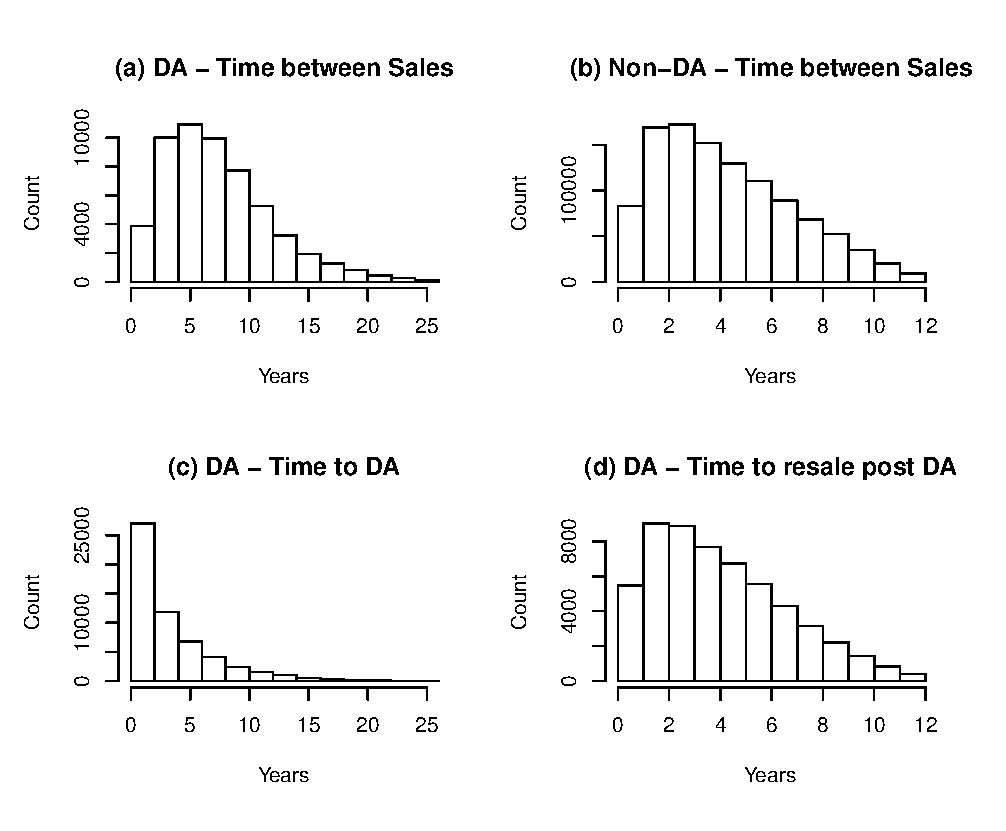
\includegraphics[width=\columnwidth]{Figures/Rplot_time_bet_sales_notional2004.eps} \par
 \caption{Distribution of Holding Term for Improved and Unimproved Homes and Time of Sale relative to DA for Improved Homes}
 \label{fig:Rplot_month_bet_sale_notional}
 \caption*{\small Figure (a) and (b) show the distribution of holding term for improved and unimproved homes respectively. Figures (c) shows the distribution of time to DA i.e. After purchasing the home, how long does one wait to carry out home improvement and figure (d) shows the distribution of time to resale post home improvement i.e how long does one stay in their home after improvement.}
  \vspace*{-\baselineskip}
 \end{figure}


We find that homeowners tend to carry out improvements as soon as they purchase their homes and therefore have longer time on average to consume the home improvement. This is also evident in figure \ref{fig:Rplot_month_bet_sale_notional}d that shows longer time to resale post improvement. Households who buy and sell within two years tend to have an investment motive \textit{a priori} and therefore can be considered as speculators on property purchase and home improvements. On the other hand, households who stay in their home for longer term but sell within two years of undertaking improvements could also be speculating on home improvements. Therefore, they cannot be assumed to have an investment motive \textit{a priori} but rather a consumption motive on property purchase and possibly a speculative motive on home improvements. Such houses can be considered as consumers for home purchase but potential speculators on home improvements.


%6.867906	3.745520
%2.900077	3.520697


%reference -- The production function for housing: evidence from france.. Combes, Duranton, Gobillon

%\clearpage

\section{Model Estimation and Results}

% There are several sources of variation in the returns. One of the major sources of variations is the market appreciation.Also the time between the sales could be significantly different for each individual property and this could affect the returns too. Therefore the variation in the returns due to time between sales is controlled for by the age of the property. Another source of variation can come from the time of purchase. To account for this, we include the years fixed effects at the time of purchase. To control for any geographical effects, we allow for location fixed effects at the State level. 

To test the returns earned by the homeowner who completes home improvement vis-à-vis the homeowner that undertakes no planning and building work post the purchase of a home, we estimate the model in equation \ref{eq:estimate} using the following general form,
\begin{equation}
    Y_i = DA_i + \beta{MktReturn_{ssd}} + \gamma_1{Age_i} + \gamma_2{Age_i^2} + Year_i + Location_i + \mu{K_i} + \epsilon_i
\end{equation}

Where, $Y_i$ is the log return of the resale price divided by notional purchase price of property $i$. The notional purchase price for unimproved homes is the purchase price on the purchase date, whereas for improved homes, the notional purchase price is the expected price at the time of DA plus the total spending on home improvement works. This total cost is referred to as the notional purchase price for improved homes since this is the equivalent cost that a homeowner will have to pay if they were to buy the house at the time of development approval and then spend on the home improvement. The expected price at the time of DA approval is calculated as the purchase price of property $i$, indexed to the point of development approval using hedonic house price indices ($HPI$) provided by CoreLogic at the Statistical Subdivision region (SSD)\footnote{The Statistical Subdivision is an Australian Standard Geographical Classification (ASGC) defined area which represents an intermediate level, general purpose, regional type geographic unit. SSDs consist of one or more Statistical Local Areas (SLAs) and cover, in aggregate, the whole of Australia without gaps or overlaps \citep{SSD}.}\footnote{In order to validate, if the SSD House Price Index are a good predictor of expected house price, we leverage the repeat sales information. We find the expected house price at the time of resale and then compare it against the actual resale price. Specifically, we calculate the percent prediction errors as $(E(P_{+1})/P_{+1}-1)*100$ and plot the distribution as shown in appendix. We find that the error distribution is normal distributed and centered around the zero mean. The empirical densities are similar to the theoretical densities.}. Specifically, the log returns for unimproved and improved homes is calculated as,

\begin{equation}
    Y_i = \left\{
    \begin{array}{l l}
      ln[P_{i,+1}/(E(P_{i,0})+ DACost_{i,0})] & \text{ Improved Homes}\\
      ln[P_{i,+1}/P_{i,-1}] & \text{ Unimproved Homes} \\
    \end{array} \right.
\end{equation}

where $E(\cdot)$ is the expectation and the expected house price at time T = 0 is given by, \begin{equation}
    E(P_{i,0}) = P_{i,-1} * (HPI_{ssd,0} / HPI_{ssd,-1})
\end{equation}

As home improvement costs are reported as of the development approval date and not at the time of completion, we calculate the expected house price at the point of development approval as it allows the expected value of the home to be expressed in the same dollar terms as at the time of development approval. For improved homes, the resale value of the property post improvement should be equal to the notional purchase price plus the additional housing value created from home improvement. Since homes with no improvements have no added housing value, comparing the returns for improved homes with unimproved homes provide us with the identification strategy for estimating returns attributable to home improvement. 

Depending on the model specification, $DA$ is a binary dummy variable coded as $1$ for improved homes and $0$ for unimproved homes or a categorical variable representing the different home improvements types. $MktReturn_{ssd}$ is the log return on the market index and captures the return attributed to the market appreciation. $Mkt$ is calculated using the SSD-specific hedonic House Price Index ($HPI$) as,

\begin{equation}
    Mkt_i = \left\{
    \begin{array}{l l}
      ln[HPI_{ssd,+1}/HPI_{ssd,0}] & \text{ Improved Homes}\\
      ln[HPI_{ssd,+1}/HPI_{ssd,-1}] & \text{ Unimproved Homes} \\
    \end{array} \right.
\end{equation}

For improved homes, $Age$ is a measure of number of months between the development completion and resale, while for unimproved homes, it is the number of months between purchase and resale. Therefore, $Age$ captures the monthly depreciation effect of the non-durable consumption, i.e. the building value. For improved homes, the time of development completion is calculated as the time when building approval is received plus the average commencement time plus the average construction time by different improvement types\footnote{\citet{abs_house_times_commence} and \citet{abs_house_times} provide the average commencement and construction times for new houses. Average construction time for swimming pool is available from \citep{hi_swimming_time}. The other values are calculated on a pro-rata basis of the average cost of home improvement}. Hence, $Age$ calculated in months is given as, 

\begin{equation}
    Age_i = \left\{
    \begin{array}{l l}
      T_{i,+1}-(T_{i,0} + C_q + C_q') & \text{ Improved Homes}\\
      T_{i,+1}-T_{i,-1}  & \text{ Unimproved Homes} \\
    \end{array} \right.
\end{equation}

where,$T_{i,+1}$ is the time of resale for property $i$, $T_{i,-1}$ is the time of purchase for property $i$, $T_{i,0}$ is the time of development approval for improved property $i$. $C_q$ and $C_q'$ represent average commencement and construction times by different improvement types q respectively. Some model specifications also include $Age_i^2$ that the captures quadratic depreciation. $Years$ is the year fixed effects at notional purchase. $Location$ is the location fixed effects at the State level\footnote{As there may be within-state variation in house prices that can affect the returns, we also test the results by controlling for the location fixed effects at SSD level. See appendix table A2}. $K_i$ is a set of control factors namely - number of beds, baths and cars.




% Table generated by Excel2LaTeX from sheet '9 june 2017'
\begin{table}[!p]
  \centering
  \caption{Variable Descriptions and Sample Summary Statistics}
  \resizebox{0.93\textwidth}{!}{

  
    \begin{tabu} to \textwidth {X[2,l]X[3,l]X[0.6,c]X[0.6,c]X[0.6,c]}
    \toprule
          &       & \multicolumn{1}{c}{Overall} & \multicolumn{1}{c}{Improved} & \multicolumn{1}{c}{Unimproved} \\
\cmidrule{3-5}    Name  & Description & \multicolumn{1}{c}{Mean} & \multicolumn{1}{c}{Mean} & \multicolumn{1}{c}{Mean} \\
   &    &   \multicolumn{1}{c}{(Std. Deviation)} & \multicolumn{1}{c}{(Std. Deviation)} & \multicolumn{1}{c}{(Std. Deviation)} \\
    \midrule
     
     Number of observations &       & \multicolumn{1}{c}{1,145,547} & \multicolumn{1}{c}{55,733} & \multicolumn{1}{c}{1,089,814} \\
    &&&&\\
    
    Purchase Price & House price at first sale & \multicolumn{1}{c}{380,867} & \multicolumn{1}{c}{436,829} & \multicolumn{1}{c}{378,005} \\
          &       & \multicolumn{1}{c}{(319,547)} & \multicolumn{1}{c}{(410,073)} & \multicolumn{1}{c}{(313,949)} \\
   Expected Purchase Price at DA  &   Purchase Price indexed to DA (DA homes)    &       & \multicolumn{1}{c}{554,532} &  \\
          &       &       & \multicolumn{1}{c}{(478,355)} &  \\
    DA cost & Cost of developments as reported in development applications &       & \multicolumn{1}{c}{104,345} &  \\
          &       &       & \multicolumn{1}{c}{(165,288)} &  \\
    Purchase price (notional) & Price at purchase for unimproved homes; Indexed Purchase Price plus cost of development for DA homes & \multicolumn{1}{c}{391,670} & \multicolumn{1}{c}{658,879} & \multicolumn{1}{c}{378,005} \\
          &       & \multicolumn{1}{c}{(333,766)} & \multicolumn{1}{c}{(536,042)} & \multicolumn{1}{c}{(313,949)} \\
    Resale Price & House price at second sale & \multicolumn{1}{c}{506,030} & \multicolumn{1}{c}{887,089} & \multicolumn{1}{c}{486,542} \\
          &       & \multicolumn{1}{c}{(411,784)} & \multicolumn{1}{c}{(723,141)} & \multicolumn{1}{c}{(379,065)} \\
    SSD specific hedonic index growth rate & Annual average growth rate of statistical sub-division specific hedonic Index for property type 'house' for period 1990 - 2016 & \multicolumn{1}{c}{0.073} &       &  \\
    Log Returns & log(Resale price / Purchase price (notional)) & \multicolumn{1}{c}{0.279} & \multicolumn{1}{c}{0.304} & \multicolumn{1}{c}{0.277} \\
          &       & \multicolumn{1}{c}{(0.409)} & \multicolumn{1}{c}{(0.422)} & \multicolumn{1}{c}{(0.408)} \\
    Months between sales (notional) & No of months between sales for non modified homes; No. of months between notional purchase and resale for DA homes  &   \multicolumn{1}{c}{50.2}   & \multicolumn{1}{c}{47.7} & \multicolumn{1}{c}{50.4} \\
    
       &       & \multicolumn{1}{c}{(31.5)} & \multicolumn{1}{c}{(30.9)} & \multicolumn{1}{c}{(31.5)}\\
    
  %  DA Types & Duplex, Extension/Alteration, Garages/Sheds \& Carports,House/Single Dwelling, Multiple DA, Swimming Pool and Verandahs \& Pergolas &       &       &  \\
    \bottomrule \\[-1.8ex]
    
     \multicolumn{5}{l}{\parbox{19cm}{\LARGE This table shows the summary statistics for the main variables, directly or indirectly, used in our model. We have a total of 1.1m records used in our model with 55,733 improved homes as our treatment sample and 1.08m unimproved homes as our control sample. The average purchase price for improved and unimproved homes is \$436,829 with a standard deviation of \$410,073 and \$378,005 with a standard deviation of \$313,949. The expected purchase price at the time of DA, for improved homes is \$554,532 and with average improvement cost of \$104,345, the average notional purchase price is \$658,879 with a standard deviation of \$536,042. The notional purchase price for unimproved homes is same as the purchase price. The average resale price for improved and unimproved homes is \$887,089 with standard deviation of \$723,141 and \$486,542 with standard deviation of \$379,065 respectively. The large standard deviation of improved homes is mainly due to the different types of home improvements as some improvements for e.g. verandas/pergolas add little value while others e.g. Duplex adds more value to the homes. The average annual growth rate of Statistical Subdivision level Hedonic House Price Index used to calculate the expected purchase price and also the market return is 7.3\%. We see that the average log return of the resale price to the notional purchase price (i.e. after accounting for the cost of improvement) for improved homes is 30.4\% with a standard deviation of 42.2\%. While for unimproved homes the average log return is 27.7\% with a standard deviation of 40.8\%. In terms of univariate results, this may suggest that the return for improved homes is, on average, 2.7\% higher than unimproved homes. However, the univariate results do not control for factors such as time of purchase and resale, depreciation of the home, and property attributes such as number of beds, baths and cars which is possible in the regression model. After controlling for these factors in the regression, we find that the returns for improved homes are in fact lower, on average, than unimproved homes by 2.4\%. The average time between sales for unimproved homes is 47.7 months while for improved homes the average time between DA and resale (i.e. the time between notional purchase and resale) is 50.4 months. These are the times for which the households have consumed the housing service and allows for capturing the depreciation effect of the property.}}
    
    % the figures reported in unimproved home are for 1.08m are post 2004, but the need to be checked for constant dollars of 2016..and then update the figures above in notes..
    
    \end{tabu} %
        }
 
  \label{tab:variable_statistics}%
  
\end{table}%


Table \ref{tab:variable_statistics} shows the summary statistics for the main variables used in our model. We have a total of 1.1m records used in our model with 55,733 improved homes as our treatment sample and 1.08m unimproved homes as our control sample. The average purchase price for improved and unimproved homes is \$436,829 with a standard deviation of \$410,073 and \$378,005 with a standard deviation of \$313,949. The expected purchase price at the time of DA, for improved homes is \$554,532 and with average improvement cost of \$104,345, the average notional purchase price is \$658,879 with a standard deviation of \$536,042. The notional purchase price for unimproved homes is same as the purchase price. The average resale price for improved and unimproved homes is \$887,089 with standard deviation of \$723,141 and \$486,542 with standard deviation of \$379,065 respectively. The large standard deviation of improved homes is mainly due to the different types of home improvements as some improvements for e.g. verandas/pergolas add little value while others e.g. Duplex adds more value to the homes.

The average annual growth rate of Hedonic House Price Index (at Statistical Subdivision level) used to calculate the expected purchase price and also the market return is 7.3\%. We see that the average log return of the resale price to the notional purchase price (i.e. after accounting for the cost of improvement) for improved homes is 30.4\% with a standard deviation of 42.2\%. While for unimproved homes the average log return is 27.7\% with a standard deviation of 40.8\%. In terms of univariate results, this may suggest that the return for improved homes is, on average, 2.7\% higher than unimproved homes. However, the univariate results do not control for factors such as time of purchase and resale, depreciation, and property attributes -- number of beds, baths and car spaces, which is possible in a regression model. After controlling for these factors in the regression, we find that the returns for improved homes are in fact lower, on average, than unimproved homes by 2.4\%. The average time between sales for unimproved homes is 47.7 months while for improved homes the average time between DA and resale (i.e. the time between notional purchase and resale) is 50.4 months. These are the times for which the households have consumed the housing service and allows for capturing the depreciation effect of the property.




As the development is completed, in addition to the building value - $B_0'$, there is unobserved housing value - $H'$ produced which is the value of the home improvement. While the cost is explicitly observed at the time of development approval, the home improvement value is unobserved but is implicitly observed only in the resale price. This provides for our identification strategy. Now, since the value $H'$ is only identified between the time of development approval and resale, returns from the time of purchase to the point of development approval can only be attributed to the market appreciation and therefore any variation in the returns prior to the point of development approval does not contribute to the identification of home improvement value. Hence, to implement our identification strategy, we use the notional purchase price in calculating the returns for improved homes. Moreover, using the notional purchase price, puts the purchase price and the improvement cost in the same dollar terms as at time of improvement of the property, thereby allowing us to directly add the expected price at the time of development approval and improvement cost (also reported at the time of development approval) to arrive at the notional purchase price. Also, since, we do not have to move the cost of spending across time, this strategy is free from relying on any assumption of using an appropriate cost-of-funds rate. 

Also, according to \citet{rosenthal1999residential} the implicit market for residential buildings is efficient and the inefficiencies in the housing market must lie in the market for land itself and therefore the prices of houses (including the building component in the house price index) should adjust themselves fast enough so as to eliminate any excess profit opportunities for builders. Hence, since, the building component in the house price index is efficient and the land between the time of purchase and resale remains fixed and does not change with home improvement, our model should be free from any market inefficiency bias.

The identification of the home improvement value comes from controlling for the common sources of variation in the improved and unimproved house prices that affect the returns. A major source of variation in the house price return is attributed to the market appreciation which is captured using the return on the house price index. Another source of variation is the time between notional purchase and resale. Since, for improved homes, this is also the time between home improvement and resale. This variable captures the depreciation effect due to aging of the existing and the additional building value created from home improvement. Another potential source of variation in the returns is the area of the land. Due to the limited information on land area, we use number of beds, baths and cars to proxy for the land area. As our model calculates returns on notional purchase price, any variations in returns between purchase and point of DA are already captured in the expected price using the SSD index. Once the common sources of variations between improved and unimproved homes are controlled for, the difference in the returns would then only be attributable to the home improvement. Hence in order to identify that variation, we simply use a binary dummy variable to capture the differences in the returns between improved and unimproved homes.

Table \ref{tab:results} shows the estimation results for different model specifications\footnote{Since the returns are modelled in log form, the coefficients are interpreted as ($e^{\hat{\beta}}-1$) for small values of $\beta$. Robust standard errors are reported in parenthesis and the significance of the variables is adjusted according to the robust standard errors.}. All models allow for year and state\footnote{Model results with location fixed effects at SSD level are provided in appendix table A2. The results are consistent with the main results across all model specifications. At aggregate level, the returns for improved homes are 1.9\% and 2.4\% lower than unimproved homes respectively. We also note that after controlling for location fixed effects at the SSD level, the $MktReturn$ variable captures around 95\% of the variations in the return as compared to 92\% with State fixed effects.} fixed effects. Model 1 is the basic model with house price log returns regressed only on the market index and no controls. The coefficient on the Mkt is 0.749 which indicates that 75\% of the appreciation in the house prices is due to the market. Model 2 includes the property attributes at the time of resale and model 3 includes the property attributes for both, at the time of resale and purchase. The coefficients on both, purchase and resale attributes are significant, with values for number of beds, baths and cars at resale as 2.6\%, 5.8\% and 0.4\% and -3.2\%, -6.2\% and -1.5\% at time of purchase respectively. This indicates that, other factors constant, the return is higher if one buys a smaller house and sells a bigger house and vice-versa. In model 3, we see that the variation captured by the market returns has improved to 80\%. 

In model 4, we include age as a linear term while in model 5 we include age as a quadratic term. The age captures the depreciation effect of the property attributed to the non-durable consumption. The coefficient on age in the linear form indicates that the returns on the property decreases by 0.1\% every month due to the depreciation. In the quadratic form, the coefficient on age is -0.2\% while the coefficient on squared age is positive. Since the age is measured in months, the coefficient on the quadratic term (the curvature) is quite small but statistically significant and therefore we include the squared term in the full model. The coefficients in the attributes at the time of purchase and resale are consistent with the previous models. Also the variation in the returns captured by the market appreciation further improves to 92\%. 

Models 1 to 5, present returns for each of the home improvement types, relative to unimproved homes. Models 5 is a full model with control for market appreciation and other attributes. Depending on the model specification, the returns on each of improvement types are not attributed to the market appreciation and other attributes as they are already controlled for explicitly. Also any omitted or unobserved (deterministic) factors will be captured in the constant. Hence the returns on each of the improvement types are over and above the returns for unimproved homes. 

\newgeometry{margin=0.5in}
% Table created by stargazer v.5.2 by Marek Hlavac, Harvard University. E-mail: hlavac at fas.harvard.edu
% Date and time: Fri, Jun 30, 2017 - 10:00:05 AM
% Requires LaTeX packages: dcolumn rotating 


\begin{sidewaystable}[!htbp] \centering 
  \caption{Main Model Results} 
  \label{tab:results} 
  \resizebox{\textwidth}{!}{
  \begin{threeparttable}

\begin{tabular}{@{\extracolsep{5pt}}lD{.}{.}{-3} D{.}{.}{-3} D{.}{.}{-3} D{.}{.}{-3} D{.}{.}{-3} D{.}{.}{-3} } 
\\[-1.8ex] 
\toprule \\[-1.8ex] 
\\[-1.8ex] & \multicolumn{6}{c}{Log(Resale Price/Purchase Price (Notional))} \\ 
\\[-1.8ex] & \multicolumn{1}{c}{(1)} & \multicolumn{1}{c}{(2)} & \multicolumn{1}{c}{(3)} & \multicolumn{1}{c}{(4)} & \multicolumn{1}{c}{(5)} & \multicolumn{1}{c}{(6)}\\ 
\midrule \\[-1.8ex] 
 DA &  &  &  &  & -0.019^{***} & -0.024^{***} \\ 
  &  &  &  &  & (0.002) & (0.002) \\ 
  %& & & & & & \\ 
 Carports/Garages/Sheds & -0.022^{***} & -0.021^{***} & -0.021^{***} & -0.025^{***} &  &  \\ 
  & (0.007) & (0.007) & (0.007) & (0.007) &  &  \\ 
  %& & & & & & \\ 
 Duplex & 0.094^{***} & 0.097^{***} & 0.098^{***} & 0.101^{***} &  &  \\ 
  & (0.013) & (0.013) & (0.013) & (0.013) &  &  \\ 
  %& & & & & & \\ 
 Extension/Alteration & 0.001 & 0.001 & 0.000 & -0.001 &  &  \\ 
  & (0.004) & (0.004) & (0.004) & (0.004) &  &  \\ 
  %& & & & & & \\ 
 House/Single Dwelling & -0.105^{***} & -0.101^{***} & -0.100^{***} & -0.102^{***} &  &  \\ 
  & (0.007) & (0.007) & (0.007) & (0.007) &  &  \\ 
  %& & & & & & \\ 
 Multiple DA & -0.018^{***} & -0.012^{*} & -0.011^{*} & -0.017^{***} &  &  \\ 
  & (0.006) & (0.006) & (0.006) & (0.006) &  &  \\ 
  %& & & & & & \\ 
 Swimming Pool & -0.001 & 0.004 & 0.004 & -0.005 &  &  \\ 
  & (0.003) & (0.003) & (0.003) & (0.003) &  &  \\ 
  %& & & & & & \\ 
 Verandahs/Pergolas & -0.039^{***} & -0.037^{***} & -0.038^{***} & -0.042^{***} &  &  \\ 
  & (0.004) & (0.004) & (0.004) & (0.004) &  &  \\ 
  %& & & & & & \\ 
 MktReturn & 0.804^{***} & 0.923^{***} & 0.922^{***} & 0.924^{***} & 0.923^{***} & 0.925^{***} \\ 
  & (0.003) & (0.003) & (0.003) & (0.003) & (0.003) & (0.003) \\ 
  %& & & & & & \\ 
 Months between sales &  & -0.001^{***} & -0.002^{***} & -0.002^{***} & -0.002^{***} & -0.002^{***} \\ 
  &  & (0.000) & (0.000) & (0.000) & (0.000) & (0.000) \\ 
  %& & & & & & \\ 
 Months between sales squared &  &  & 0.000^{***} & 0.000^{***} & 0.000^{***} & 0.000^{***} \\ 
  &  &  & (0.000) & (0.000) & (0.000) & (0.000) \\ 
  %& & & & & & \\ 
 No. of beds (resale) & 0.026^{***} & 0.027^{***} & 0.026^{***} &  & 0.026^{***} &  \\ 
  & (0.001) & (0.001) & (0.001) &  & (0.001) &  \\ 
  %& & & & & & \\ 
 No. of baths (resale) & 0.058^{***} & 0.059^{***} & 0.059^{***} &  & 0.059^{***} &  \\ 
  & (0.001) & (0.001) & (0.001) &  & (0.001) &  \\ 
  %& & & & & & \\ 
 No. of cars (resale) & 0.004^{***} & 0.006^{***} & 0.006^{***} &  & 0.006^{***} &  \\ 
  & (0.000) & (0.000) & (0.000) &  & (0.000) &  \\ 
  %& & & & & & \\ 
 No. of beds (purchase) & -0.032^{***} & -0.033^{***} & -0.033^{***} &  & -0.032^{***} &  \\ 
  & (0.001) & (0.001) & (0.001) &  & (0.001) &  \\ 
  %& & & & & & \\ 
 No. of baths (purchase) & -0.069^{***} & -0.069^{***} & -0.069^{***} &  & -0.068^{***} &  \\ 
  & (0.001) & (0.001) & (0.001) &  & (0.001) &  \\ 
  %& & & & & & \\ 
 No. of cars (purchase) & -0.015^{***} & -0.016^{***} & -0.016^{***} &  & -0.016^{***} &  \\ 
  & (0.000) & (0.000) & (0.000) &  & (0.000) &  \\ 
  %& & & & & & \\ 
 Change in \# of beds &  &  &  & 0.029^{***} &  & 0.029^{***} \\ 
  &  &  &  & (0.001) &  & (0.001) \\ 
  %& & & & & & \\ 
 Change in \# of baths &  &  &  & 0.063^{***} &  & 0.062^{***} \\ 
  &  &  &  & (0.001) &  & (0.001) \\ 
  %& & & & & & \\ 
 Change in \# of cars &  &  &  & 0.010^{***} &  & 0.010^{***} \\ 
  &  &  &  & (0.000) &  & (0.000) \\ 
  %& & & & & & \\ 
 Constant & 0.088^{***} & 0.114^{***} & 0.129^{***} & 0.078^{***} & 0.129^{***} & 0.078^{***} \\ 
  & (0.002) & (0.002) & (0.003) & (0.002) & (0.003) & (0.002) \\ 
  %& & & & & & \\ 
Year Fixed Effects & Yes & Yes & Yes & Yes & Yes &  \\ 
Location Fixed Effects & Yes & Yes & Yes & Yes & Yes &  \\ 
Observations & \multicolumn{1}{c}{517,011} & \multicolumn{1}{c}{517,011} & \multicolumn{1}{c}{517,011} & \multicolumn{1}{c}{517,011} & \multicolumn{1}{c}{517,011} & \multicolumn{1}{c}{517,011} \\ 
Adjusted R$^{2}$ & \multicolumn{1}{c}{0.281} & \multicolumn{1}{c}{0.289} & \multicolumn{1}{c}{0.290} & \multicolumn{1}{c}{0.287} & \multicolumn{1}{c}{0.289} & \multicolumn{1}{c}{0.287} \\ 
F Statistic & \multicolumn{1}{c}{6,528.365$^{***}$ (df = 31; 516979)} & \multicolumn{1}{c}{6,580.655$^{***}$ (df = 32; 516978)} & \multicolumn{1}{c}{6,398.490$^{***}$ (df = 33; 516977)} & \multicolumn{1}{c}{6,954.690$^{***}$ (df = 30; 516980)} & \multicolumn{1}{c}{7,793.277$^{***}$ (df = 27; 516983)} & \multicolumn{1}{c}{8,663.804$^{***}$ (df = 24; 516986)} \\ 


%F Statistic & \multicolumn{1}{H}{6,097.764$^{***}$ (df = 27; 1145334)} & \multicolumn{1}{H}{6,085.191$^{***}$ (df = 30; 1035385)} & \multicolumn{1}{H}{6,111.101$^{***}$ (df = 33; 525110)} & \multicolumn{1}{H}{6,167.475$^{***}$ (df = 34; 525109)} & \multicolumn{1}{c}{6,007.371$^{***}$ (df = 35; 525108)} & \multicolumn{1}{c}{6,493.052$^{***}$ (df = 32; 525111)} & \multicolumn{1}{c}{7,225.539$^{***}$ (df = 29; 525114)} & \multicolumn{1}{c}{7,964.678$^{***}$ (df = 26; 525117)} \\ 

\bottomrule \\[-1.8ex] 
%\multicolumn{9}{p{1.2\textwidth}}{Robust standard errors are reported in parentheses, Significance of variables is adjusted accordingly. *** 0.1\% significance ** 1\% significance * 5\% significance. We have a total of 1,145,547 (55,733 for treatment and 1,089,814 for control sample) possible observation with deviation accounted for by missing data.} \\ 
\end{tabular}

 \begin{tablenotes}[para,flushleft]
  \LARGE
      Notes: Robust standard errors are reported in parentheses, Significance of variables is adjusted accordingly. *** 0.1\% significance ** 1\% significance * 5\% significance. We have a total of 1,119,419 (55,733 for treatment and 1,063,686 for control sample) possible observation with deviation accounted for by missing data.
\end{tablenotes}    

    \end{threeparttable}


}
\end{sidewaystable} 
\restoregeometry

The results show that the returns for carports are negative and mostly insignificant across models specifications. The coefficient on duplexes, in the full model, suggests that the return for a duplex is 9.8\% higher than the unimproved homes. Also, across all models, the results for duplexes are consistently positive and significant ranging between 8.4\% to 18\%. For Extension/Alterations, the returns are insignificant across models with controls. In case of House/Single Dwelling, the returns are consistently negative and strongly significant in all model specifications. The full model coefficient on House/Single Dwelling is -0.10 indicating that the returns for House/Single Dwelling is around 10\% lower than unimproved homes. For Multiple DAs, on average, the results are mostly negative and significant across models. In the full model, the return on Multiple DAs is 1.1\% lower than the unimproved homes. In case of Swimming pools, when there is no control for attributes at the time of purchase, the returns are almost 18\% and 14\% higher than unimproved homes. However when we control for the purchase attributes, the returns become insignificant. And when we include depreciation, the returns are marginally positive and significant at 0.4\%. For verandas/pergolas, the returns are mostly negative and strongly significant. In the full model, the return on verandas and pergolas is 3.8\% lower than unimproved homes.

The model 1 does not have any control attributes and therefore it assumes that all properties are bought and sold are of the same size. Model 2 controls for the attributes at the time of resale and therefore assumes that all homes bought are of the same size. And in model 3, we control for the size at both, the time of purchase and resale. However, although we account for the size of the house using number of beds, baths and cars, the size in terms of land area could still vary significantly and therefore have some unidentified variations in returns. 

When the homeowner carries out developments, the attributes post improvement or at resale are likely to be higher than at the time of purchase, or remain unchanged if the homeowner does no development. Therefore the attributes at resale are quite likely to be correlated with attributes at purchase. In models 3, 4 and 5, we have both, attributes at the time of resale and purchase included as independent variables that may lead to problem of multi-collinearity. Hence, in order to resolve the problem of multi-collinearity, we also run the model with an alternate specification - model 6, where we include change in the corresponding attributes as an independent variable. A disadvantage of taking change in attributes could be that we lose information on the absolute level of the attributes which provides a proxy for the land area. Implicitly, this model assumes that returns for a homeowner who buys a 1 bedroom and sells a two bedroom will be the same as for someone who buys a two bedroom and sells a three bedroom house as the change in no. of bedrooms is the same in both cases. Considering the merits of both model specifications, we present and examine the results on both model specifications - 5 and 6 for different improvement types and 7 and 8 for aggregate level, in this paper.

The finding in the alternate model specification are also consistent with overall results. The returns on carports/garages/sheds and verandas/pergolas is 2.5\% and 4.2\% lower than the unimproved homes respectively. For Duplex the returns are 10.1\% higher than unimproved homes. For extension/alteration and swimming pools, the returns are not significantly different from unimproved homes. In case of House/Single Dwelling, the return are strongly negative by 10.2\% as compared to unimproved homes. Finally, for multiple DAs, the average returns are 4.2\% below unimproved homes. The coefficient on the $Mkt$ is 92.2\% same as the model 5. The change in no. of beds, baths and cars are all positive indicating that greater the difference between size of the house before and after improvement, higher are the returns. 

Overall, across different home improvement types, we find that the returns for carports/garages/sheds, multiple DAs and verandas/pergolas are negative relative to the unimproved homes while for house/single dwelling, the return is strongly negative. The returns for extension/alterations and swimming pools is not significantly different from unimproved homes. In contrast, the return for duplexes is strongly positive.

One of the reasons that explains why the returns on house/single dwelling, is strongly negative is due to the opportunity cost. In building a new house, unlike extension/alteration where the homeowner produces additional housing by building on top of the existing building, the homeowner demolishes the existing building and therefore loses the entire residual value of the building $B_0$ (i.e. the non-durable consumption value) plus the value of housing service $H_0$ (i.e. the durable consumption) in the process. The homeowner then builds the house from the scratch and therefore has to pay for the whole building value again.

According to \citet{potepan1989interest}, carrying out developments on existing house have technological constraints. For example, the presence of existing housing constraints the home improvement by impeding the application of certain construction techniques common in new housing production. For relatively modest increases in housing units, this technological difference is probably negligible, but for sizable increases, this technological constraint results in higher average costs in home improvement. Therefore in building a new house there are efficiency gains as compared to extension/alterations. Hence, for new houses, the some of the loss from the opportunity costs are reduced by the extent of the efficiency gains availed from the lack of impediment.

Like building a new house, duplex also has high opportunity cost as it also requires to demolish the old property and therefore lose all residual value of the existing building. But the returns on duplexes are much higher than the unimproved homes? This because of the land split. All the properties that are converted into a duplex as part of improvement, are purchased as a single block of land, originally allocated for single-family dwelling. When applying for development application for duplexes, homeowners can split the block of land and convert it to a dual occupancy use\footnote{For example, if the original property is on 1/13 Cragg street, then after the split the two duplexes will be addressed - 1/13 and 1A/13 Cragg Street.}. Now homeowners are able to build two identical duplexes for two single families. The homeowners can sell one duplex and reside in the other or sell both\footnote{If the homeowner sells only one duplex then we only have one observed record and if they sell both, then to avoid duplication, we just take one record and double the resale price.}.  Either way, the homeowners have created twice as much equity from selling two duplexes. However the resale price observed in the data set corresponds only to one duplex\footnote{This is because if the other duplex is not sold, valued or financed, then that duplex is not recorded in CoreLogic's database.}. Therefore for duplexes, we double the resale price to adjust for the double equity. Hence, the return on Duplexes are strongly positive although partly offset by the losses due to lost residual value.

When homeowners carry out alteration/extension, the fundamental cost of the improvement they should pay for is the cost of building materials plus the labour cost. With the completion of development, there is an additional value of housing service produced for the homeowners which is unobserved at that time but observed implicitly at the time of resale. Some portion of this expected value created from home improvement is priced into the cost of development. This could also be the contribution factor for why the returns for alteration/extension is insignificant.
Apart from this there is some portion of the building value that is depreciated away and therefore we find, insignificant profits after controlling for market appreciation. In case of swimming pool, in addition to the reasons discussed for extension/alterations, the insignificant returns can be attributed to the perceived cost of operating the swimming pool on a regular basis and therefore, depending on the preferences, prospective buyers may not value the utility of the swimming pool and therefore the homeowner may not get a better resale price.

Models 7 and 8 are the aggregate level results corresponding to model specifications 5 and 6 respectively. The coefficient on DA dummy represents the returns for improved homes relative to unimproved homes. Based on models 7 and 8, we find that, the returns for the improved homes are, in expectation, 1.9\% and 2.4\% lower than the unimproved homes respectively. Therefore homeowners who do nothing are relatively better off than those who improve their homes. 

\clearpage

\section{Further Analysis}

In the previous section, we compared the returns for all improved homes with unimproved homes and found that the returns for improved homes is lower than unimproved homes. In this section, we perform further analysis to examine how the returns for homeowners with a speculative motive perform for improved homes with respect to the unimproved homes. People who buy and sell the property in short term are more likely to have a speculative motive at the onset and therefore we identify homeowners that buy and sell the property within two years as speculators and those who buy and sell in more than two years as non-speculators\footnote{We take two years as a reasonable approximation of the upper limit of the time between sales required to identify home buyers with the intention of buying the property with an speculative motive. Any longer period between sales decreases the likelihood that homeowner bought the property with the intent of pure speculation.}.

% Table created by stargazer v.5.2 by Marek Hlavac, Harvard University. E-mail: hlavac at fas.harvard.edu
% Date and time: Wed, Jun 21, 2017 - 11:23:41 AM
% Requires LaTeX packages: dcolumn rotating 
\begin{table}[!p] \centering 
  \caption{Results for Speculator Type I and Non-Speculator Groups} 
  \label{tab:results_s0_investor_da_interaction} 
  \resizebox{0.7\textwidth}{!}{
\begin{tabular}{@{\extracolsep{5pt}}lD{.}{.}{-3} D{.}{.}{-3} } 
\\[-1.8ex] 
\toprule \\[-1.8ex] 
\\[-1.8ex] & \multicolumn{2}{c}{Log(Resale Price/Purchase Price (Notional))} \\ 
\\[-1.8ex] & \multicolumn{1}{c}{(1)} & \multicolumn{1}{c}{(2)}\\ 
\midrule \\[-1.8ex] 
 DA & -0.021^{***} & -0.025^{***} \\ 
  & (0.002) & (0.002) \\ 
  & & \\ 
 Investor & 0.007^{***} & 0.007^{***} \\ 
  & (0.001) & (0.001) \\ 
  & & \\ 
  DA:Investor & 0.025^{***} & 0.026^{***} \\ 
  & (0.006) & (0.006) \\ 
  & & \\ 
 MktReturn & 0.921^{***} & 0.923^{***} \\ 
  & (0.003) & (0.003) \\ 
  & & \\ 
 Age & -0.002^{***} & -0.002^{***} \\ 
  & (0.000) & (0.000) \\ 
  & & \\ 
 Age Square & 0.000^{***} & 0.000^{***} \\ 
  & (0.000) & (0.000) \\ 
  & & \\ 
 No. of beds (Resale) & 0.026^{***} &  \\ 
  & (0.001) &  \\ 
  & & \\ 
 No. of baths (Resale) & 0.058^{***} &  \\ 
  & (0.001) &  \\ 
  & & \\ 
 No. of cars (Resale) & 0.006^{***} &  \\ 
  & (0.000) &  \\ 
  & & \\ 
 No. of beds (Purchase) & -0.033^{***} &  \\ 
  & (0.001) &  \\ 
  & & \\ 
 No. of baths (Purchase) & -0.067^{***} &  \\ 
  & (0.001) &  \\ 
  & & \\ 
 No. of cars (Purchase) & -0.016^{***} &  \\ 
  & (0.000) &  \\ 
  & & \\ 
 Change in \# of beds &  & 0.029^{***} \\ 
  &  & (0.001) \\ 
  & & \\ 
 Change in \# of baths &  & 0.062^{***} \\ 
  &  & (0.001) \\ 
  & & \\ 
 Change in \# of cars &  & 0.010^{***} \\ 
  &  & (0.000) \\ 
  & & \\ 
 Constant & 0.126^{***} & 0.075^{***} \\ 
  & (0.005) & (0.004) \\ 
  & & \\ 
Year Fixed Effects & Yes & Yes \\ 
Location Fixed Effects & Yes & Yes \\ 
Observations & \multicolumn{1}{c}{525,144} & \multicolumn{1}{c}{525,144} \\ 
Adjusted R$^{2}$ & \multicolumn{1}{c}{0.285} & \multicolumn{1}{c}{0.283} \\ 
F Statistic & \multicolumn{1}{c}{6,761.652$^{***}$} & \multicolumn{1}{c}{7,398.417$^{***}$ } \\ 
 & \multicolumn{1}{c}{(df = 31; 525112)} & \multicolumn{1}{c}{(df = 28; 525115)} \\ 
\bottomrule \\[-1.8ex] 
\multicolumn{3}{l}{Notes: *** 0.1\% significance ** 1\% significance * 5\% significance}\\
\multicolumn{3}{l}{Robust standard errors in parentheses.} \\
\end{tabular}
}
\end{table}

For the homeowner with improved homes, we classify speculators into two types. Speculators type I (a.k.a. Flippers) are those who have a speculative motive right at the onset and therefore buy the property, improve and sell within two years of purchase\footnote{homeowner who buy with an investment motive of renting the property and sell in more than two years from buying are treated as non-speculators since this can be thought of as equivalent to someone else consuming the property on owner's behalf.}. Speculators type II are those homeowners who buy the property not with a view to sell the property in near term but to live and consume the housing and at some point later improve the property and sell it within two years of improvement. These speculators are those who improve and sell in less than two years\footnote{The time of two years is calculated from the date of DA approval and not the completion of home improvement as this time closely represents the time of their decision to improve and most probably their intent to sell post improvement.} from the time of improvement. 

\subsection{Speculators Type I / Flippers (Buy-Improve-Sell)}

Table \ref{tab:results_s0_investor_da_interaction} shows the results of the model for speculators type I / (Flippers) and non-speculator groups. DA is the dummy variable equal to 1 for improved homes and 0 for unimproved homes. Investor is also a dummy variable indicating a speculator and equals 1 if time between actual purchase and resale is less than 2 years and 0 otherwise. DA*Investor is the interaction term. Models 1 and 2 are the full model specifications at aggregate level with interaction terms. The coefficient on other model variables are all consistent with the main model results.

In models 1 and 2, for homeowners who are non-speculators, we find that results confirm our main findings. The returns for improved homes is 2.1\% and 2.5\% lower than unimproved homes respectively. However, for the speculator/flipper group, we find that the returns for improved homes, on aggregate, are significant and higher than unimproved homes by 0.4\% (-0.021 + 0.025) and 0.1\% (-0.025 + 0.026) respectively.

If we compare across speculator and non-speculator group, for unimproved homes, the return for speculator group is 0.7\% higher than the non-speculator group in both model specifications 1 and 2. If we look at improved homes, then the returns for speculator is 3.2\% (0.007 + 0.025) and 3.3\% (0.007 + 0.026) higher than non-speculators respectively.

The homeowner who do not improve their home and buy and sell within 2 years have higher returns than those who buy and sell in more than 2 years. Therefore the gap between returns of speculator and non-speculator group is much higher for improved homes than unimproved homes. This suggests that, in contrast to the main results, homeowners who have investment motive and improve their homes are better off than homeowners with investment motive but do not improve their home.

In table \ref{tab:results_s0_investor_da_type}, we split the results by improvement types and focus on speculator group only. In models 1 to 6, we present findings that correspond to the model specifications 1 to 6 in the main results. The results show that return for carports/garages/sheds has improved from significantly negative in the main results to being not significantly different from unimproved homes. The returns for Duplex is mostly around 8\% higher which is similar to the main results where the duplex return is around 10\% higher than unimproved homes. 

\newgeometry{margin=1in}
% Table created by stargazer v.5.2 by Marek Hlavac, Harvard University. E-mail: hlavac at fas.harvard.edu
% Date and time: Wed, Jun 21, 2017 - 10:58:59 AM
% Requires LaTeX packages: dcolumn rotating 
\begin{table}[!p] \centering 
  \caption{Results for Speculator I by DA works} 
  \label{tab:results_s0_investor_da_type} 
  \resizebox{\textwidth}{!}{
\begin{tabular}{@{\extracolsep{5pt}}lHH D{.}{.}{-3} D{.}{.}{-3} D{.}{.}{-3} D{.}{.}{-3} } 
\\[-1.8ex] 
\toprule \\[-1.8ex] 
\\[-1.8ex] & \multicolumn{6}{c}{Log(Resale Price/Purchase Price (Notional))} \\ 
\\[-1.8ex] & \multicolumn{1}{H}{(1)} & \multicolumn{1}{H}{(2)} & \multicolumn{1}{c}{(1)} & \multicolumn{1}{c}{(2)} & \multicolumn{1}{c}{(3)} & \multicolumn{1}{c}{(4)}\\ 
\midrule \\[-1.8ex] 

 Carports/Garages/Sheds & -0.063^{***} & -0.049^{**} & 0.018 & 0.012 & 0.013 & 0.009 \\ 
  & (0.023) & (0.024) & (0.024) & (0.024) & (0.024) & (0.024) \\ 
  %& & & & & & \\ 
 Duplex & 0.139^{***} & 0.087^{***} & 0.066^{***} & 0.087^{***} & 0.080^{***} & 0.082^{***} \\ 
  & (0.014) & (0.014) & (0.017) & (0.017) & (0.017) & (0.017) \\ 
  %& & & & & & \\ 
 Extension/Alteration & 0.082^{***} & 0.048^{***} & 0.058^{***} & 0.053^{***} & 0.055^{***} & 0.054^{***} \\ 
  & (0.008) & (0.009) & (0.010) & (0.010) & (0.010) & (0.010) \\ 
  %& & & & & & \\ 
 House/Single Dwelling & -0.111^{***} & -0.158^{***} & -0.121^{***} & -0.108^{***} & -0.110^{***} & -0.113^{***} \\ 
  & (0.012) & (0.011) & (0.017) & (0.017) & (0.017) & (0.017) \\ 
  %& & & & & & \\ 
 Multiple\_DA & 0.021 & -0.028^{*} & 0.016 & 0.024 & 0.024 & 0.019 \\ 
  & (0.015) & (0.015) & (0.020) & (0.021) & (0.021) & (0.020) \\ 
  %& & & & & & \\ 
 Swimming Pool & 0.041^{***} & 0.020 & 0.011 & 0.012 & 0.013 & 0.005 \\ 
  & (0.014) & (0.014) & (0.009) & (0.009) & (0.009) & (0.009) \\ 
  %& & & & & & \\ 
 Verandahs/Pergolas & -0.049^{***} & -0.042^{***} & 0.005 & -0.003 & -0.003 & -0.006 \\ 
  & (0.012) & (0.013) & (0.012) & (0.012) & (0.012) & (0.012) \\ 
  %& & & & & & \\ 
 MktReturn & 0.796^{***} & 0.829^{***} & 0.868^{***} & 0.931^{***} & 0.933^{***} & 0.938^{***} \\ 
  & (0.009) & (0.009) & (0.009) & (0.010) & (0.010) & (0.010) \\ 
  %& & & & & & \\ 
 Age &  &  &  & -0.003^{***} & -0.006^{***} & -0.006^{***} \\ 
  &  &  &  & (0.000) & (0.001) & (0.001) \\ 
  %& & & & & & \\ 
 Age Square &  &  &  &  & 0.000^{***} & 0.000^{***} \\ 
  &  &  &  &  & (0.000) & (0.000) \\ 
  %& & & & & & \\ 
 No. of beds (Resale) &  & 0.020^{***} & 0.031^{***} & 0.031^{***} & 0.031^{***} &  \\ 
  &  & (0.001) & (0.002) & (0.002) & (0.002) &  \\ 
  %& & & & & & \\ 
 No. of baths (Resale) &  & 0.050^{***} & 0.058^{***} & 0.059^{***} & 0.059^{***} &  \\ 
  &  & (0.002) & (0.002) & (0.002) & (0.002) &  \\ 
  %& & & & & & \\ 
 No. of cars (Resale) &  & -0.010^{***} & 0.004^{***} & 0.004^{***} & 0.004^{***} &  \\ 
  &  & (0.001) & (0.001) & (0.001) & (0.001) &  \\ 
  %& & & & & & \\ 
 No. of beds (Purchase) &  &  & -0.035^{***} & -0.035^{***} & -0.035^{***} &  \\ 
  &  &  & (0.002) & (0.002) & (0.002) &  \\ 
  %& & & & & & \\ 
 No. of baths (Purchase) &  &  & -0.067^{***} & -0.068^{***} & -0.068^{***} &  \\ 
  &  &  & (0.002) & (0.002) & (0.002) &  \\ 
  %& & & & & & \\ 
 No. of cars (Purchase) &  &  & -0.015^{***} & -0.015^{***} & -0.015^{***} &  \\ 
  &  &  & (0.001) & (0.001) & (0.001) &  \\ 
  %& & & & & & \\ 
 Change in \# of beds &  &  &  &  &  & 0.033^{***} \\ 
  &  &  &  &  &  & (0.002) \\ 
  %& & & & & & \\ 
 Change in \# of baths &  &  &  &  &  & 0.062^{***} \\ 
  &  &  &  &  &  & (0.002) \\ 
  %& & & & & & \\ 
 Change in \# of cars &  &  &  &  &  & 0.009^{***} \\ 
  &  &  &  &  &  & (0.001) \\ 
  %& & & & & & \\ 
 Constant & 0.059^{***} & -0.083^{***} & 0.054^{***} & 0.088^{***} & 0.105^{***} & 0.061^{***} \\ 
  & (0.007) & (0.008) & (0.010) & (0.010) & (0.011) & (0.011) \\ 
  %& & & & & & \\ 
Year Fixed Effects & Yes & Yes & Yes & Yes & Yes & Yes \\ 
Location Fixed Effects & Yes & Yes & Yes & Yes & Yes & Yes \\ 

Observations & \multicolumn{1}{H}{271,575} & \multicolumn{1}{H}{234,902} & \multicolumn{1}{c}{119,448} & \multicolumn{1}{c}{119,448} & \multicolumn{1}{c}{119,448} & \multicolumn{1}{c}{119,448} \\ 

Adjusted R$^{2}$ & \multicolumn{1}{H}{0.046} & \multicolumn{1}{H}{0.062} & \multicolumn{1}{c}{0.120} & \multicolumn{1}{c}{0.123} & \multicolumn{1}{c}{0.123} & \multicolumn{1}{c}{0.121} \\ 

F Statistic & \multicolumn{1}{H}{488.390$^{***}$ (df = 27; 271547)} & \multicolumn{1}{H}{518.701$^{***}$} & \multicolumn{1}{c}{495.690$^{***}$} & \multicolumn{1}{c}{492.394$^{***}$} & \multicolumn{1}{c}{479.292$^{***}$} & \multicolumn{1}{c}{513.604$^{***}$} \\ 


Df & \multicolumn{1}{H}{(df = 27; 271547)} & \multicolumn{1}{H}{(df = 30; 234871)} & \multicolumn{1}{c}{(df = 33; 119414)} & \multicolumn{1}{c}{(df = 34; 119413)} & \multicolumn{1}{c}{(df = 35; 119412)} & \multicolumn{1}{c}{(df = 32; 119415)} \\ 



%F Statistic & \multicolumn{1}{c}{488.390$^{***}$ (df = 27; 271547)} & \multicolumn{1}{c}{518.701$^{***}$ (df = 30; 234871)} & \multicolumn{1}{c}{495.690$^{***}$ (df = 33; 119414)} & \multicolumn{1}{c}{492.394$^{***}$ (df = 34; 119413)} & \multicolumn{1}{c}{479.292$^{***}$ (df = 35; 119412)} & \multicolumn{1}{c}{513.604$^{***}$ (df = 32; 119415)} \\ 



\bottomrule \\[-1.8ex] 

\multicolumn{7}{p{\textwidth}}{Robust standard errors are reported in parentheses, Significance of variables is adjusted accordingly. *** 0.1\% significance ** 1\% significance * 5\% significance. We have a total of xx (xx for treatment and xx for control sample) possible observation with deviation accounted for by missing data.} \\ 


\end{tabular} 
}
\end{table} 
\restoregeometry

A significant contribution to the positive returns for investor group comes from extension/alterations where the returns are, strikingly positive, around 5\% higher than unimproved homes. This is in contrast to the negative or insignificant returns in the main results for extension/alterations. Most investors who buy with a speculative motive, carry out home improvement and sell within 2 years, would typically extend the number of bedrooms or bathrooms. Therefore, the results are aligned with the expectations and also explain why most homeowners (flippers) with speculative motive would typically add a bedroom or bathroom and then sell their homes quickly thereby making positive returns. This is also evident from the coefficient of bedrooms and bathrooms in models 3, 4 and 5, where the coefficients at the time of purchase and resale are negative and positive respectively indicating that the returns increase with a purchase of smaller and sale of a bigger house.

The returns for house/single dwelling, in the investor group are still significantly negative ranging from -10\% to -15\%. This result is also aligned with our justification provided in the main result section that the new house built has high opportunity cost of residual value of the building and housing service and therefore the returns are consistently and strongly negative. This also explains why typical investors would not buy a property and build a new house and sell in less than two years. Most homeowner build a new house for their own residential purposes with a long term view. Buying a house to demolish and build a new house and then selling in the short run seems like a poor strategy, that speculator/flippers are well-versed with.

For multiple DAs, the return has improved from being significantly negative to insignificantly different from unimproved homes. For swimming pools the results show that the return for improved homes are mostly insignificant across models and consistent with the main findings. This is because swimming is typically not the improvement type that homeowners with speculative motive invest into. Finally, the return for verandas/pergolas has improved from being significantly lower to insignificantly different from unimproved homes. Overall, the results suggest, for homeowners with a speculative motive, extension/alteration is the key instrument to make significantly higher returns than the unimproved homes.

In the above of analysis of speculators/flippers, we assumed two years as the length of time between sales to identify homeowners with a speculative motive at the onset. Therefore, in order to examine how the estimates change with different speculator selection criteria i.e. classification based on different length of time between purchase and resale, we run multiple regressions with speculators classified based on time between sales as less than 2 years up to less than 24. In the first regression, we take only those observations where the time between purchase and resale is less than two years and then for each subsequent regression, we increase the number of years between purchase and resale. Figure \ref{fig:relative_returns_by_investor} shows the plot of the estimates profile of returns for improved homes as compared with the unimproved homes, by the number of years between sales.

\begin{figure}[!ht]
    \centering
     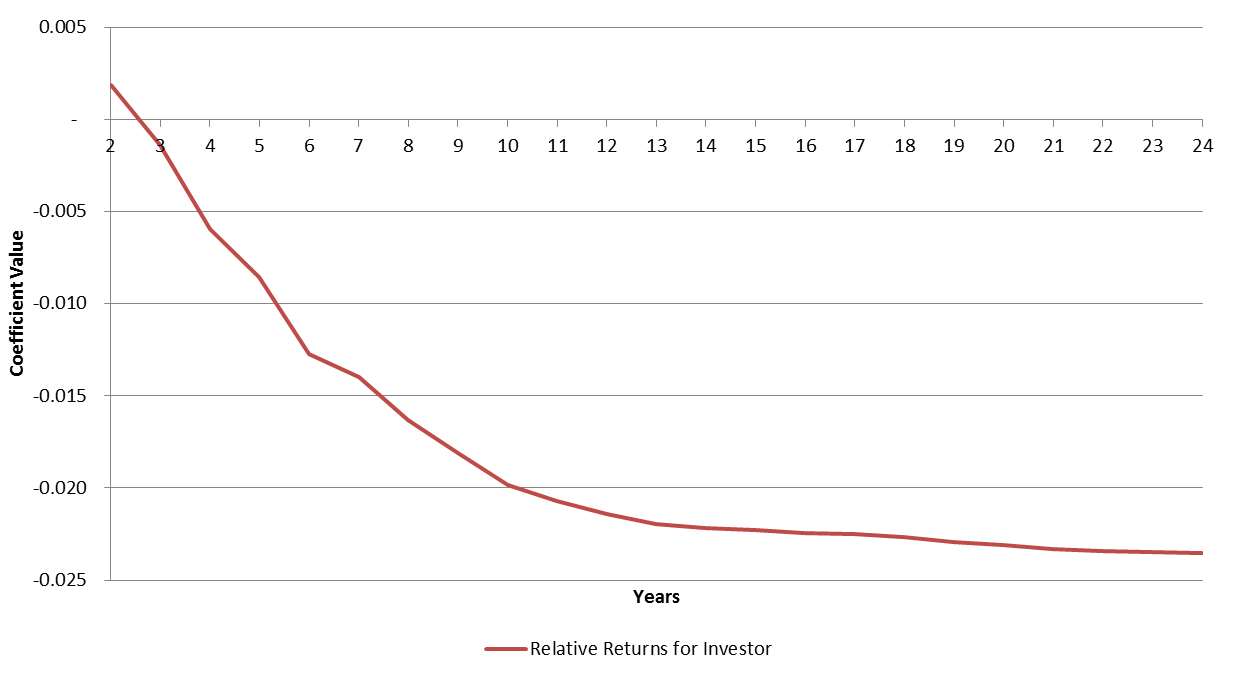
\includegraphics[width=0.9\columnwidth]{Figures/relative_returns_by_investor.png} \par
 \caption{Estimates Profile for Investors by Tenure}
 \vspace{-20pt}
 \label{fig:relative_returns_by_investor}
\end{figure} 



We see that for less than two years i.e. for the speculators type I (flippers), the returns are positive and as we increase the time between purchase and resale there are more homeowners, included in the regression, who are unlikely to have the speculative motive at the onset and therefore, we see that the returns start to become negative relative to unimproved homes. As we increase the number of years between sales further, the estimates become almost constant and converge to the overall mean. 


\subsection{Speculators Type II (Improve-and-Sell)}

% Table created by stargazer v.5.2 by Marek Hlavac, Harvard University. E-mail: hlavac at fas.harvard.edu
% Date and time: Mon, Jul 03, 2017 - 09:15:46 AM
% Requires LaTeX packages: dcolumn rotating 
\begin{table}[!htbp] \centering 
  \caption{Results for Speculator II}
  \label{tab:results_s0_investor2_da_interaction} 
  \resizebox{0.8\textwidth}{!}{
\begin{tabular}{@{\extracolsep{5pt}}lD{.}{.}{-3} D{.}{.}{-3} } 
\\[-1.8ex] 
\toprule \\[-1.8ex] 
\\[-1.8ex] & \multicolumn{2}{c}{Log(Resale Price/Purchase Price (Notional))} \\ 
\\[-1.8ex] & \multicolumn{1}{c}{(1)} & \multicolumn{1}{c}{(2)}\\ 
\midrule \\[-1.8ex] 
 DA & -0.012^{***} & -0.017^{***} \\ 
  & (0.002) & (0.002) \\ 
  %& & \\ 
 Investor & 0.004^{***} & 0.004^{***} \\ 
  & (0.001) & (0.001) \\ 
  %& & \\ 
 DA*Investor & -0.042^{***} & -0.040^{***} \\ 
  & (0.005) & (0.005) \\ 
  %& & \\ 
 MktReturn & 0.920^{***} & 0.922^{***} \\ 
  & (0.003) & (0.003) \\ 
  %& & \\ 
 Age & -0.002^{***} & -0.002^{***} \\ 
  & (0.000) & (0.000) \\ 
  %& & \\ 
 Age Squared & 0.000^{***} & 0.000^{***} \\ 
  & (0.000) & (0.000) \\ 
  %& & \\ 
 No. of beds (Resale) & 0.027^{***} &  \\ 
  & (0.001) &  \\ 
  %& & \\ 
 No. of baths (Resale) & 0.058^{***} &  \\ 
  & (0.001) &  \\ 
  %& & \\ 
 No. of cars (Resale) & 0.006^{***} &  \\ 
  & (0.000) &  \\ 
  %& & \\ 
 No. of beds (Purchase) & -0.033^{***} &  \\ 
  & (0.001) &  \\ 
  %& & \\ 
 No. of baths (Purchase) & -0.067^{***} &  \\ 
  & (0.001) &  \\ 
  %& & \\ 
 No. of cars (Purchase) & -0.016^{***} &  \\ 
  & (0.000) &  \\ 
  %& & \\ 
 Change in \# of beds &  & 0.029^{***} \\ 
  &  & (0.001) \\ 
  %& & \\ 
 Change in \# of baths &  & 0.062^{***} \\ 
  &  & (0.001) \\ 
  %& & \\ 
 Change in \# of cars &  & 0.010^{***} \\ 
  &  & (0.000) \\ 
  %& & \\ 
 Constant & 0.131^{***} & 0.078^{***} \\ 
  & (0.005) & (0.004) \\ 
  %& & \\ 
Year Fixed Effects & Yes & Yes \\ 
Location Fixed Effects & Yes & Yes \\ 
Observations & \multicolumn{1}{c}{522,826} & \multicolumn{1}{c}{522,826} \\ 
Adjusted R$^{2}$ & \multicolumn{1}{c}{0.286} & \multicolumn{1}{c}{0.284} \\ 
F Statistic & \multicolumn{1}{c}{6,757.326$^{***}$} & 

\multicolumn{1}{c}{7,391.931$^{***}$} \\ 
& \multicolumn{1}{c}{(df = 31; 522794)} & \multicolumn{1}{c}{(df = 28; 522797)} \\ 
\bottomrule \\[-1.8ex] 

\multicolumn{3}{l}{Notes: *** 0.1\% significance ** 1\% significance * 5\% significance.}\\

\multicolumn{3}{p{12cm}}{Robust standard errors are reported in parenthesis and the significance of the variables is adjusted accordingly.}\\
\end{tabular}
}

\end{table}

For speculators type II, where the homeowner carries out home improvement and then sells within 2 years of home improvement but in more than two years of purchasing\footnote{Homeowners with improved homes who sell within 2 years of purchase would invariably also belong to the group that sells within 2 years of carrying out home improvement as the home improvements are between the repeat sales. Therefore since these homeowners are already covered in speculator type I analysis, they are excluded from the investor type II analysis} - the aggregate level interaction results for the full model specifications - 1 and 2, are presented in table \ref{tab:results_s0_investor2_da_interaction}. 
If we look across speculator and non-speculator groups, for unimproved homes, returns for speculators is 0.4\% higher than non-speculators. This is consistent with the type I speculator results (0.7\%). Since the speculator group for unimproved homes in both cases is identified in the same way, i.e. time between purchase and resale is within 2 years, this is expected. Now, in case of improved homes, the returns for speculators is 3.8\% (0.004 + -0.042) and 3.6\% (0.004 + -0.040) lower than non-investor, in both models specifications, 1 and 2, respectively. All other variable coefficients are consistent with the main result.

Table \ref{tab:results_s0_investor2_da_type} presents results split by improvement types for model 1 to 6 for speculator group only. The results for carports in full model specifications 5 and 6 is 2.4\% (insignificant) and 2.8\% lower than unimproved homes. The results for duplex is positive, around 5.5\% higher than unimproved homes but it is lower than the positive returns in main results and investor type I results. For extension and alterations, the returns are lower by around 3\% than unimproved homes and this much lower returns as compared to the main results. For house/single dwelling also the returns for improved homes is below unimproved homes by around 22\% and far lower as compared to main results where the returns were lower by around 10\%. For Multiple DAs, the returns are around 5\% lower as compared to main results where returns were around 1\% lower. In case of swimming pools, the return is 1.6\% lower (weakly significant) as compared to main results where the swimming pool returns are insignificantly different from unimproved homes. Finally for verandas/pergolas, the return are 7\% lower compared to around 4\% lower in the main results. Overall we find that the returns in case of type II investors is not only worse than the type I investors but is also worse than the main results. 

These results could probably be so because who we think of as speculating on home improvements, are perhaps not speculators at all, but rather consumers. The main argument that supports this claim is that since these homeowners have purchased the property long before improving or selling, they are less likely to have had a speculative motive at the time of purchase and therefore more likely to have a consumption motive. Now, since these homeowners have a consumption motive at the time of purchase, they are also more likely to indulge in home improvement with a consumption motive. But the fact that they land up selling in less than 2 years after improvement, indicates that their improvement did not turn out as desired or the output of improvement does not serve their expected needs and therefore, they choose to sell soon after the improvement at reduced price which may explain why, in expectation, the returns for these homeowners are worst.

\newgeometry{margin=1in}
% Table created by stargazer v.5.2 by Marek Hlavac, Harvard University. E-mail: hlavac at fas.harvard.edu
% Date and time: Mon, Jul 03, 2017 - 09:57:05 AM
% Requires LaTeX packages: dcolumn rotating 
\begin{sidewaystable}[!htbp] \centering 
  \caption{Results for Speculators Type II by DA types}
  \label{tab:results_s0_investor2_da_type} 
  \resizebox{\textwidth}{!}{

\begin{threeparttable}

\begin{tabular}{@{\extracolsep{5pt}}lD{.}{.}{-3} D{.}{.}{-3} D{.}{.}{-3} D{.}{.}{-3} } 
\\[-1.8ex] 
\toprule \\[-1.8ex] 
\\[-1.8ex] & \multicolumn{4}{c}{Log(Resale Price/Purchase Price (Notional))} \\ 
\\[-1.8ex] & \multicolumn{1}{c}{(1)} & \multicolumn{1}{c}{(2)} & \multicolumn{1}{c}{(3)} & \multicolumn{1}{c}{(4)}\\ 
\midrule \\[-1.8ex] 
 Carports/Garages/Sheds & -0.027^{*} & -0.023 & -0.024 & -0.028^{*} \\ 
  & (0.016) & (0.016) & (0.016) & (0.016) \\ 
  %& & & & \\ 
 Duplex & 0.055^{**} & 0.087^{***} & 0.055^{**} & 0.059^{**} \\ 
  & (0.027) & (0.028) & (0.028) & (0.028) \\ 
  %& & & & \\ 
 Extension/Alteration & -0.034^{***} & -0.028^{***} & -0.030^{***} & -0.031^{***} \\ 
  & (0.009) & (0.009) & (0.009) & (0.009) \\ 
  %& & & & \\ 
 House/Single Dwelling & -0.229^{***} & -0.206^{***} & -0.223^{***} & -0.223^{***} \\ 
  & (0.017) & (0.017) & (0.017) & (0.017) \\ 
  %& & & & \\ 
 Multiple DA & -0.061^{***} & -0.043^{***} & -0.053^{***} & -0.057^{***} \\ 
  & (0.012) & (0.012) & (0.012) & (0.012) \\ 
  %& & & & \\ 
 Swimming Pool & -0.023^{**} & -0.012 & -0.016^{*} & -0.022^{**} \\ 
  & (0.009) & (0.009) & (0.009) & (0.009) \\ 
  %& & & & \\ 
 Verandahs/Pergolas & -0.070^{***} & -0.069^{***} & -0.070^{***} & -0.072^{***} \\ 
  & (0.007) & (0.007) & (0.007) & (0.007) \\ 
  %& & & & \\ 
 MktReturn & 0.875^{***} & 0.934^{***} & 0.936^{***} & 0.941^{***} \\ 
  & (0.009) & (0.010) & (0.010) & (0.010) \\ 
  %& & & & \\ 
 Months between sales &  & -0.002^{***} & -0.006^{***} & -0.006^{***} \\ 
  &  & (0.000) & (0.001) & (0.001) \\ 
  %& & & & \\ 
 Months between sales squared &  &  & 0.000^{***} & 0.000^{***} \\ 
  &  &  & (0.000) & (0.000) \\ 
  %& & & & \\ 
 No. of beds (resale) & 0.032^{***} & 0.032^{***} & 0.032^{***} &  \\ 
  & (0.002) & (0.002) & (0.002) &  \\ 
  %& & & & \\ 
 No. of baths (resale) & 0.061^{***} & 0.061^{***} & 0.061^{***} &  \\ 
  & (0.002) & (0.002) & (0.002) &  \\ 
  %& & & & \\ 
 No. of cars (resale) & 0.004^{***} & 0.004^{***} & 0.004^{***} &  \\ 
  & (0.001) & (0.001) & (0.001) &  \\ 
  %& & & & \\ 
 No. of beds (purchase) & -0.037^{***} & -0.037^{***} & -0.037^{***} &  \\ 
  & (0.002) & (0.002) & (0.002) &  \\ 
  %& & & & \\ 
 No. of baths (purchase) & -0.068^{***} & -0.069^{***} & -0.069^{***} &  \\ 
  & (0.002) & (0.002) & (0.002) &  \\ 
  %& & & & \\ 
 No. of cars (purchase) & -0.015^{***} & -0.015^{***} & -0.015^{***} &  \\ 
  & (0.001) & (0.001) & (0.001) &  \\ 
  %& & & & \\ 
 Change in \# of beds &  &  &  & 0.034^{***} \\ 
  &  &  &  & (0.002) \\ 
  %& & & & \\ 
 Change in \# of baths &  &  &  & 0.064^{***} \\ 
  &  &  &  & (0.002) \\ 
  %& & & & \\ 
 Change in \# of cars &  &  &  & 0.009^{***} \\ 
  &  &  &  & (0.001) \\ 
  %& & & & \\ 
 Constant & 0.082^{***} & 0.111^{***} & 0.134^{***} & 0.088^{***} \\ 
  & (0.005) & (0.006) & (0.007) & (0.007) \\ 
  %& & & & \\ 
Year Fixed Effects & Yes & Yes & Yes & Yes \\ 
Location Fixed Effects & Yes & Yes & Yes & Yes \\ 
Observations & \multicolumn{1}{c}{119,639} & \multicolumn{1}{c}{119,639} & \multicolumn{1}{c}{119,639} & \multicolumn{1}{c}{119,639} \\ 
Adjusted R$^{2}$ & \multicolumn{1}{c}{0.125} & \multicolumn{1}{c}{0.127} & \multicolumn{1}{c}{0.128} & \multicolumn{1}{c}{0.125} \\ 
F Statistic & \multicolumn{1}{c}{551.779$^{***}$ (df = 31; 119607)} & \multicolumn{1}{c}{545.483$^{***}$ (df = 32; 119606)} & \multicolumn{1}{c}{530.886$^{***}$ (df = 33; 119605)} & \multicolumn{1}{c}{572.333$^{***}$ (df = 30; 119608)} \\ 



%F Statistic & \multicolumn{1}{c}{530.034$^{***}$ (df = 27; 278396)} & \multicolumn{1}{c}{562.837$^{***}$ (df = 30; 241261)} & \multicolumn{1}{c}{512.442$^{***}$ (df = 33; 121448)} & \multicolumn{1}{c}{507.338$^{***}$ (df = 34; 121447)} & \multicolumn{1}{c}{494.641$^{***}$ (df = 35; 121446)} & \multicolumn{1}{c}{530.320$^{***}$ (df = 32; 121449)} \\ 


\bottomrule \\[-1.8ex] 

\end{tabular} 

\begin{tablenotes}[para,flushleft]
  \LARGE
      Notes: Robust standard errors are reported in parentheses, Significance of variables is adjusted accordingly. *** 0.1\% significance ** 1\% significance * 5\% significance. We have a total of 272,348 (11,046 for treatment and 261,302 for control sample) possible observation with deviation accounted for by missing data.
\end{tablenotes}    


\end{threeparttable}
}
\end{sidewaystable} 
\restoregeometry


%% Table created by stargazer v.5.2 by Marek Hlavac, Harvard University. E-mail: hlavac at fas.harvard.edu
% Date and time: Mon, Jul 03, 2017 - 11:02:16 AM
% Requires LaTeX packages: dcolumn rotating 
\begin{sidewaystable}[!p] \centering 
  \caption{Results for Investor Type I}
  \label{tab:results_s0_investor1} 
  \resizebox{\textwidth}{!}{ 
\begin{tabular}{@{\extracolsep{5pt}}lD{.}{.}{-3} D{.}{.}{-3} D{.}{.}{-3} D{.}{.}{-3} D{.}{.}{-3} D{.}{.}{-3} D{.}{.}{-3} D{.}{.}{-3} } 
\\[-1.8ex] 
\toprule \\[-1.8ex] 
\\[-1.8ex] & \multicolumn{8}{c}{Log(Resale Price/Purchase Price (Notional))} \\ 
\\[-1.8ex] & \multicolumn{1}{c}{(1)} & \multicolumn{1}{c}{(2)} & \multicolumn{1}{c}{(3)} & \multicolumn{1}{c}{(4)} & \multicolumn{1}{c}{(5)} & \multicolumn{1}{c}{(6)} & \multicolumn{1}{c}{(7)} & \multicolumn{1}{c}{(8)}\\ 
\midrule \\[-1.8ex] 
  DA &  &  &  &  &  &  & -0.021^{***} & -0.025^{***} \\ 
  &  &  &  &  &  &  & (0.002) & (0.002) \\ 
  & & & & & & & & \\ 
 Investor I &  &  &  &  &  &  & 0.007^{***} & 0.007^{***} \\ 
  &  &  &  &  &  &  & (0.001) & (0.001) \\ 
  & & & & & & & & \\
 DA*investor &  &  &  &  &  &  & 0.025^{***} & 0.026^{***} \\ 
  &  &  &  &  &  &  & (0.006) & (0.006) \\ 
  & & & & & & & & \\ 
 Carports/Garages/Sheds & -0.063^{***} & -0.049^{**} & 0.018 & 0.012 & 0.013 & 0.009 &  &  \\ 
  & (0.023) & (0.024) & (0.024) & (0.024) & (0.024) & (0.024) &  &  \\ 
  & & & & & & & & \\ 
 Duplex & 0.139^{***} & 0.087^{***} & 0.066^{***} & 0.087^{***} & 0.080^{***} & 0.082^{***} &  &  \\ 
  & (0.014) & (0.014) & (0.017) & (0.017) & (0.017) & (0.017) &  &  \\ 
  & & & & & & & & \\ 
 Extension/Alteration & 0.082^{***} & 0.048^{***} & 0.058^{***} & 0.053^{***} & 0.055^{***} & 0.054^{***} &  &  \\ 
  & (0.008) & (0.009) & (0.010) & (0.010) & (0.010) & (0.010) &  &  \\ 
  & & & & & & & & \\ 
 House/Single Dwelling & -0.111^{***} & -0.158^{***} & -0.121^{***} & -0.108^{***} & -0.110^{***} & -0.113^{***} &  &  \\ 
  & (0.012) & (0.011) & (0.017) & (0.017) & (0.017) & (0.017) &  &  \\ 
  & & & & & & & & \\ 
 Multiple\_DAs & 0.021 & -0.028^{*} & 0.016 & 0.024 & 0.024 & 0.019 &  &  \\ 
  & (0.015) & (0.015) & (0.020) & (0.021) & (0.021) & (0.020) &  &  \\ 
  & & & & & & & & \\ 
 Swimming Pool & 0.041^{***} & 0.020 & 0.011 & 0.012 & 0.013 & 0.005 &  &  \\ 
  & (0.014) & (0.014) & (0.009) & (0.009) & (0.009) & (0.009) &  &  \\ 
  & & & & & & & & \\ 
 Verandahs/Pergolas & -0.049^{***} & -0.042^{***} & 0.005 & -0.003 & -0.003 & -0.006 &  &  \\ 
  & (0.012) & (0.013) & (0.012) & (0.012) & (0.012) & (0.012) &  &  \\ 
  & & & & & & & & \\ 
 MktReturn & 0.796^{***} & 0.829^{***} & 0.868^{***} & 0.931^{***} & 0.933^{***} & 0.938^{***} & 0.921^{***} & 0.923^{***} \\ 
  & (0.009) & (0.009) & (0.009) & (0.010) & (0.010) & (0.010) & (0.003) & (0.003) \\ 
  & & & & & & & & \\ 
 Age &  &  &  & -0.003^{***} & -0.006^{***} & -0.006^{***} & -0.002^{***} & -0.002^{***} \\ 
  &  &  &  & (0.000) & (0.001) & (0.001) & (0.000) & (0.000) \\ 
  & & & & & & & & \\ 
 Age Squared &  &  &  &  & 0.000^{***} & 0.000^{***} & 0.000^{***} & 0.000^{***} \\ 
  &  &  &  &  & (0.000) & (0.000) & (0.000) & (0.000) \\ 
  & & & & & & & & \\ 
 No. of beds (Resale) &  & 0.020^{***} & 0.031^{***} & 0.031^{***} & 0.031^{***} &  & 0.026^{***} &  \\ 
  &  & (0.001) & (0.002) & (0.002) & (0.002) &  & (0.001) &  \\ 
  & & & & & & & & \\ 
 No. of baths (Resale) &  & 0.050^{***} & 0.058^{***} & 0.059^{***} & 0.059^{***} &  & 0.058^{***} &  \\ 
  &  & (0.002) & (0.002) & (0.002) & (0.002) &  & (0.001) &  \\ 
  & & & & & & & & \\ 
 No. of cars (Resale) &  & -0.010^{***} & 0.004^{***} & 0.004^{***} & 0.004^{***} &  & 0.006^{***} &  \\ 
  &  & (0.001) & (0.001) & (0.001) & (0.001) &  & (0.000) &  \\ 
  & & & & & & & & \\ 
 No. of beds (Purchase) &  &  & -0.035^{***} & -0.035^{***} & -0.035^{***} &  & -0.033^{***} &  \\ 
  &  &  & (0.002) & (0.002) & (0.002) &  & (0.001) &  \\ 
  & & & & & & & & \\ 
 No. of baths (Purchase) &  &  & -0.067^{***} & -0.068^{***} & -0.068^{***} &  & -0.067^{***} &  \\ 
  &  &  & (0.002) & (0.002) & (0.002) &  & (0.001) &  \\ 
  & & & & & & & & \\ 
 No. of cars (Purchase) &  &  & -0.015^{***} & -0.015^{***} & -0.015^{***} &  & -0.016^{***} &  \\ 
  &  &  & (0.001) & (0.001) & (0.001) &  & (0.000) &  \\ 
  & & & & & & & & \\ 
 Change in \# of beds &  &  &  &  &  & 0.033^{***} &  & 0.029^{***} \\ 
  &  &  &  &  &  & (0.002) &  & (0.001) \\ 
  & & & & & & & & \\ 
 Change in \# of beds &  &  &  &  &  & 0.062^{***} &  & 0.062^{***} \\ 
  &  &  &  &  &  & (0.002) &  & (0.001) \\ 
  & & & & & & & & \\ 
 Change in \# of beds &  &  &  &  &  & 0.009^{***} &  & 0.010^{***} \\ 
  &  &  &  &  &  & (0.001) &  & (0.000) \\ 
  & & & & & & & & \\ 
  Constant & 0.059^{***} & -0.083^{***} & 0.054^{***} & 0.088^{***} & 0.105^{***} & 0.061^{***} & 0.126^{***} & 0.075^{***} \\ 
  & (0.007) & (0.008) & (0.010) & (0.010) & (0.011) & (0.011) & (0.005) & (0.004) \\ 
  & & & & & & & & \\ 
Year Fixed Effects & Yes & Yes & Yes & Yes & Yes & Yes &  &  \\ 
Location Fixed Effects & Yes & Yes & Yes & Yes & Yes & Yes &  &  \\ 
Observations & \multicolumn{1}{c}{271,575} & \multicolumn{1}{c}{234,902} & \multicolumn{1}{c}{119,448} & \multicolumn{1}{c}{119,448} & \multicolumn{1}{c}{119,448} & \multicolumn{1}{c}{119,448} & \multicolumn{1}{c}{525,144} & \multicolumn{1}{c}{525,144} \\ 
Adjusted R$^{2}$ & \multicolumn{1}{c}{0.046} & \multicolumn{1}{c}{0.062} & \multicolumn{1}{c}{0.120} & \multicolumn{1}{c}{0.123} & \multicolumn{1}{c}{0.123} & \multicolumn{1}{c}{0.121} & \multicolumn{1}{c}{0.285} & \multicolumn{1}{c}{0.283} \\ 
F Statistic & \multicolumn{1}{c}{488.390$^{***}$ (df = 27; 271547)} & \multicolumn{1}{c}{518.701$^{***}$ (df = 30; 234871)} & \multicolumn{1}{c}{495.690$^{***}$ (df = 33; 119414)} & \multicolumn{1}{c}{492.394$^{***}$ (df = 34; 119413)} & \multicolumn{1}{c}{479.292$^{***}$ (df = 35; 119412)} & \multicolumn{1}{c}{513.604$^{***}$ (df = 32; 119415)} & \multicolumn{1}{c}{6,761.652$^{***}$ (df = 31; 525112)} & \multicolumn{1}{c}{7,398.417$^{***}$ (df = 28; 525115)} \\ 
\bottomrule \\[-1.8ex] 
\textit{Notes:} & \multicolumn{8}{l}{Robust standard errors in parentheses. *** 0.1\% significance ** 1\% significance * 5\% significance . 10\% significance} \\ 
\end{tabular}%
}%
\end{sidewaystable} 
%% Table created by stargazer v.5.2 by Marek Hlavac, Harvard University. E-mail: hlavac at fas.harvard.edu
% Date and time: Mon, Jul 03, 2017 - 10:37:01 AM
% Requires LaTeX packages: dcolumn rotating 
\begin{sidewaystable}[!htbp] \centering 
 \caption{Results for Investor Type II}
  \label{tab:results_s0_investor2} 
  \resizebox{\textwidth}{!}{ 
\begin{tabular}{@{\extracolsep{5pt}}lD{.}{.}{-3} D{.}{.}{-3} D{.}{.}{-3} D{.}{.}{-3} D{.}{.}{-3} D{.}{.}{-3} D{.}{.}{-3} D{.}{.}{-3} } 
\\[-1.8ex] 
\toprule \\[-1.8ex] 
\\[-1.8ex] & \multicolumn{8}{c}{Log(Resale Price/Purchase Price (Notional))} \\ 
\\[-1.8ex] & \multicolumn{1}{c}{(1)} & \multicolumn{1}{c}{(2)} & \multicolumn{1}{c}{(3)} & \multicolumn{1}{c}{(4)} & \multicolumn{1}{c}{(5)} & \multicolumn{1}{c}{(6)} & \multicolumn{1}{c}{(7)} & \multicolumn{1}{c}{(8)}\\ 
\midrule \\[-1.8ex] 
 DA &  &  &  &  &  &  & -0.012^{***} & -0.017^{***} \\ 
  &  &  &  &  &  &  & (0.002) & (0.002) \\ 
  & & & & & & & & \\ 
 Investor II &  &  &  &  &  &  & 0.004^{***} & 0.004^{***} \\ 
  &  &  &  &  &  &  & (0.001) & (0.001) \\ 
  & & & & & & & & \\ 
 DA:investor\_da &  &  &  &  &  &  & -0.042^{***} & -0.040^{***} \\ 
  &  &  &  &  &  &  & (0.005) & (0.005) \\ 
  & & & & & & & & \\ 
 Carports/Garages/Sheds & -0.100^{***} & -0.079^{***} & -0.027^{*} & -0.024 & -0.024 & -0.028^{*} &  &  \\ 
  & (0.016) & (0.015) & (0.016) & (0.016) & (0.016) & (0.016) &  &  \\ 
  & & & & & & & & \\ 
 Duplex & 0.130^{***} & 0.076^{***} & 0.055^{**} & 0.087^{***} & 0.055^{**} & 0.059^{**} &  &  \\ 
  & (0.026) & (0.026) & (0.027) & (0.028) & (0.028) & (0.028) &  &  \\ 
  & & & & & & & & \\ 
 Extension/Alteration & -0.015^{**} & -0.051^{***} & -0.033^{***} & -0.028^{***} & -0.030^{***} & -0.031^{***} &  &  \\ 
  & (0.007) & (0.007) & (0.009) & (0.009) & (0.009) & (0.009) &  &  \\ 
  & & & & & & & & \\ 
 House/Single Dwelling & -0.193^{***} & -0.240^{***} & -0.229^{***} & -0.206^{***} & -0.222^{***} & -0.223^{***} &  &  \\ 
  & (0.013) & (0.013) & (0.017) & (0.017) & (0.017) & (0.017) &  &  \\ 
  & & & & & & & & \\ 
 Multiple\_DAs & -0.017^{**} & -0.048^{***} & -0.061^{***} & -0.043^{***} & -0.053^{***} & -0.058^{***} &  &  \\ 
  & (0.007) & (0.008) & (0.012) & (0.012) & (0.012) & (0.012) &  &  \\ 
  & & & & & & & & \\ 
 Swimming Pool & 0.181^{***} & 0.151^{***} & -0.023^{**} & -0.013 & -0.016^{*} & -0.023^{**} &  &  \\ 
  & (0.010) & (0.010) & (0.009) & (0.009) & (0.009) & (0.009) &  &  \\ 
  & & & & & & & & \\ 
 Verandahs/Pergolas & -0.016^{**} & -0.018^{**} & -0.070^{***} & -0.070^{***} & -0.070^{***} & -0.073^{***} &  &  \\ 
  & (0.008) & (0.008) & (0.007) & (0.007) & (0.007) & (0.007) &  &  \\ 
  & & & & & & & & \\ 
 MktReturn & 0.803^{***} & 0.835^{***} & 0.873^{***} & 0.931^{***} & 0.933^{***} & 0.938^{***} & 0.920^{***} & 0.922^{***} \\ 
  & (0.009) & (0.009) & (0.009) & (0.010) & (0.010) & (0.010) & (0.003) & (0.003) \\ 
  & & & & & & & & \\ 
 Age &  &  &  & -0.002^{***} & -0.006^{***} & -0.006^{***} & -0.002^{***} & -0.002^{***} \\ 
  &  &  &  & (0.000) & (0.001) & (0.001) & (0.000) & (0.000) \\ 
  & & & & & & & & \\ 
 Age Squared &  &  &  &  & 0.000^{***} & 0.000^{***} & 0.000^{***} & 0.000^{***} \\ 
  &  &  &  &  & (0.000) & (0.000) & (0.000) & (0.000) \\ 
  & & & & & & & & \\ 
 No. of beds (Resale) &  & 0.021^{***} & 0.032^{***} & 0.032^{***} & 0.032^{***} &  & 0.027^{***} &  \\ 
  &  & (0.001) & (0.002) & (0.002) & (0.002) &  & (0.001) &  \\ 
  & & & & & & & & \\ 
 No. of baths (Resale) &  & 0.052^{***} & 0.060^{***} & 0.060^{***} & 0.060^{***} &  & 0.058^{***} &  \\ 
  &  & (0.002) & (0.002) & (0.002) & (0.002) &  & (0.001) &  \\ 
  & & & & & & & & \\ 
 No. of cars (Resale) &  & -0.009^{***} & 0.004^{***} & 0.005^{***} & 0.005^{***} &  & 0.006^{***} &  \\ 
  &  & (0.001) & (0.001) & (0.001) & (0.001) &  & (0.000) &  \\ 
  & & & & & & & & \\ 
 No. of beds (Purchase) &  &  & -0.036^{***} & -0.036^{***} & -0.036^{***} &  & -0.033^{***} &  \\ 
  &  &  & (0.002) & (0.002) & (0.002) &  & (0.001) &  \\ 
  & & & & & & & & \\ 
 No. of baths (Purchase) &  &  & -0.068^{***} & -0.068^{***} & -0.068^{***} &  & -0.067^{***} &  \\ 
  &  &  & (0.002) & (0.002) & (0.002) &  & (0.001) &  \\ 
  & & & & & & & & \\ 
 No. of cars (Purchase) &  &  & -0.015^{***} & -0.015^{***} & -0.015^{***} &  & -0.016^{***} &  \\ 
  &  &  & (0.001) & (0.001) & (0.001) &  & (0.000) &  \\ 
  & & & & & & & & \\ 
 Change in \# of beds &  &  &  &  &  & 0.034^{***} &  & 0.029^{***} \\ 
  &  &  &  &  &  & (0.002) &  & (0.001) \\ 
  & & & & & & & & \\ 
 Change in \# of baths &  &  &  &  &  & 0.064^{***} &  & 0.062^{***} \\ 
  &  &  &  &  &  & (0.002) &  & (0.001) \\ 
  & & & & & & & & \\ 
 Change in \# of cars &  &  &  &  &  & 0.009^{***} &  & 0.010^{***} \\ 
  &  &  &  &  &  & (0.001) &  & (0.000) \\ 
  & & & & & & & & \\ 
 Constant & 0.060^{***} & -0.085^{***} & 0.057^{***} & 0.088^{***} & 0.111^{***} & 0.065^{***} & 0.131^{***} & 0.078^{***} \\ 
  & (0.007) & (0.008) & (0.010) & (0.010) & (0.011) & (0.011) & (0.005) & (0.004) \\ 
  & & & & & & & & \\ 
Year Fixed Effects & Yes & Yes & Yes & Yes & Yes & Yes &  &  \\ 
Location Fixed Effects & Yes & Yes & Yes & Yes & Yes & Yes &  &  \\ 
Observations & \multicolumn{1}{c}{278,424} & \multicolumn{1}{c}{241,292} & \multicolumn{1}{c}{121,482} & \multicolumn{1}{c}{121,482} & \multicolumn{1}{c}{121,482} & \multicolumn{1}{c}{121,482} & \multicolumn{1}{c}{522,826} & \multicolumn{1}{c}{522,826} \\ 
Adjusted R$^{2}$ & \multicolumn{1}{c}{0.049} & \multicolumn{1}{c}{0.065} & \multicolumn{1}{c}{0.122} & \multicolumn{1}{c}{0.124} & \multicolumn{1}{c}{0.125} & \multicolumn{1}{c}{0.122} & \multicolumn{1}{c}{0.286} & \multicolumn{1}{c}{0.284} \\ 
F Statistic & \multicolumn{1}{c}{530.034$^{***}$ (df = 27; 278396)} & \multicolumn{1}{c}{562.837$^{***}$ (df = 30; 241261)} & \multicolumn{1}{c}{512.442$^{***}$ (df = 33; 121448)} & \multicolumn{1}{c}{507.338$^{***}$ (df = 34; 121447)} & \multicolumn{1}{c}{494.641$^{***}$ (df = 35; 121446)} & \multicolumn{1}{c}{530.320$^{***}$ (df = 32; 121449)} & \multicolumn{1}{c}{6,757.326$^{***}$ (df = 31; 522794)} & \multicolumn{1}{c}{7,391.931$^{***}$ (df = 28; 522797)} \\ 
\bottomrule \\[-1.8ex] 
\textit{Notes:} & \multicolumn{8}{l}{Robust standard errors in parentheses. *** 0.1\% significance ** 1\% significance * 5\% significance . 10\% significance} \\ 
\end{tabular}
}%
\end{sidewaystable} 

%% Table generated by Excel2LaTeX from sheet 'Table and descriptive'
\begin{table}[!ht]
  \centering
  \caption{Variable Descriptions and Sample Statistics - Repeat Sales Markup Model}
 \resizebox{0.9\textwidth}{!}{
    \begin{tabu} to \textwidth {X[1.7,l]X[3,l]X[0.7,c]X[0.9,c]}
   \toprule
    Name  & Description & Mean  & Std. deviation \\
    \midrule
    No. of obs. &       & 56,665 &  \\
    Sales Price & Nominal contract price of the house &       &  \\
    Previous Sale Price & Sale Price prior to DA & 447,549 & 492,464 \\
    Current Sale Price & Sale Price at subsequent sale post DA (Repeat Sale) & 901,225 & 867,079 \\
    Expected Current Sale Price & Previous sale price appreciated by the growth rate of corresponding SSD area hedonic Index (monthly) between the period from time of previous sale to time of current sale & 697,276 & 757,545 \\
    Avg. SSD Hedonic Index growth rate & Annual average growth rate of statistical sub-division specific Hedonic Index for property type 'House' for the period 1990 - 2016 & 0.073 & 0.048 \\
    DA cost & Cost of developments as reported in development applications & 104,417 & 169,189 \\
    DA cost at time of current sale & Cost of development indexed by CPI to the time of current sale & 115,679 & 186,725 \\
    CPI   & Annual average growth rate of CPI for period 2004 - 2016 & 0.025 & 0.009 \\
    Markup & Difference between the Current Sale Price and the Expected Current Sale Price & 214,403 & 522,817 \\
    Age of DA at current sale & Number of months between the DA date and the current sale date & 48    & 31 \\
    Trend & Time trend at point of current sale, 2004-2016 &       &  \\
    DA Types & Duplex, Extension/Alteration, Garages/Sheds \& Carports,House/Single Dwelling, Multiple DA, Swimming Pool and Verandahs \& Pergolas &       &  \\
    DA cost:DA types & Interaction terms between DA cost and different DA types &       &  \\
    Period & Pre-2004 (DA data not available), Post-2004 (DA data available) &       &  \\
    DA cost:Period & Interaction term between DA cost and Period &       &  \\
    \bottomrule
    \end{tabu}%
}
  \label{tab:markup_model_ds}%
\end{table}%

%
% Table created by stargazer v.5.2 by Marek Hlavac, Harvard University. E-mail: hlavac at fas.harvard.edu
% Date and time: Tue, Feb 28, 2017 - 5:44:45 PM
% Requires LaTeX packages: dcolumn rotating 
\begin{sidewaystable}[ph!] \centering 
  \caption{Repeat Sales Markup Model Results} 
  \label{tab:markup_model} 
\resizebox{\columnwidth}{!}{
\begin{tabular}{@{\extracolsep{5pt}}lD{.}{.}{-3} D{.}{.}{-3} D{.}{.}{-3} D{.}{.}{-3} D{.}{.}{-3} D{.}{.}{-3} D{.}{.}{-3} D{.}{.}{-3} D{.}{.}{-3} } 
\\[-1.8ex]\hline 
\hline \\[-1.8ex] 
\\[-1.8ex] & \multicolumn{9}{c}{Markup} \\ 
\\[-1.8ex] & \multicolumn{1}{c}{(1)} & \multicolumn{1}{c}{(2)} & \multicolumn{1}{c}{(3)} & \multicolumn{1}{c}{(4)} & \multicolumn{1}{c}{(5)} & \multicolumn{1}{c}{(6)} & \multicolumn{1}{c}{(7)} & \multicolumn{1}{c}{(8)} & \multicolumn{1}{c}{(9)}\\ 
\hline \\[-1.8ex] 
 DA cost (CPI-indexed to current sale) & 0.810^{***} & 0.808^{***} & 0.819^{***} & 0.647^{***} & 0.918^{***} & 0.649^{***} & 0.617^{***} & 0.750^{***} & 0.723^{***} \\ 
  & (0.015) & (0.015) & (0.015) & (0.015) & (0.020) & (0.017) & (0.017) & (0.019) & (0.020) \\ 
  & & & & & & & & & \\ 
 Age of DA at current sale &  & -305.100^{***} & -250.271^{***} & -139.164^{***} & -1,073.320^{***} & -825.410^{***} & -881.247^{***} & -1,015.461^{***} & -977.560^{***} \\ 
  &  & (49.972) & (50.232) & (50.248) & (98.545) & (92.769) & (95.454) & (92.321) & (94.220) \\ 
  & & & & & & & & & \\ 
 Trend &  &  & -21.025^{***} & -27.373^{***} & -23.573^{***} & -22.844^{***} & -23.392^{***} & -23.497^{***} & -26.462^{***} \\ 
  &  &  & (2.113) & (2.127) & (3.334) & (3.220) & (3.235) & (3.187) & (3.201) \\ 
  & & & & & & & & & \\ 
 No. of beds (current)  &  &  &  & -8,984.272^{***} &  & 16,032.400^{***} & 25,812.410^{***} & 22,940.730^{***} & 31,461.810^{***} \\ 
  &  &  &  & (2,945.276) &  & (4,285.974) & (4,382.804) & (4,297.495) & (4,386.152) \\ 
  & & & & & & & & & \\ 
 No. of baths (current) &  &  &  & 138,497.400^{***} &  & 180,753.800^{***} & 174,515.300^{***} & 182,550.800^{***} & 172,715.800^{***} \\ 
  &  &  &  & (3,270.397) &  & (4,505.380) & (4,648.389) & (4,644.713) & (4,709.690) \\ 
  & & & & & & & & & \\ 
 No. of cars (current) &  &  &  & 11,811.890^{***} &  & 21,082.820^{***} & 21,603.060^{***} & 14,506.580^{***} & 15,113.380^{***} \\ 
  &  &  &  & (1,921.746) &  & (2,969.291) & (2,987.570) & (2,962.428) & (2,972.544) \\ 
  & & & & & & & & & \\ 
 No. of beds (previous) &  &  &  &  & -16,092.970^{***} & -47,352.430^{***} & -48,071.870^{***} & -57,697.150^{***} & -56,972.110^{***} \\ 
  &  &  &  &  & (4,505.716) & (4,624.519) & (4,684.481) & (4,756.464) & (4,762.582) \\ 
  & & & & & & & & & \\ 
 No. of baths (previous) &  &  &  &  & -44,448.100^{***} & -126,006.500^{***} & -125,474.000^{***} & -138,997.500^{***} & -139,850.200^{***} \\ 
  &  &  &  &  & (5,571.672) & (5,718.278) & (5,715.206) & (5,820.079) & (5,800.077) \\ 
  & & & & & & & & & \\ 
 No. of cars (previous) &  &  &  &  & -18,694.240^{***} & -30,888.620^{***} & -31,798.140^{***} & -29,931.560^{***} & -31,193.450^{***} \\ 
  &  &  &  &  & (3,771.921) & (3,847.073) & (3,855.981) & (3,782.164) & (3,789.165) \\ 
  & & & & & & & & & \\ 
 Constant & 34,322.190 & 45,099.040 & 385,703.800^{***} & 211,022.700^{***} & 624,965.200^{***} & 385,005.400^{***} & 358,019.400^{***} & 429,961.800^{***} & 486,114.800^{***} \\ 
  & (36,658.560) & (36,689.320) & (50,159.620) & (50,312.400) & (68,107.780) & (52,281.540) & (53,052.470) & (64,661.180) & (65,342.940) \\ 
  & & & & & & & & & \\ 
Fixed Effects - DA & Yes & Yes & Yes & Yes & Yes & No & No & Yes & Yes \\ 
Fixed Effects - State & Yes & Yes & Yes & Yes & Yes & No & Yes & No & Yes \\ 
Observations & \multicolumn{1}{c}{56,664} & \multicolumn{1}{c}{56,664} & \multicolumn{1}{c}{56,664} & \multicolumn{1}{c}{53,586} & \multicolumn{1}{c}{20,533} & \multicolumn{1}{c}{20,523} & \multicolumn{1}{c}{20,523} & \multicolumn{1}{c}{20,523} & \multicolumn{1}{c}{20,523} \\ 
Adjusted R$^{2}$ & \multicolumn{1}{c}{0.121} & \multicolumn{1}{c}{0.121} & \multicolumn{1}{c}{0.123} & \multicolumn{1}{c}{0.158} & \multicolumn{1}{c}{0.242} & \multicolumn{1}{c}{0.268} & \multicolumn{1}{c}{0.273} & \multicolumn{1}{c}{0.298} & \multicolumn{1}{c}{0.303} \\ 
\hline \\[-1.8ex] 
\textit{Notes:} & \multicolumn{9}{l}{$^{***}$Significant at the 1 percent level.} \\ 
 & \multicolumn{9}{l}{$^{**}$Significant at the 5 percent level.} \\ 
 & \multicolumn{9}{l}{$^{*}$Significant at the 10 percent level.} \\ 
\end{tabular} 
}
\end{sidewaystable} 
%
% Table created by stargazer v.5.2 by Marek Hlavac, Harvard University. E-mail: hlavac at fas.harvard.edu
% Date and time: Tue, Mar 14, 2017 - 2:11:30 PM
% Requires LaTeX packages: dcolumn rotating 
\begin{sidewaystable}[!htbp] \centering 
  \caption{Repeat Sales Markup Model Results with DA type Interaction effect} 
  \label{} 
\resizebox{\columnwidth}{!}{
\begin{tabular}{@{\extracolsep{5pt}}lD{.}{.}{-3} D{.}{.}{-3} D{.}{.}{-3} D{.}{.}{-3} D{.}{.}{-3} D{.}{.}{-3} D{.}{.}{-3} D{.}{.}{-3} D{.}{.}{-3} } 
\\[-1.8ex]\hline 
\hline \\[-1.8ex] 
\\[-1.8ex] & \multicolumn{9}{c}{markup} \\ 
\\[-1.8ex] & \multicolumn{1}{c}{(1)} & \multicolumn{1}{c}{(2)} & \multicolumn{1}{c}{(3)} & \multicolumn{1}{c}{(4)} & \multicolumn{1}{c}{(5)} & \multicolumn{1}{c}{(6)} & \multicolumn{1}{c}{(7)} & \multicolumn{1}{c}{(8)} & \multicolumn{1}{c}{(9)}\\ 
\hline \\[-1.8ex] 
 Age of DA at current sale &  & -278.207^{***} & -228.522^{***} & -114.859^{**} & -1,017.308^{***} & -926.209^{***} & -919.618^{***} & -985.974^{***} & -936.101^{***} \\ 
  &  & (49.939) & (50.194) & (50.229) & (97.634) & (91.166) & (93.492) & (91.785) & (93.638) \\ 
  & & & & & & & & & \\ 
 Trend &  &  & -19.402^{***} & -25.894^{***} & -21.303^{***} & -20.487^{***} & -22.088^{***} & -21.438^{***} & -24.541^{***} \\ 
  &  &  & (2.111) & (2.125) & (3.306) & (3.155) & (3.171) & (3.169) & (3.184) \\ 
  & & & & & & & & & \\ 
 No. of beds (current) &  &  &  & -8,486.514^{***} &  & 16,078.890^{***} & 22,741.680^{***} & 22,346.240^{***} & 30,677.570^{***} \\ 
  &  &  &  & (2,939.617) &  & (4,198.741) & (4,294.966) & (4,268.508) & (4,356.147) \\ 
  & & & & & & & & & \\ 
 No. of baths (current) &  &  &  & 137,390.800^{***} &  & 165,238.500^{***} & 156,401.700^{***} & 174,683.300^{***} & 164,859.100^{***} \\ 
  &  &  &  & (3,266.901) &  & (4,484.147) & (4,611.339) & (4,639.245) & (4,702.069) \\ 
  & & & & & & & & & \\ 
 No. of cars (current) &  &  &  & 11,747.180^{***} &  & 15,212.900^{***} & 16,075.650^{***} & 14,532.850^{***} & 14,971.470^{***} \\ 
  &  &  &  & (1,917.938) &  & (2,927.141) & (2,942.810) & (2,940.585) & (2,950.792) \\ 
  & & & & & & & & & \\ 
 No. of beds (previous) &  &  &  &  & -16,036.890^{***} & -45,361.840^{***} & -43,563.950^{***} & -56,070.020^{***} & -55,190.200^{***} \\ 
  &  &  &  &  & (4,462.086) & (4,553.879) & (4,602.348) & (4,727.111) & (4,732.390) \\ 
  & & & & & & & & & \\ 
 No. of baths (previous) &  &  &  &  & -39,731.700^{***} & -119,194.600^{***} & -117,852.100^{***} & -130,994.500^{***} & -131,793.600^{***} \\ 
  &  &  &  &  & (5,530.092) & (5,633.362) & (5,631.746) & (5,806.006) & (5,786.307) \\ 
  & & & & & & & & & \\ 
 No. of cars (previous) &  &  &  &  & -18,905.330^{***} & -29,162.650^{***} & -29,840.450^{***} & -29,558.540^{***} & -30,963.570^{***} \\ 
  &  &  &  &  & (3,732.240) & (3,755.655) & (3,766.212) & (3,754.057) & (3,760.974) \\ 
  & & & & & & & & & \\ 
 DA cost:DA Type-Carports & 0.927 & 0.838 & 0.868 & -1.024 & 1.813 & -0.591 & -0.423 & 0.637 & 0.458 \\ 
  & (4.066) & (4.065) & (4.062) & (4.018) & (4.429) & (2.382) & (2.377) & (4.259) & (4.244) \\ 
  & & & & & & & & & \\ 
 DA cost:DA Type-Duplex & -0.001 & 0.002 & 0.032 & 0.018 & 0.053 & -0.207^{***} & -0.230^{***} & 0.106 & 0.085 \\ 
  & (0.073) & (0.073) & (0.073) & (0.071) & (0.085) & (0.035) & (0.035) & (0.082) & (0.082) \\ 
  & & & & & & & & & \\ 
 DA cost:DA Type-Extension/Alteration & 0.657^{***} & 0.662^{***} & 0.679^{***} & 0.495^{***} & 0.764^{***} & 0.527^{***} & 0.462^{***} & 0.655^{***} & 0.624^{***} \\ 
  & (0.041) & (0.041) & (0.041) & (0.041) & (0.048) & (0.039) & (0.039) & (0.046) & (0.046) \\ 
  & & & & & & & & & \\ 
 DA cost:DA Type-Garages/Sheds & 0.023 & 0.028 & 0.068 & -0.328 & 0.301 & -0.210 & -0.201 & 0.197 & 0.100 \\ 
  & (1.535) & (1.534) & (1.533) & (1.500) & (1.593) & (0.971) & (0.971) & (1.532) & (1.526) \\ 
  & & & & & & & & & \\ 
 DA cost:DA Type-House/Single Dwelling & 0.878^{***} & 0.880^{***} & 0.890^{***} & 0.694^{***} & 1.105^{***} & 0.779^{***} & 0.739^{***} & 0.876^{***} & 0.860^{***} \\ 
  & (0.027) & (0.027) & (0.027) & (0.027) & (0.037) & (0.023) & (0.023) & (0.036) & (0.036) \\ 
  & & & & & & & & & \\ 
 DA cost:DA Type-Multiple\_da & 0.936^{***} & 0.930^{***} & 0.936^{***} & 0.771^{***} & 1.195^{***} & 1.036^{***} & 1.017^{***} & 0.996^{***} & 0.961^{***} \\ 
  & (0.021) & (0.021) & (0.021) & (0.021) & (0.031) & (0.024) & (0.024) & (0.030) & (0.030) \\ 
  & & & & & & & & & \\ 
 DA cost:DA Type-Pergolas & -2.467^{***} & -2.410^{***} & -2.410^{***} & -3.146^{***} & -3.331^{***} & -0.910 & 0.040 & -3.659^{***} & -4.088^{***} \\ 
  & (0.738) & (0.738) & (0.738) & (0.735) & (1.132) & (0.674) & (0.694) & (1.088) & (1.085) \\ 
  & & & & & & & & & \\ 
 DA cost:DA Type-Swimming Pool & 0.205^{***} & 0.204^{***} & 0.229^{***} & 0.109^{*} & 0.026 & 0.069 & 0.070 & 0.016 & 0.002 \\ 
  & (0.068) & (0.068) & (0.068) & (0.066) & (0.061) & (0.058) & (0.058) & (0.059) & (0.059) \\ 
  & & & & & & & & & \\ 
 DA cost:DA Type-Verandahs & -1.024^{**} & -0.961^{**} & -0.876^{*} & -1.314^{***} & -0.487 & -0.349 & -0.947^{*} & -0.910 & -1.152 \\ 
  & (0.485) & (0.485) & (0.485) & (0.485) & (0.783) & (0.512) & (0.521) & (0.752) & (0.750) \\ 
  & & & & & & & & & \\ 
 Constant & 32,060.880 & 43,090.540 & 357,188.900^{***} & 208,926.500^{***} & 566,077.100^{***} & 381,429.300^{***} & 398,146.300^{***} & 394,336.000^{***} & 455,782.000^{***} \\ 
  & (66,593.810) & (66,605.590) & (74,818.570) & (74,109.940) & (88,989.880) & (51,057.300) & (51,873.560) & (84,933.770) & (85,458.390) \\ 
  & & & & & & & & & \\ 
DA Type Fixed Effects & Yes & Yes & Yes & Yes & Yes & No & No & Yes & Yes \\ 
State Fixed Effects & Yes & Yes & Yes & Yes & Yes & No & Yes & No & Yes \\ 
Observations & \multicolumn{1}{c}{56,664} & \multicolumn{1}{c}{56,664} & \multicolumn{1}{c}{56,664} & \multicolumn{1}{c}{53,586} & \multicolumn{1}{c}{20,533} & \multicolumn{1}{c}{20,523} & \multicolumn{1}{c}{20,523} & \multicolumn{1}{c}{20,523} & \multicolumn{1}{c}{20,523} \\ 
Adjusted R$^{2}$ & \multicolumn{1}{c}{0.125} & \multicolumn{1}{c}{0.126} & \multicolumn{1}{c}{0.127} & \multicolumn{1}{c}{0.162} & \multicolumn{1}{c}{0.258} & \multicolumn{1}{c}{0.305} & \multicolumn{1}{c}{0.309} & \multicolumn{1}{c}{0.308} & \multicolumn{1}{c}{0.314} \\ 
\hline \\[-1.8ex] 
\textit{Notes:} & \multicolumn{9}{l}{$^{***}$Significant at the 1 percent level.} \\ 
 & \multicolumn{9}{l}{$^{**}$Significant at the 5 percent level.} \\ 
 & \multicolumn{9}{l}{$^{*}$Significant at the 10 percent level.} \\ 
\end{tabular} 
}
\end{sidewaystable} 

%
% Table created by stargazer v.5.2 by Marek Hlavac, Harvard University. E-mail: hlavac at fas.harvard.edu
% Date and time: Wed, Mar 15, 2017 - 2:15:51 PM
% Requires LaTeX packages: dcolumn rotating 
\begin{sidewaystable}[!htbp] \centering 
  \caption{Repeat Sales Markup Model Results with interaction effects for DA types} 
  \label{} 
  \resizebox{\columnwidth}{!}{
\begin{tabular}{@{\extracolsep{5pt}}lD{.}{.}{-3} D{.}{.}{-3} D{.}{.}{-3} D{.}{.}{-3} D{.}{.}{-3} D{.}{.}{-3} D{.}{.}{-3} D{.}{.}{-3} D{.}{.}{-3} } 
\\[-1.8ex]\hline 
\hline \\[-1.8ex] 
\\[-1.8ex] & \multicolumn{9}{c}{markup} \\ 
\\[-1.8ex] & \multicolumn{1}{c}{(1)} & \multicolumn{1}{c}{(2)} & \multicolumn{1}{c}{(3)} & \multicolumn{1}{c}{(4)} & \multicolumn{1}{c}{(5)} & \multicolumn{1}{c}{(6)} & \multicolumn{1}{c}{(7)} & \multicolumn{1}{c}{(8)} & \multicolumn{1}{c}{(9)}\\ 
\hline \\[-1.8ex] 
 Age of DA at current sale &  & -275.436^{***} & -225.884^{***} & -113.268^{**} & -1,010.731^{***} & -930.907^{***} & -918.490^{***} & -986.079^{***} & -931.338^{***} \\ 
  &  & (49.920) & (50.181) & (50.213) & (97.636) & (90.931) & (93.477) & (91.463) & (93.626) \\ 
  & & & & & & & & & \\ 
 Trend &  &  & -19.181^{***} & -25.747^{***} & -20.863^{***} & -20.482^{***} & -21.995^{***} & -21.354^{***} & -24.212^{***} \\ 
  &  &  & (2.110) & (2.123) & (3.305) & (3.155) & (3.169) & (3.168) & (3.184) \\ 
  & & & & & & & & & \\ 
 No. of beds (current) &  &  &  & -8,508.153^{***} &  & 16,080.450^{***} & 22,631.080^{***} & 22,267.690^{***} & 30,372.830^{***} \\ 
  &  &  &  & (2,939.632) &  & (4,198.589) & (4,293.893) & (4,266.664) & (4,356.382) \\ 
  & & & & & & & & & \\ 
 No. of baths (current) &  &  &  & 137,444.900^{***} &  & 165,392.600^{***} & 156,430.600^{***} & 174,676.600^{***} & 165,259.500^{***} \\ 
  &  &  &  & (3,266.274) &  & (4,478.575) & (4,611.176) & (4,638.697) & (4,701.261) \\ 
  & & & & & & & & & \\ 
 No. of cars (current) &  &  &  & 11,767.520^{***} &  & 15,229.430^{***} & 16,090.100^{***} & 14,525.090^{***} & 15,119.740^{***} \\ 
  &  &  &  & (1,917.887) &  & (2,926.058) & (2,942.086) & (2,940.221) & (2,950.954) \\ 
  & & & & & & & & & \\ 
 No. of beds (previous) &  &  &  &  & -15,693.980^{***} & -45,538.760^{***} & -43,462.990^{***} & -56,160.040^{***} & -54,877.430^{***} \\ 
  &  &  &  &  & (4,462.304) & (4,546.743) & (4,601.497) & (4,722.785) & (4,731.885) \\ 
  & & & & & & & & & \\ 
 No. of baths (previous) &  &  &  &  & -40,006.350^{***} & -119,214.100^{***} & -117,965.700^{***} & -130,978.100^{***} & -132,185.500^{***} \\ 
  &  &  &  &  & (5,531.359) & (5,633.025) & (5,630.790) & (5,805.204) & (5,786.303) \\ 
  & & & & & & & & & \\ 
 No. of cars (previous) &  &  &  &  & -18,682.220^{***} & -29,112.650^{***} & -29,792.940^{***} & -29,579.820^{***} & -30,852.550^{***} \\ 
  &  &  &  &  & (3,732.902) & (3,754.629) & (3,765.501) & (3,752.742) & (3,761.355) \\ 
  & & & & & & & & & \\ 

 DA cost:Duplex & -0.000 & 0.003 & 0.033 & 0.018 & 0.054 & -0.206^{***} & -0.230^{***} & 0.106 & 0.086 \\ 
  & (0.073) & (0.073) & (0.073) & (0.071) & (0.085) & (0.035) & (0.035) & (0.082) & (0.082) \\ 
  & & & & & & & & & \\ 
 DA cost:Extensions/Alterations & 0.658^{***} & 0.662^{***} & 0.679^{***} & 0.494^{***} & 0.764^{***} & 0.528^{***} & 0.462^{***} & 0.655^{***} & 0.624^{***} \\ 
  & (0.041) & (0.041) & (0.041) & (0.041) & (0.048) & (0.039) & (0.039) & (0.046) & (0.046) \\ 
  & & & & & & & & & \\ 
 DA cost:Garages/Sheds \& Carports & 0.121 & 0.111 & 0.145 & -0.417 & 0.429 & -0.247 & -0.245 & 0.261 & 0.134 \\ 
  & (1.435) & (1.435) & (1.434) & (1.405) & (1.498) & (0.907) & (0.908) & (1.440) & (1.435) \\ 
  & & & & & & & & & \\ 
 DA cost:House/Single Dwelling & 0.878^{***} & 0.880^{***} & 0.889^{***} & 0.694^{***} & 1.104^{***} & 0.779^{***} & 0.740^{***} & 0.876^{***} & 0.858^{***} \\ 
  & (0.027) & (0.027) & (0.027) & (0.027) & (0.037) & (0.023) & (0.023) & (0.036) & (0.036) \\ 
  & & & & & & & & & \\ 
 DA cost:Multiple\_DAs & 0.936^{***} & 0.930^{***} & 0.937^{***} & 0.771^{***} & 1.198^{***} & 1.036^{***} & 1.016^{***} & 0.996^{***} & 0.963^{***} \\ 
  & (0.021) & (0.021) & (0.021) & (0.021) & (0.031) & (0.024) & (0.024) & (0.030) & (0.030) \\ 
  & & & & & & & & & \\ 
 DA cost:Swimming Pool & 0.208^{***} & 0.206^{***} & 0.231^{***} & 0.111^{*} & 0.027 & 0.070 & 0.068 & 0.016 & 0.004 \\ 
  & (0.068) & (0.068) & (0.068) & (0.066) & (0.061) & (0.058) & (0.058) & (0.059) & (0.059) \\ 
  & & & & & & & & & \\ 
 DA cost:Verandahs \& Pergolas & -1.590^{***} & -1.539^{***} & -1.501^{***} & -1.973^{***} & -1.891^{***} & -0.543 & -0.602 & -1.759^{***} & -2.463^{***} \\ 
  & (0.400) & (0.400) & (0.400) & (0.400) & (0.633) & (0.432) & (0.433) & (0.605) & (0.607) \\ 
  & & & & & & & & & \\ 
 Constant & 84,919.570^{**} & 88,351.970^{**} & 373,506.900^{***} & 159,583.200^{***} & 521,050.200^{***} & 381,321.500^{***} & 396,743.400^{***} & 201,539.200^{***} & 238,171.000^{***} \\ 
  & (40,641.570) & (40,635.780) & (51,308.710) & (52,023.170) & (69,927.330) & (51,049.400) & (51,852.430) & (67,788.420) & (67,835.440) \\ 
  & & & & & & & & & \\ 
Building Type Fixed Effects & Yes & Yes & Yes & Yes & Yes & No & No & Yes & Yes \\ 
State Fixed Effects & Yes & Yes & Yes & Yes & Yes & No & Yes & No & Yes \\ 
Observations & \multicolumn{1}{c}{56,664} & \multicolumn{1}{c}{56,664} & \multicolumn{1}{c}{56,664} & \multicolumn{1}{c}{53,586} & \multicolumn{1}{c}{20,533} & \multicolumn{1}{c}{20,523} & \multicolumn{1}{c}{20,523} & \multicolumn{1}{c}{20,523} & \multicolumn{1}{c}{20,523} \\ 
Adjusted R$^{2}$ & \multicolumn{1}{c}{0.125} & \multicolumn{1}{c}{0.126} & \multicolumn{1}{c}{0.127} & \multicolumn{1}{c}{0.162} & \multicolumn{1}{c}{0.257} & \multicolumn{1}{c}{0.305} & \multicolumn{1}{c}{0.309} & \multicolumn{1}{c}{0.308} & \multicolumn{1}{c}{0.313} \\ 
\hline \\[-1.8ex] 
\textit{Notes:} 
 & \multicolumn{9}{l}{$^{*}$Significant at the 10 percent level.} \\ 
 & \multicolumn{9}{l}{$^{**}$Significant at the 5 percent level.} \\ 
 & \multicolumn{9}{l}{$^{***}$Significant at the 1 percent level.} \\ 
\end{tabular} 
}
\end{sidewaystable} 

%
% Table created by stargazer v.5.2 by Marek Hlavac, Harvard University. E-mail: hlavac at fas.harvard.edu
% Date and time: Wed, Mar 15, 2017 - 12:50:28 PM
% Requires LaTeX packages: dcolumn rotating 
\begin{sidewaystable}[!htbp] \centering 
  \caption{Repeat Sales Markup Model Results with pre-post 2004 effects} 
  \label{} 
  \resizebox{\columnwidth}{!}{
\begin{tabular}{@{\extracolsep{5pt}}lD{.}{.}{-3} D{.}{.}{-3} D{.}{.}{-3} D{.}{.}{-3} D{.}{.}{-3} D{.}{.}{-3} D{.}{.}{-3} D{.}{.}{-3} D{.}{.}{-3} } 
\\[-1.8ex]\hline 
\hline \\[-1.8ex] 
\\[-1.8ex] & \multicolumn{9}{c}{markup} \\ 
\\[-1.8ex] & \multicolumn{1}{c}{(1)} & \multicolumn{1}{c}{(2)} & \multicolumn{1}{c}{(3)} & \multicolumn{1}{c}{(4)} & \multicolumn{1}{c}{(5)} & \multicolumn{1}{c}{(6)} & \multicolumn{1}{c}{(7)} & \multicolumn{1}{c}{(8)} & \multicolumn{1}{c}{(9)}\\ 
\hline \\[-1.8ex] 
  DA cost:post\_2004 & 0.852^{***} & 0.854^{***} & 0.862^{***} & 0.705^{***} & 0.895^{***} & 0.618^{***} & 0.584^{***} & 0.726^{***} & 0.695^{***} \\ 
  & (0.016) & (0.016) & (0.016) & (0.016) & (0.021) & (0.018) & (0.018) & (0.020) & (0.020) \\ 
  & & & & & & & & & \\ 
 DA cost:pre\_2004 & 0.688^{***} & 0.682^{***} & 0.695^{***} & 0.475^{***} & 1.087^{***} & 0.902^{***} & 0.877^{***} & 0.928^{***} & 0.920^{***} \\ 
  & (0.025) & (0.025) & (0.025) & (0.025) & (0.047) & (0.046) & (0.045) & (0.046) & (0.045) \\ 
  & & & & & & & & & \\ 
 Age of DA at current sale &  & -502.440^{***} & -339.966^{***} & -191.131^{***} & -1,127.671^{***} & -708.059^{***} & -781.185^{***} & -914.772^{***} & -942.978^{***} \\ 
  &  & (62.297) & (64.977) & (65.068) & (121.156) & (116.185) & (116.875) & (115.743) & (115.847) \\ 
  & & & & & & & & & \\ 
 Trend &  &  & -19.507^{***} & -26.569^{***} & -22.763^{***} & -24.524^{***} & -24.869^{***} & -24.763^{***} & -26.847^{***} \\ 
  &  &  & (2.234) & (2.245) & (3.471) & (3.376) & (3.382) & (3.328) & (3.331) \\ 
  & & & & & & & & & \\ 
 No. of beds (current) &  &  &  & -8,881.900^{***} &  & 16,212.690^{***} & 25,918.440^{***} & 23,005.470^{***} & 31,451.870^{***} \\ 
  &  &  &  & (2,945.165) &  & (4,285.783) & (4,381.738) & (4,297.796) & (4,385.081) \\ 
  & & & & & & & & & \\ 
 No. of baths (current) &  &  &  & 138,209.500^{***} &  & 181,334.900^{***} & 175,070.000^{***} & 183,060.000^{***} & 173,170.100^{***} \\ 
  &  &  &  & (3,268.443) &  & (4,502.591) & (4,647.178) & (4,644.134) & (4,709.005) \\ 
  & & & & & & & & & \\ 
 No. of cars (current) &  &  &  & 11,835.780^{***} &  & 20,642.850^{***} & 21,275.650^{***} & 14,296.100^{***} & 14,956.840^{***} \\ 
  &  &  &  & (1,920.934) &  & (2,967.662) & (2,985.286) & (2,961.587) & (2,971.184) \\ 
  & & & & & & & & & \\ 
 No. of beds (previous) &  &  &  &  & -16,175.580^{***} & -47,282.100^{***} & -48,046.570^{***} & -57,734.610^{***} & -57,041.860^{***} \\ 
  &  &  &  &  & (4,504.457) & (4,620.513) & (4,680.635) & (4,754.506) & (4,760.153) \\ 
  & & & & & & & & & \\ 
 No. of baths (previous) &  &  &  &  & -44,571.580^{***} & -126,413.100^{***} & -125,920.800^{***} & -139,348.900^{***} & -140,196.400^{***} \\ 
  &  &  &  &  & (5,569.823) & (5,713.999) & (5,711.440) & (5,818.120) & (5,797.747) \\ 
  & & & & & & & & & \\ 
 No. of cars (previous) &  &  &  &  & -18,897.350^{***} & -31,354.880^{***} & -32,144.160^{***} & -30,330.830^{***} & -31,481.380^{***} \\ 
  &  &  &  &  & (3,771.945) & (3,845.826) & (3,853.368) & (3,782.948) & (3,788.330) \\ 
  & & & & & & & & & \\ 
 Constant & 31,226.320 & 44,911.730 & 359,496.000^{***} & 195,001.500^{***} & 615,700.800^{***} & 414,713.400^{***} & 385,335.300^{***} & 451,139.100^{***} & 494,980.400^{***} \\ 
  & (36,655.810) & (36,674.380) & (51,389.660) & (51,415.510) & (69,587.150) & (54,441.250) & (55,053.330) & (66,178.540) & (66,699.250) \\ 
  & & & & & & & & & \\ 
Building Type Fixed Effects & Yes & Yes & Yes & Yes & Yes & No & No & Yes & Yes \\ 
State Fixed Effects & Yes & Yes & Yes & Yes & Yes & No & Yes & No & Yes \\ 
Phase Fixed Effects & Yes & Yes & Yes & Yes & Yes & Yes & Yes & Yes & Yes \\ Observations & \multicolumn{1}{c}{56,664} & \multicolumn{1}{c}{56,664} & \multicolumn{1}{c}{56,664} & \multicolumn{1}{c}{53,586} & \multicolumn{1}{c}{20,533} & \multicolumn{1}{c}{20,523} & \multicolumn{1}{c}{20,523} & \multicolumn{1}{c}{20,523} & \multicolumn{1}{c}{20,523} \\ 
Adjusted R$^{2}$ & \multicolumn{1}{c}{0.121} & \multicolumn{1}{c}{0.122} & \multicolumn{1}{c}{0.123} & \multicolumn{1}{c}{0.159} & \multicolumn{1}{c}{0.242} & \multicolumn{1}{c}{0.270} & \multicolumn{1}{c}{0.274} & \multicolumn{1}{c}{0.298} & \multicolumn{1}{c}{0.304} \\ 
\hline \\[-1.8ex] 
\textit{Notes:} & \multicolumn{9}{l}{$^{***}$Significant at the 1 percent level.} \\ 
 & \multicolumn{9}{l}{$^{**}$Significant at the 5 percent level.} \\ 
 & \multicolumn{9}{l}{$^{*}$Significant at the 10 percent level.} \\ 
\end{tabular} 
}
\end{sidewaystable} 

%
% Table created by stargazer v.5.2 by Marek Hlavac, Harvard University. E-mail: hlavac at fas.harvard.edu
% Date and time: Fri, Mar 17, 2017 - 6:19:48 PM
% Requires LaTeX packages: dcolumn rotating 
\begin{sidewaystable}[!htbp] \centering 
  \caption{Repeat Sales Markup Model Results - Non-investors} 
  \label{} 
  \resizebox{\columnwidth}{!}{
\begin{tabular}{@{\extracolsep{5pt}}lD{.}{.}{-3} D{.}{.}{-3} D{.}{.}{-3} D{.}{.}{-3} D{.}{.}{-3} D{.}{.}{-3} D{.}{.}{-3} D{.}{.}{-3} D{.}{.}{-3} } 
\\[-1.8ex]\hline 
\hline \\[-1.8ex] 
\\[-1.8ex] & \multicolumn{9}{c}{markup} \\ 
\\[-1.8ex] & \multicolumn{1}{c}{(1)} & \multicolumn{1}{c}{(2)} & \multicolumn{1}{c}{(3)} & \multicolumn{1}{c}{(4)} & \multicolumn{1}{c}{(5)} & \multicolumn{1}{c}{(6)} & \multicolumn{1}{c}{(7)} & \multicolumn{1}{c}{(8)} & \multicolumn{1}{c}{(9)}\\ 
\hline \\[-1.8ex] 
 value\_index\_cur\_sale\_sum & 0.809^{***} & 0.807^{***} & 0.819^{***} & 0.646^{***} & 0.923^{***} & 0.660^{***} & 0.628^{***} & 0.754^{***} & 0.727^{***} \\ 
  & (0.015) & (0.015) & (0.015) & (0.015) & (0.020) & (0.017) & (0.017) & (0.020) & (0.020) \\ 
  & & & & & & & & & \\ 
 age\_da\_max &  & -301.379^{***} & -247.101^{***} & -133.751^{***} & -1,059.034^{***} & -830.509^{***} & -885.157^{***} & -1,001.623^{***} & -965.278^{***} \\ 
  &  & (50.327) & (50.572) & (50.591) & (99.309) & (93.440) & (96.126) & (92.763) & (94.988) \\ 
  & & & & & & & & & \\ 
 contract\_date &  &  & -21.507^{***} & -27.894^{***} & -23.850^{***} & -23.326^{***} & -24.057^{***} & -23.843^{***} & -26.630^{***} \\ 
  &  &  & (2.140) & (2.154) & (3.396) & (3.280) & (3.294) & (3.248) & (3.263) \\ 
  & & & & & & & & & \\ 
 max\_beds\_cur &  &  &  & -9,159.297^{***} &  & 17,077.380^{***} & 26,636.150^{***} & 23,984.950^{***} & 31,973.230^{***} \\ 
  &  &  &  & (2,972.763) &  & (4,337.861) & (4,434.149) & (4,353.182) & (4,442.841) \\ 
  & & & & & & & & & \\ 
 max\_baths\_cur &  &  &  & 138,332.500^{***} &  & 179,387.800^{***} & 172,955.500^{***} & 182,049.700^{***} & 172,629.100^{***} \\ 
  &  &  &  & (3,302.692) &  & (4,567.978) & (4,713.173) & (4,714.796) & (4,781.962) \\ 
  & & & & & & & & & \\ 
 max\_cars\_cur &  &  &  & 12,026.070^{***} &  & 20,881.440^{***} & 21,472.250^{***} & 14,527.740^{***} & 15,393.420^{***} \\ 
  &  &  &  & (1,934.702) &  & (2,992.576) & (3,011.486) & (2,989.262) & (3,000.691) \\ 
  & & & & & & & & & \\ 
 max\_beds\_prev &  &  &  &  & -16,999.790^{***} & -48,655.130^{***} & -49,221.480^{***} & -59,094.630^{***} & -57,940.750^{***} \\ 
  &  &  &  &  & (4,557.889) & (4,678.061) & (4,738.774) & (4,810.222) & (4,821.310) \\ 
  & & & & & & & & & \\ 
 max\_baths\_prev &  &  &  &  & -44,372.540^{***} & -125,996.100^{***} & -125,411.100^{***} & -139,285.300^{***} & -140,622.600^{***} \\ 
  &  &  &  &  & (5,624.772) & (5,778.224) & (5,775.318) & (5,889.392) & (5,870.823) \\ 
  & & & & & & & & & \\ 
 max\_cars\_prev &  &  &  &  & -18,764.630^{***} & -31,136.810^{***} & -32,018.700^{***} & -30,385.670^{***} & -31,423.880^{***} \\ 
  &  &  &  &  & (3,812.512) & (3,884.356) & (3,893.561) & (3,821.450) & (3,830.948) \\ 
  & & & & & & & & & \\ 
 Constant & -317,810.100^{***} & -311,056.200^{***} & 19,436.530 & -121,283.900^{***} & 133,837.900^{**} & 396,025.800^{***} & 373,575.500^{***} & -97,020.910^{*} & -57,231.720 \\ 
  & (20,180.060) & (20,205.280) & (38,584.400) & (39,627.440) & (58,620.520) & (53,240.600) & (53,992.430) & (56,563.360) & (56,811.030) \\ 
  & & & & & & & & & \\ 
DA Fixed Effects & Yes & Yes & Yes & Yes & Yes & No & No & Yes & Yes \\ 
Fixed Effects - State & Yes & Yes & Yes & Yes & Yes & No & Yes & No & Yes \\ 
Observations & \multicolumn{1}{c}{56,028} & \multicolumn{1}{c}{56,028} & \multicolumn{1}{c}{56,028} & \multicolumn{1}{c}{52,983} & \multicolumn{1}{c}{20,204} & \multicolumn{1}{c}{20,194} & \multicolumn{1}{c}{20,194} & \multicolumn{1}{c}{20,194} & \multicolumn{1}{c}{20,194} \\ 
Adjusted R$^{2}$ & \multicolumn{1}{c}{0.120} & \multicolumn{1}{c}{0.120} & \multicolumn{1}{c}{0.122} & \multicolumn{1}{c}{0.157} & \multicolumn{1}{c}{0.240} & \multicolumn{1}{c}{0.268} & \multicolumn{1}{c}{0.272} & \multicolumn{1}{c}{0.295} & \multicolumn{1}{c}{0.301} \\ 
\hline \\[-1.8ex] 
\textit{Notes:} & \multicolumn{9}{l}{$^{***}$Significant at the 1 percent level.} \\ 
 & \multicolumn{9}{l}{$^{**}$Significant at the 5 percent level.} \\ 
 & \multicolumn{9}{l}{$^{*}$Significant at the 10 percent level.} \\ 
\end{tabular} 
}
\end{sidewaystable} 


\section{Robustness}

\subsection{Repeat Sales Index}

In the main results model, we calculate the log returns for each property $i$ and then model the returns in a cross-sectional framework. The variations in returns attributed to time between sales was captured by the age variable and the variations over time were controlled by the year fixed effects which assumes that the effect of home improvement captured by the DA dummy are same each year. Therefore, in order to test the robustness of the results over time, we build a basic repeat sales index at monthly level for both, improved and unimproved properties using \citet{bailey1963regression} (BMN) methodology for the period 2004-2016. In the BMN repeat sales index model, the specification takes the following general form.
\begin{equation}
    R_{itt'} = \sum\limits_{j=1}^{T} b_jx_j + \epsilon_{itt'}  
\end{equation}
or in matrix notation: $$r = xb + \epsilon$$
where, $R$ is the log returns of resale price over notional purchase price. $x_j$ is a monthly dummy coded as '-1' only if the property was purchased in period $j = t$ (year, month), +1, only if the property was sold in the period $j = t'$ (year, month) and zero otherwise. $j$ is from period 2004-03 to 2016-07. 
\begin{figure}[!htb]
    \centering
     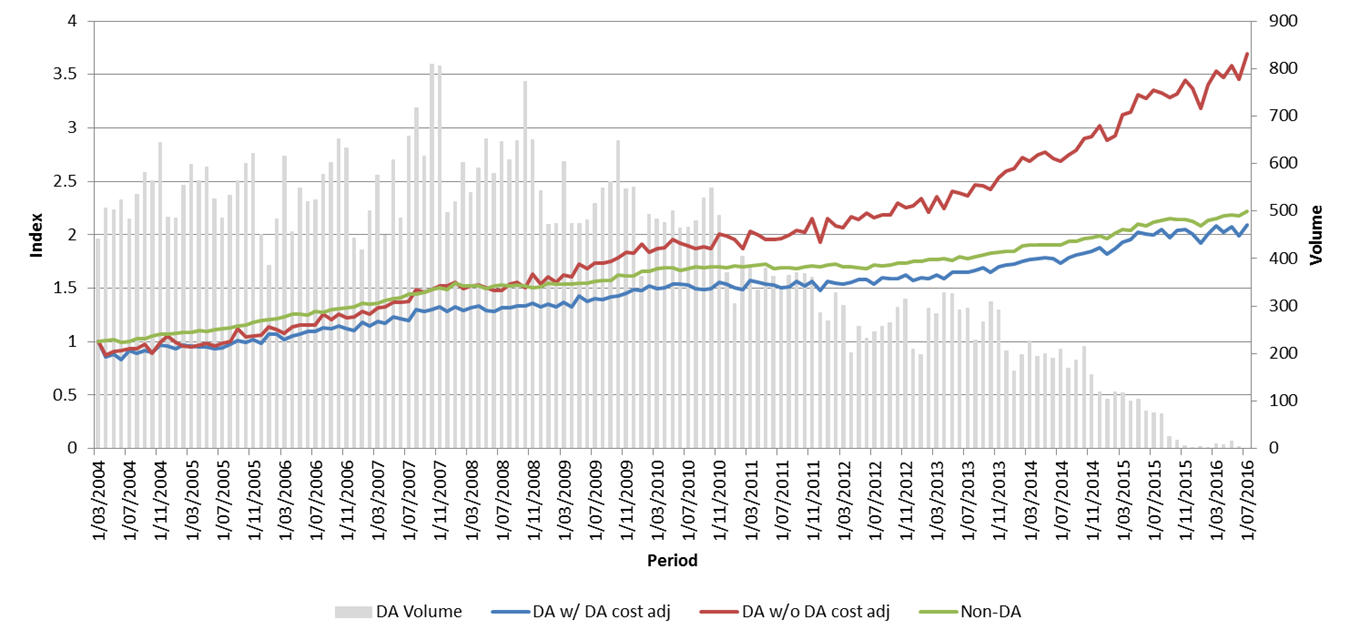
\includegraphics[width=\columnwidth]{Figures/Repeat_sales_index_post_2004_notional_purchase.png}
 \caption{Repeat Sales Index (2004-2016) - DA vs Non-DA}
 \label{fig:BMN_RS_index_post_2004}
\end{figure}

The coefficients $b_j$ on each of the dummies corresponds to the log value of the index. Therefore, we take anti-log of the regression estimates to get the raw index values. Finally, we re-base the index for the starting point - March 2004 to 1 and apply the consecutive period growth rate of the raw index to the current index value, starting from the base period - March 2004.  $\epsilon$ is the random error term in the log form with zero mean and constant variance. The notional purchase price for unimproved homes is the actual purchase price, while the notional purchase price for modified homes is the expected price at the time of DA plus the cost of development. 

%
\begin{figure}[!ht]
    \centering
  %  \textbf{Repeat Sales Index - DA and Non DA}\par\medskip
    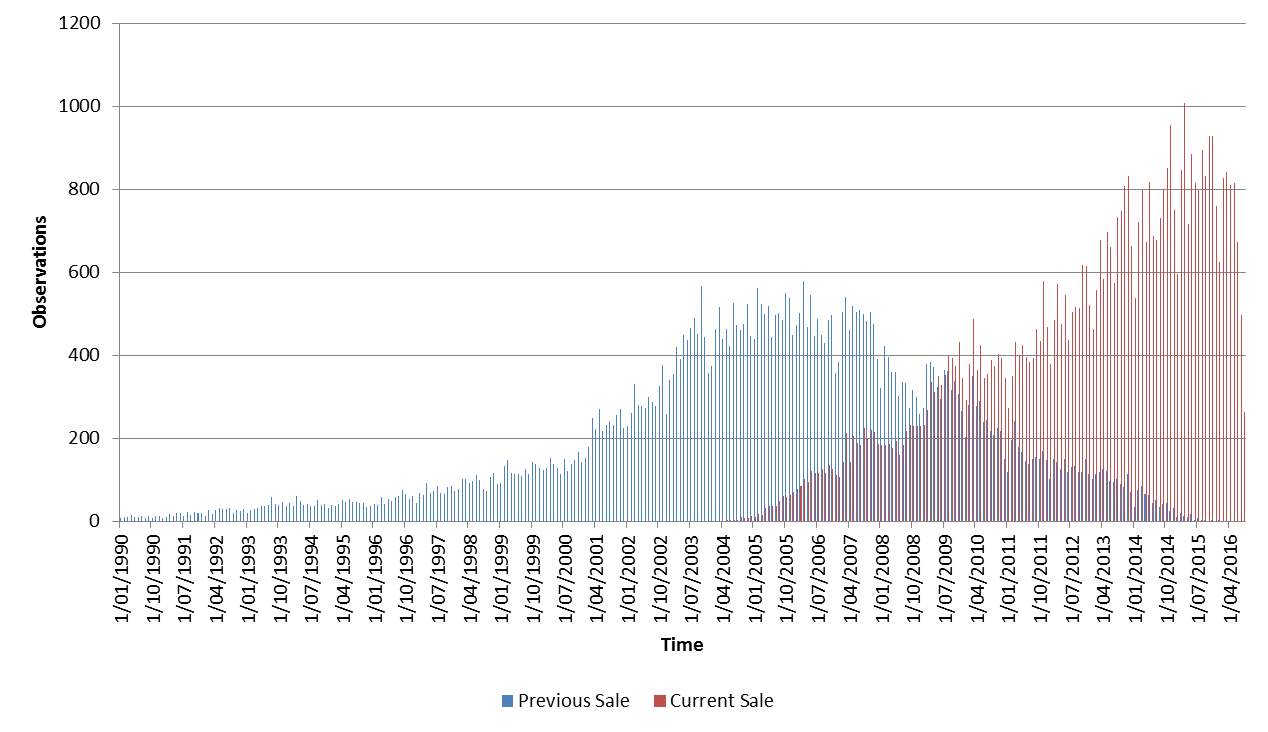
\includegraphics[width=\textwidth]{Figures/prev_cur_sale_dist.png}
    \caption{Repeat Sales Index with DA volumes}
    \label{fig:BMN}
\end{figure}
Figure \ref{fig:BMN_RS_index_post_2004} shows the repeat sales index for unimproved properties and improved properties before and after cost adjustment. The results show that, over time, the house prices for improved properties have appreciated much more than the unimproved properties. This is expected since part of the value in resale price is attributed to the home improvement. However, when we account for the improvement spending, the house price appreciation is lower than unimproved homes. For instance, if an improved and unimproved property was bought in 2004 and sold any time till 2016, the cost-adjusted house price return for improved homes would remain below unimproved homes. Therefore, over time, the returns for improved homes, on average, are lower than the unimproved homes. This is consistent with and confirms our main findings.

Since our data uses only repeat sales records, some of homes that have done improvement may not have sold yet and therefore they do not form part our data set. Hence we see that the home improvement volumes are stable from 2004 to 2010 period and then start to decline. We also see that the repeat sale index before cost adjustment is initially lower than unimproved homes. This is because there are not many observations where properties have been bought, improved and sold in the initial few years. As the time period increases, the number of observations also increase and therefore we start to see more prominent effect after the initial few years where the price appreciates at a faster rate than unimproved homes.


\subsection{Correcting Self Selection Bias}

The homes that choose to improve, on average, can be different from those that do not. There might be some random variable that is correlated with the house price return and the likelihood of improving i.e being treated, potentially introducing a self-selection bias. Therefore, in order to correct for any self-selection bias, we calculate the propensity scores for all observations using a logistic regression model and then match each improved home, i.e. from treatment sample, with unimproved homes in control sample, based on the calculated propensity scores, using the nearest neighbour method.

The logistic regression model used in calculating propensity score is given as below, \begin{equation} \label{eqn:logistic}
    DA = \alpha + \beta{P_{-1}}  + \gamma_1{Age_i} + \gamma_2{Age_i^2} + \psi{Land\_area} + \mu{K_i} + State + \epsilon_i
\end{equation}

where, $DA$ is the dummy variable coded as 1 for improved homes (treatment group) and 0 for unimproved homes (control group), $P_{-1}$ is the purchase price of the house, $Age_i$ is time between actual purchase and resale in months, $Land\_area$ is the size of the lot of land in square feet. $K_i$ is set of property attributes such as the number of bedrooms, bathrooms and car spaces and $i$ indexes the different attributes, $State$ is the state fixed effects and $\epsilon_i$ is the random error term. The set of variable that we use in the logistic regression model do not necessarily have to be same as those in the repeat sale returns model as used in main result. Rather, we use all available variables that are possibly correlated with the repeat sale returns and the likelihood of homeowners choosing to improve, to produce more reliable estimates for predicting propensity scores.

Using the estimates from the model in equation \ref{eqn:logistic}, we predict the propensity scores for all observations in both treatment and control groups. The predicted propensity scores are nothing but the expected probabilities of homeowners choosing to improve, given the set of explanatory variables used in the logistic regression. Based on the calculated propensity scores, we match each observation in treatment group of improved homes with the control group of unimproved homes using the nearest-neighbour method. We find a sample of 20,241 matched pairs of treatment and control group observations (i.e. a total of 40,482 observations). By matching the propensity scores of improved homes with unimproved homes, we are able to select homes such that the unimproved homes are equally likely of being improved, but are not. This enables us to eliminate any bias that may have, otherwise, got introduced in our sample.

The results after correcting for self-selection bias in the sample are presented in table \ref{tab:results_s0_self_select_bias}. We find that the results are robust and consistent with the main model results. Results in full model specifications -- 7 and 8, at aggregate level, show that the returns are 2.8\% and 2.7\% lower than unimproved homes, even after correcting for any potential self-selection bias. The results are also consistent across improvement types. House/Single Dwelling has the lowest return of around -13\%, followed by extension/alteration of -2.3\% and verandas/pergolas of -1.7\%. Swimming pool and carports/garages/sheds have weakly significant returns of 0.7\% and -1.4\%. Duplex has the highest return of 7.8\% as compared to unimproved homes.



\newgeometry{margin=0.5in}
% Table created by stargazer v.5.2 by Marek Hlavac, Harvard University. E-mail: hlavac at fas.harvard.edu
% Date and time: Tue, Sep 19, 2017 - 03:53:54 AM
% Requires LaTeX packages: dcolumn rotating 
\begin{sidewaystable}[!htbp] \centering 
  \caption{Self Selection Bias Correction} 
  \label{tab:results_s0_self_select_bias} 
    \resizebox{0.9\textwidth}{!}{
\begin{tabular}{@{\extracolsep{5pt}}lHH D{.}{.}{-3} D{.}{.}{-3} D{.}{.}{-3} D{.}{.}{-3} D{.}{.}{-3} D{.}{.}{-3} } 
\\[-1.8ex] 
\toprule \\[-1.8ex] 
\\[-1.8ex] & \multicolumn{8}{c}{Log(Resale Price/Purchase Price (Notional))} \\ 
\\[-1.8ex] & \multicolumn{1}{H}{(1)} & \multicolumn{1}{H}{(2)} & \multicolumn{1}{c}{(1)} & \multicolumn{1}{c}{(2)} & \multicolumn{1}{c}{(3)} & \multicolumn{1}{c}{(4)} & \multicolumn{1}{c}{(5)} & \multicolumn{1}{c}{(6)}\\ 
\midrule \\[-1.8ex] 
 DA &  &  &  &  &  &  & -0.028^{***} & -0.027^{***} \\ 
  &  &  &  &  &  &  & (0.003) & (0.003) \\ 
  %& & & & & & & & \\ 
 Carports/Garages/Sheds & -0.053^{***} & -0.022^{***} & -0.006 & -0.013^{*} & -0.013^{*} & -0.014^{*} &  &  \\ 
  & (0.008) & (0.008) & (0.008) & (0.008) & (0.008) & (0.008) &  &  \\ 
  %& & & & & & & & \\ 
 Duplex & 0.146^{***} & 0.140^{***} & 0.065^{***} & 0.066^{***} & 0.066^{***} & 0.078^{***} &  &  \\ 
  & (0.014) & (0.014) & (0.014) & (0.014) & (0.014) & (0.014) &  &  \\ 
  %& & & & & & & & \\ 
 Extension/Alteration & 0.025^{***} & 0.022^{***} & -0.023^{***} & -0.030^{***} & -0.030^{***} & -0.023^{***} &  &  \\ 
  & (0.004) & (0.004) & (0.004) & (0.004) & (0.004) & (0.004) &  &  \\ 
  %& & & & & & & & \\ 
 House/Single Dwelling & -0.045^{***} & -0.065^{***} & -0.142^{***} & -0.142^{***} & -0.142^{***} & -0.134^{***} &  &  \\ 
  & (0.007) & (0.007) & (0.007) & (0.007) & (0.007) & (0.007) &  &  \\ 
  %& & & & & & & & \\ 
 Multiple DA & 0.025^{***} & 0.005 & -0.034^{***} & -0.033^{***} & -0.033^{***} & -0.033^{***} &  &  \\ 
  & (0.007) & (0.007) & (0.007) & (0.007) & (0.007) & (0.007) &  &  \\ 
  %& & & & & & & & \\ 
 Swimming Pool & -0.034^{***} & -0.029^{***} & 0.021^{***} & 0.014^{***} & 0.014^{***} & 0.007^{*} &  &  \\ 
  & (0.004) & (0.004) & (0.004) & (0.004) & (0.004) & (0.004) &  &  \\ 
  %& & & & & & & & \\ 
 Verandahs/Pergolas & -0.055^{***} & -0.040^{***} & -0.005 & -0.015^{***} & -0.016^{***} & -0.017^{***} &  &  \\ 
  & (0.005) & (0.005) & (0.004) & (0.004) & (0.004) & (0.004) &  &  \\ 
  %& & & & & & & & \\ 
 MktReturn & 0.804^{***} & 0.794^{***} & 0.780^{***} & 0.907^{***} & 0.906^{***} & 0.905^{***} & 0.916^{***} & 0.915^{***} \\ 
  & (0.011) & (0.011) & (0.010) & (0.012) & (0.012) & (0.012) & (0.012) & (0.012) \\ 
  %& & & & & & & & \\ 
 Months between sales &  &  &  & -0.001^{***} & -0.002^{***} & -0.002^{***} & -0.002^{***} & -0.002^{***} \\ 
  &  &  &  & (0.000) & (0.000) & (0.000) & (0.000) & (0.000) \\ 
  %& & & & & & & & \\ 
 Months between sales squared &  &  &  &  & 0.000^{**} & 0.000^{**} & 0.000^{**} & 0.000^{**} \\ 
  &  &  &  &  & (0.000) & (0.000) & (0.000) & (0.000) \\ 
  %& & & & & & & & \\ 
 No. of beds (resale) &  & 0.001 & 0.032^{***} & 0.032^{***} & 0.032^{***} &  & 0.028^{***} &  \\ 
  &  & (0.002) & (0.002) & (0.002) & (0.002) &  & (0.002) &  \\ 
  %& & & & & & & & \\ 
 No. of baths (resale) &  & 0.054^{***} & 0.093^{***} & 0.092^{***} & 0.092^{***} &  & 0.084^{***} &  \\ 
  &  & (0.002) & (0.003) & (0.003) & (0.003) &  & (0.002) &  \\ 
  %& & & & & & & & \\ 
 No. of cars (resale) &  & -0.004^{***} & 0.009^{***} & 0.011^{***} & 0.011^{***} &  & 0.012^{***} &  \\ 
  &  & (0.001) & (0.001) & (0.001) & (0.001) &  & (0.001) &  \\ 
  %& & & & & & & & \\ 
 No. of beds (purchase) &  &  & -0.050^{***} & -0.050^{***} & -0.050^{***} &  & -0.043^{***} &  \\ 
  &  &  & (0.003) & (0.003) & (0.003) &  & (0.003) &  \\ 
  %& & & & & & & & \\ 
 No. of baths (purchase) &  &  & -0.094^{***} & -0.093^{***} & -0.092^{***} &  & -0.085^{***} &  \\ 
  &  &  & (0.003) & (0.003) & (0.003) &  & (0.003) &  \\ 
  %& & & & & & & & \\ 
 No. of cars (purchase) &  &  & -0.027^{***} & -0.027^{***} & -0.027^{***} &  & -0.026^{***} &  \\ 
  &  &  & (0.002) & (0.002) & (0.002) &  & (0.002) &  \\ 
  %& & & & & & & & \\ 
 Change in \# of beds &  &  &  &  &  & 0.039^{***} &  & 0.034^{***} \\ 
  &  &  &  &  &  & (0.002) &  & (0.002) \\ 
  %& & & & & & & & \\ 
 Change in \# of baths &  &  &  &  &  & 0.091^{***} &  & 0.084^{***} \\ 
  &  &  &  &  &  & (0.002) &  & (0.002) \\ 
  %& & & & & & & & \\ 
 Change in \# of cars &  &  &  &  &  & 0.016^{***} &  & 0.016^{***} \\ 
  &  &  &  &  &  & (0.001) &  & (0.001) \\ 
  %& & & & & & & & \\ 
 Constant & 0.113^{***} & -0.007 & 0.136^{***} & 0.182^{***} & 0.189^{***} & 0.097^{***} & 0.188^{***} & 0.110^{***} \\ 
  & (0.009) & (0.011) & (0.011) & (0.011) & (0.012) & (0.010) & (0.012) & (0.010) \\ 
  %& & & & & & & & \\ 
Year Fixed Effects & Yes & Yes & Yes & Yes & Yes & Yes & Yes & Yes \\ 
Location Fixed Effects & Yes & Yes & Yes & Yes & Yes & Yes & Yes & Yes  \\ 
Observations & \multicolumn{1}{H}{36,598} & \multicolumn{1}{H}{36,598} & \multicolumn{1}{c}{36,598} & \multicolumn{1}{c}{36,598} & \multicolumn{1}{c}{36,598} & \multicolumn{1}{c}{36,598} & \multicolumn{1}{c}{36,598} & \multicolumn{1}{c}{36,598} \\ 
Adjusted R$^{2}$ & \multicolumn{1}{H}{0.267} & \multicolumn{1}{H}{0.285} & \multicolumn{1}{c}{0.348} & \multicolumn{1}{c}{0.354} & \multicolumn{1}{c}{0.354} & \multicolumn{1}{c}{0.350} & \multicolumn{1}{c}{0.344} & \multicolumn{1}{c}{0.341} \\ 
F Statistic & \multicolumn{1}{H}{534.786$^{***}$} & \multicolumn{1}{H}{522.990$^{***}$} & \multicolumn{1}{c}{631.372$^{***}$} & \multicolumn{1}{c}{628.541$^{***}$} & \multicolumn{1}{c}{609.742$^{***}$} & \multicolumn{1}{c}{658.663$^{***}$} & \multicolumn{1}{c}{712.210$^{***}$} & \multicolumn{1}{c}{790.012$^{***}$} \\ 

 & \multicolumn{1}{H}{(df = 25; 36572)} & \multicolumn{1}{H}{(df = 28; 36569)} & \multicolumn{1}{c}{(df = 31; 36566)} & \multicolumn{1}{c}{(df = 32; 36565)} & \multicolumn{1}{c}{(df = 33; 36564)} & \multicolumn{1}{c}{(df = 30; 36567)} & \multicolumn{1}{c}{(df = 27; 36570)} & \multicolumn{1}{c}{(df = 24; 36573)} \\ 




%F Statistic & \multicolumn{1}{c}{534.786$^{***}$ (df = 25; 36572)} & \multicolumn{1}{c}{522.990$^{***}$ (df = 28; 36569)} & \multicolumn{1}{c}{631.372$^{***}$ (df = 31; 36566)} & \multicolumn{1}{c}{628.541$^{***}$ (df = 32; 36565)} & \multicolumn{1}{c}{609.742$^{***}$ (df = 33; 36564)} & \multicolumn{1}{c}{658.663$^{***}$ (df = 30; 36567)} & \multicolumn{1}{c}{712.210$^{***}$ (df = 27; 36570)} & \multicolumn{1}{c}{790.012$^{***}$ (df = 24; 36573)} \\ 

\bottomrule \\[-1.8ex] 
\multicolumn{9}{p{1.18\textwidth}}{Robust standard errors are reported in parentheses, Significance of variables is adjusted accordingly. *** 0.1\% significance ** 1\% significance * 5\% significance. We have a total of 40,482 (20,241 for treatment and 20,241 for control sample) possible observation with deviation accounted for by missing data.} \\ 
\end{tabular} 
}
\end{sidewaystable} 
\restoregeometry




\subsection{Sample Coverage}

In the main model results, our control sample includes properties from all the suburbs. However, different councils may have different policies in terms of disclosing development applications data. Therefore we are unsure if Cordell would have full coverage of all the development approvals received in the country. As a result, there might be some areas where homes could not be identified as improved homes even though they may have carried out improvements and inadvertently, become part of the control sample. For such properties, the value of home improvement would be implicitly accounted for in the resale price but the costs of improvement would have been ignored. This could potentially bias our main results. 

Hence to rule out any bias due to sample coverage, we use a self-selection technique to identify unbiased control group. We take all unimproved properties from suburbs that have at least one home identified with development approval. Specifically, we find a list of unique suburbs from the sample of 259,428 homes with development approvals. We don't have to use the robust sample of improved homes for identifying suburbs as this sample provides sufficient condition to rule out the councils with non-disclosure policy. 

Once we have identified the suburbs with no restriction on disclosure, we then select all properties in those suburbs with no development approvals any time between the repeat sale. This gives us our control sample of unimproved homes. Although, this method may exclude homes in suburbs where none of the properties have made any development applications at all, irrespective of the council's disclosure policy, we at least ensure that all the properties in the control sample are indeed unimproved. Using this self-selection method, we find that, out of $\sim$1.08m records of unimproved homes, only 5.5\% (60,438) records are excluded leaving us with a control sample of $\sim$1.02m unimproved homes. 

Table \ref{tab:results_s1} shows the results based a robust control sample of unimproved homes. We find that the estimates are robust and consistent with the main results. Full model specification 7 and 8 show that the returns, at aggregate level, for improved homes are 2\% and 2.4\% lower than unimproved homes. 

Also when we split by the improvement types, the results across models are generally consistent with the main results. In models 5 and 6, the return for carports is around 2.1\% and 2.6\% lower than unimproved homes. For duplex the return is 9.7\% and 10\% higher than unimproved homes. The return for extension/alteration is insignificantly different from unimproved homes. The coefficient on house single/dwelling, in both models, suggest around 10\% lower returns. The coefficient on Multiple DAs also indicate 1.2\% (weakly significant) and 1.8\% lower returns. The returns on Swimming pool is insignificant and for Verandas/Pergolas, the return is 3.8\% and 4.2\% lower than unimproved homes respectively.

\newgeometry{margin=0.5in}
% Table created by stargazer v.5.2 by Marek Hlavac, Harvard University. E-mail: hlavac at fas.harvard.edu
% Date and time: Fri, Jun 30, 2017 - 11:26:21 AM
% Requires LaTeX packages: dcolumn rotating 
\begin{sidewaystable}[!htbp] \centering 
  \caption{Sample Coverage} 
  \label{tab:results_s1} 
    \resizebox{\textwidth}{!}{
\begin{tabular}{@{\extracolsep{5pt}}lD{.}{.}{-3} D{.}{.}{-3} D{.}{.}{-3} D{.}{.}{-3} D{.}{.}{-3} D{.}{.}{-3} D{.}{.}{-3} D{.}{.}{-3} } 
\\[-1.8ex] 
\toprule \\[-1.8ex] 
\\[-1.8ex] & \multicolumn{8}{c}{Log(Resale Price/Purchase Price (Notional))} \\ 
\\[-1.8ex] & \multicolumn{1}{c}{(1)} & \multicolumn{1}{c}{(2)} & \multicolumn{1}{c}{(3)} & \multicolumn{1}{c}{(4)} & \multicolumn{1}{c}{(5)} & \multicolumn{1}{c}{(6)} & \multicolumn{1}{c}{(7)} & \multicolumn{1}{c}{(8)}\\ 
\midrule \\[-1.8ex] 
 DA &  &  &  &  &  &  & -0.020^{***} & -0.024^{***} \\ 
  &  &  &  &  &  &  & (0.002) & (0.002) \\ 
  & & & & & & & & \\ 
 Carports/Garages/Sheds & -0.091^{***} & -0.091^{***} & -0.022^{***} & -0.021^{***} & -0.021^{***} & -0.026^{***} &  &  \\ 
  & (0.007) & (0.007) & (0.007) & (0.007) & (0.007) & (0.007) &  &  \\ 
  & & & & & & & & \\ 
 Duplex & 0.179^{***} & 0.134^{***} & 0.093^{***} & 0.096^{***} & 0.097^{***} & 0.100^{***} &  &  \\ 
  & (0.012) & (0.012) & (0.013) & (0.013) & (0.013) & (0.013) &  &  \\ 
  & & & & & & & & \\ 
 Extension/Alteration & 0.026^{***} & -0.015^{***} & 0.000 & -0.000 & -0.001 & -0.002 &  &  \\ 
  & (0.003) & (0.003) & (0.004) & (0.004) & (0.004) & (0.004) &  &  \\ 
  & & & & & & & & \\ 
 House/Single Dwelling & -0.082^{***} & -0.130^{***} & -0.106^{***} & -0.102^{***} & -0.101^{***} & -0.103^{***} &  &  \\ 
  & (0.005) & (0.004) & (0.007) & (0.007) & (0.007) & (0.007) &  &  \\ 
  & & & & & & & & \\ 
 Multiple DA & 0.020^{***} & -0.021^{***} & -0.019^{***} & -0.013^{**} & -0.012^{*} & -0.018^{***} &  &  \\ 
  & (0.003) & (0.003) & (0.006) & (0.006) & (0.006) & (0.006) &  &  \\ 
  & & & & & & & & \\ 
 Swimming Pool & 0.178^{***} & 0.142^{***} & -0.002 & 0.003 & 0.003 & -0.006^{*} &  &  \\ 
  & (0.004) & (0.004) & (0.003) & (0.003) & (0.003) & (0.003) &  &  \\ 
  & & & & & & & & \\ 
 Verandahs/Pergolas & 0.008^{*} & -0.001 & -0.039^{***} & -0.037^{***} & -0.038^{***} & -0.042^{***} &  &  \\ 
  & (0.004) & (0.004) & (0.004) & (0.004) & (0.004) & (0.004) &  &  \\ 
  & & & & & & & & \\ 
 MktReturn & 0.755^{***} & 0.768^{***} & 0.808^{***} & 0.925^{***} & 0.924^{***} & 0.926^{***} & 0.925^{***} & 0.927^{***} \\ 
  & (0.002) & (0.002) & (0.003) & (0.003) & (0.003) & (0.003) & (0.003) & (0.003) \\ 
  & & & & & & & & \\ 
 Months between sales &  &  &  & -0.001^{***} & -0.002^{***} & -0.002^{***} & -0.002^{***} & -0.002^{***} \\ 
  &  &  &  & (0.000) & (0.000) & (0.000) & (0.000) & (0.000) \\ 
  & & & & & & & & \\ 
 Months between sales squared &  &  &  &  & 0.000^{***} & 0.000^{***} & 0.000^{***} & 0.000^{***} \\ 
  &  &  &  &  & (0.000) & (0.000) & (0.000) & (0.000) \\ 
  & & & & & & & & \\ 
 No. of beds (resale) &  & 0.018^{***} & 0.026^{***} & 0.027^{***} & 0.027^{***} &  & 0.026^{***} &  \\ 
  &  & (0.001) & (0.001) & (0.001) & (0.001) &  & (0.001) &  \\ 
  & & & & & & & & \\ 
 No. of baths (resale) &  & 0.050^{***} & 0.058^{***} & 0.060^{***} & 0.060^{***} &  & 0.059^{***} &  \\ 
  &  & (0.001) & (0.001) & (0.001) & (0.001) &  & (0.001) &  \\ 
  & & & & & & & & \\ 
 No. of cars (resale) &  & 0.001^{**} & 0.004^{***} & 0.006^{***} & 0.006^{***} &  & 0.006^{***} &  \\ 
  &  & (0.000) & (0.000) & (0.000) & (0.000) &  & (0.000) &  \\ 
  & & & & & & & & \\ 
 No. of beds (purchase) &  &  & -0.032^{***} & -0.033^{***} & -0.033^{***} &  & -0.032^{***} &  \\ 
  &  &  & (0.001) & (0.001) & (0.001) &  & (0.001) &  \\ 
  & & & & & & & & \\ 
 No. of baths (purchase) &  &  & -0.069^{***} & -0.069^{***} & -0.069^{***} &  & -0.069^{***} &  \\ 
  &  &  & (0.001) & (0.001) & (0.001) &  & (0.001) &  \\ 
  & & & & & & & & \\ 
 No. of cars (purchase) &  &  & -0.015^{***} & -0.016^{***} & -0.016^{***} &  & -0.016^{***} &  \\ 
  &  &  & (0.000) & (0.000) & (0.000) &  & (0.000) &  \\ 
  & & & & & & & & \\ 
 Change in \# of beds &  &  &  &  &  & 0.029^{***} &  & 0.029^{***} \\ 
  &  &  &  &  &  & (0.001) &  & (0.001) \\ 
  & & & & & & & & \\ 
 Change in \# of baths &  &  &  &  &  & 0.063^{***} &  & 0.063^{***} \\ 
  &  &  &  &  &  & (0.001) &  & (0.001) \\ 
  & & & & & & & & \\ 
 Change in \# of cars &  &  &  &  &  & 0.010^{***} &  & 0.010^{***} \\ 
  &  &  &  &  &  & (0.000) &  & (0.000) \\ 
  & & & & & & & & \\ 
 Constant & 0.103^{***} & -0.024^{**} & 0.096^{***} & 0.127^{***} & 0.142^{***} & 0.093^{***} & 0.142^{***} & 0.093^{***} \\ 
  & (0.011) & (0.012) & (0.012) & (0.012) & (0.012) & (0.012) & (0.012) & (0.012) \\ 
  & & & & & & & & \\ 
Year Fixed Effects & Yes & Yes & Yes & Yes & Yes & Yes & Yes &  \\ 
Location Fixed Effects & Yes & Yes & Yes & Yes & Yes & Yes & Yes &  \\ 
Observations & \multicolumn{1}{c}{1,085,083} & \multicolumn{1}{c}{985,860} & \multicolumn{1}{c}{508,235} & \multicolumn{1}{c}{508,235} & \multicolumn{1}{c}{508,235} & \multicolumn{1}{c}{508,235} & \multicolumn{1}{c}{508,235} & \multicolumn{1}{c}{508,235} \\ 
Adjusted R$^{2}$ & \multicolumn{1}{c}{0.128} & \multicolumn{1}{c}{0.152} & \multicolumn{1}{c}{0.285} & \multicolumn{1}{c}{0.293} & \multicolumn{1}{c}{0.293} & \multicolumn{1}{c}{0.291} & \multicolumn{1}{c}{0.293} & \multicolumn{1}{c}{0.290} \\ 
F Statistic & \multicolumn{1}{c}{5,903.084$^{***}$ (df = 27; 1085055)} & \multicolumn{1}{c}{5,888.807$^{***}$ (df = 30; 985829)} & \multicolumn{1}{c}{6,137.642$^{***}$ (df = 33; 508201)} & \multicolumn{1}{c}{6,190.773$^{***}$ (df = 34; 508200)} & \multicolumn{1}{c}{6,030.919$^{***}$ (df = 35; 508199)} & \multicolumn{1}{c}{6,517.130$^{***}$ (df = 32; 508202)} & \multicolumn{1}{c}{7,253.018$^{***}$ (df = 29; 508205)} & \multicolumn{1}{c}{7,993.324$^{***}$ (df = 26; 508208)} \\ 
\bottomrule \\[-1.8ex] 
\textit{Notes:} & \multicolumn{8}{l}{Robust standard errors in parentheses. *** 0.1\% significance ** 1\% significance * 5\% significance . 10\% significance} \\ 
\end{tabular} 
}
\end{sidewaystable} 
\restoregeometry


\subsection{Including Improved Homes Purchased Post 2004}

Since Cordell has data on development approvals available from 2004 onward, we cannot identify whether the properties were improved or not prior 2004. Therefore for the reference group - unimproved homes, we take homes purchased post 2004 only. For treatment group however, we take properties purchased post 1990. Also since these are classified as improved homes, there will be relatively a smaller portion of properties that may have carried out additional improvement prior 2004. Any value attributed to the improvement prior 2004 will be implicit in the resale price but the improvement cost prior 2004, would not have been accounted for and therefore the total cost of development for improved homes would only be underestimated for such properties, which, in aggregate, makes the estimates even more negative. Hence, it does not affect our main analysis adversely. Also, in the interest of having a reasonable sample size, we include all the homes  in the main analysis.

Nonetheless, as part of robustness, we test the results to ensure that the estimates are consistent and stable after excluding all homes purchased prior 2004 for improved homes as well. To make the model even more robust, we also exclude the properties from the control group of unimproved homes that may induce sample coverage bias. Table \ref{tab:result_s1_prev2004} presents the results with all homes purchased after 2004 included in the analysis. We find that the results are all consistent with the main results. 

In model 7 and 8, the returns for improved homes is 1.8\% and 2.2\% lower than unimproved homes respectively. When we look at by different improvement types, the returns, according to models 1 through 6 are generally consistent with the main results. In models 5 and 6, the coefficient for carports/garages/sheds is -1.9\% and -2.4\%. The returns for duplex is around 9\% higher than unimproved homes. For extension/alterations, the returns are insignificant. For House/Single Dwelling the returns are around 10\% lower than unimproved homes. In case of Multiple DAs and swimming pools, the returns are insignificantly different from unimproved homes (model 5) and weakly significant at -1.4\% and -0.8\% (model 6) respectively. For Verandas/pergolas, the returns are around 3\% lower than unimproved homes.

\newgeometry{margin=0.5in}
% Table created by stargazer v.5.2 by Marek Hlavac, Harvard University. E-mail: hlavac at fas.harvard.edu
% Date and time: Fri, Jun 30, 2017 - 11:11:20 AM
% Requires LaTeX packages: dcolumn rotating 
\begin{sidewaystable}[!htbp] \centering 
  \caption{Including Improved Homes Purchased Post 2004} 
  \label{tab:result_s1_prev2004} 
  \resizebox{\textwidth}{!}{
\begin{threeparttable}

\begin{tabular}{@{\extracolsep{5pt}}lD{.}{.}{-3} D{.}{.}{-3} D{.}{.}{-3} D{.}{.}{-3} D{.}{.}{-3} D{.}{.}{-3} } 
\\[-1.8ex] 
\toprule \\[-1.8ex] 
\\[-1.8ex] & \multicolumn{6}{c}{Log(Resale Price/Purchase Price (Notional))} \\ 
\\[-1.8ex] & \multicolumn{1}{c}{(1)} & \multicolumn{1}{c}{(2)} & \multicolumn{1}{c}{(3)} & \multicolumn{1}{c}{(4)} & \multicolumn{1}{c}{(5)} & \multicolumn{1}{c}{(6)}\\ 
\midrule \\[-1.8ex] 
 DA &  &  &  &  & -0.018^{***} & -0.022^{***} \\ 
  &  &  &  &  & (0.002) & (0.002) \\ 
  %& & & & & & \\ 
 Carports/Garages/Sheds & -0.020^{***} & -0.020^{***} & -0.019^{***} & -0.024^{***} &  &  \\ 
  & (0.007) & (0.007) & (0.007) & (0.007) &  &  \\ 
  %& & & & & & \\ 
 Duplex & 0.090^{***} & 0.091^{***} & 0.093^{***} & 0.095^{***} &  &  \\ 
  & (0.014) & (0.014) & (0.014) & (0.014) &  &  \\ 
  %& & & & & & \\ 
 Extension/Alteration & 0.008^{**} & 0.006 & 0.005 & 0.004 &  &  \\ 
  & (0.004) & (0.004) & (0.004) & (0.004) &  &  \\ 
  %& & & & & & \\ 
 House/Single Dwelling & -0.106^{***} & -0.102^{***} & -0.101^{***} & -0.103^{***} &  &  \\ 
  & (0.007) & (0.007) & (0.007) & (0.007) &  &  \\ 
  %& & & & & & \\ 
 Multiple DA & -0.013^{*} & -0.008 & -0.008 & -0.014^{**} &  &  \\ 
  & (0.007) & (0.007) & (0.007) & (0.007) &  &  \\ 
  %& & & & & & \\ 
 Swimming Pool & -0.003 & 0.001 & 0.002 & -0.008^{**} &  &  \\ 
  & (0.004) & (0.004) & (0.004) & (0.004) &  &  \\ 
  %& & & & & & \\ 
 Verandahs/Pergolas & -0.032^{***} & -0.031^{***} & -0.032^{***} & -0.036^{***} &  &  \\ 
  & (0.004) & (0.004) & (0.004) & (0.004) &  &  \\ 
  %& & & & & & \\ 
 MktReturn & 0.808^{***} & 0.926^{***} & 0.926^{***} & 0.927^{***} & 0.926^{***} & 0.928^{***} \\ 
  & (0.003) & (0.003) & (0.003) & (0.003) & (0.003) & (0.003) \\ 
  %& & & & & & \\ 
 Months between sales &  & -0.001^{***} & -0.002^{***} & -0.002^{***} & -0.002^{***} & -0.002^{***} \\ 
  &  & (0.000) & (0.000) & (0.000) & (0.000) & (0.000) \\ 
  %& & & & & & \\ 
 Months between sales squared &  &  & 0.000^{***} & 0.000^{***} & 0.000^{***} & 0.000^{***} \\ 
  &  &  & (0.000) & (0.000) & (0.000) & (0.000) \\ 
  %& & & & & & \\ 
 No. of beds (resale) & 0.026^{***} & 0.027^{***} & 0.027^{***} &  & 0.026^{***} &  \\ 
  & (0.001) & (0.001) & (0.001) &  & (0.001) &  \\ 
  %& & & & & & \\ 
 No. of baths (resale) & 0.058^{***} & 0.059^{***} & 0.059^{***} &  & 0.059^{***} &  \\ 
  & (0.001) & (0.001) & (0.001) &  & (0.001) &  \\ 
  %& & & & & & \\ 
 No. of cars (resale) & 0.004^{***} & 0.006^{***} & 0.006^{***} &  & 0.006^{***} &  \\ 
  & (0.000) & (0.000) & (0.000) &  & (0.000) &  \\ 
  %& & & & & & \\ 
 No. of beds (purchase) & -0.032^{***} & -0.033^{***} & -0.033^{***} &  & -0.032^{***} &  \\ 
  & (0.001) & (0.001) & (0.001) &  & (0.001) &  \\ 
  %& & & & & & \\ 
 No. of baths (purchase) & -0.069^{***} & -0.069^{***} & -0.069^{***} &  & -0.068^{***} &  \\ 
  & (0.001) & (0.001) & (0.001) &  & (0.001) &  \\ 
  %& & & & & & \\ 
 No. of cars (purchase) & -0.015^{***} & -0.016^{***} & -0.016^{***} &  & -0.016^{***} &  \\ 
  & (0.000) & (0.000) & (0.000) &  & (0.000) &  \\ 
  %& & & & & & \\ 
 Change in \# of beds &  &  &  & 0.029^{***} &  & 0.029^{***} \\ 
  &  &  &  & (0.001) &  & (0.001) \\ 
  %& & & & & & \\ 
 Change in \# of baths &  &  &  & 0.063^{***} &  & 0.063^{***} \\ 
  &  &  &  & (0.001) &  & (0.001) \\ 
  %& & & & & & \\ 
 Change in \# of cars &  &  &  & 0.010^{***} &  & 0.010^{***} \\ 
  &  &  &  & (0.000) &  & (0.000) \\ 
  %& & & & & & \\ 
 Constant & 0.086^{***} & 0.111^{***} & 0.127^{***} & 0.076^{***} & 0.127^{***} & 0.076^{***} \\ 
  & (0.002) & (0.002) & (0.003) & (0.002) & (0.003) & (0.002) \\ 
  %& & & & & & \\ 
Year Fixed Effects & Yes & Yes & Yes & Yes & Yes & Yes \\ 
Location Fixed Effects & Yes & Yes & Yes & Yes & Yes & Yes \\ 
Observations & \multicolumn{1}{c}{504,893} & \multicolumn{1}{c}{504,893} & \multicolumn{1}{c}{504,893} & \multicolumn{1}{c}{504,893} & \multicolumn{1}{c}{504,893} & \multicolumn{1}{c}{504,893} \\ 
Adjusted R$^{2}$ & \multicolumn{1}{c}{0.284} & \multicolumn{1}{c}{0.292} & \multicolumn{1}{c}{0.292} & \multicolumn{1}{c}{0.290} & \multicolumn{1}{c}{0.292} & \multicolumn{1}{c}{0.289} \\ 
F Statistic & \multicolumn{1}{c}{6,452.740$^{***}$ (df = 31; 504861)} & \multicolumn{1}{c}{6,498.731$^{***}$ (df = 32; 504860)} & \multicolumn{1}{c}{6,320.072$^{***}$ (df = 33; 504859)} & \multicolumn{1}{c}{6,867.966$^{***}$ (df = 30; 504862)} & \multicolumn{1}{c}{7,699.735$^{***}$ (df = 27; 504865)} & \multicolumn{1}{c}{8,557.664$^{***}$ (df = 24; 504868)} \\ 



\bottomrule \\[-1.8ex] 

\end{tabular} 

\begin{tablenotes}[para,flushleft]
  \LARGE
      Notes: Robust standard errors are reported in parentheses, Significance of variables is adjusted accordingly. *** 0.1\% significance ** 1\% significance * 5\% significance. We have a total of 1,064,462 (36,894 for treatment and 1,027,568 for control sample) possible observation with deviation accounted for by missing data.
\end{tablenotes}    



\end{threeparttable}
}
\end{sidewaystable} 
\restoregeometry


\section{Conclusion}

This paper explores and compares an important economic decision faced by homeowners on the returns of improved homes in relation to the unimproved homes. Using a combined data set of house prices and development applications, we test if the returns for improved home is better than unimproved homes. We find that the returns for improved homes, in aggregate, is lower than unimproved homes by around 2.4\%. If we split by improvement types, we find that the highest loss is in building a new house/single dwelling with around 10\% lower returns than unimproved homes. This is mainly attributed to the opportunity cost of lost building value. Carports/Garages/Sheds has around 2.5\% lower returns while verandas/pergolas has around 4.2\% lower return. The return on extension/alteration and swimming pool is not significantly different from unimproved homes. In contrast, the returns for Duplex are higher than the unimproved homes by around 10\% and this is due to the double equity generated from the land-split.

In a further analysis, we examine and compare the returns for two types of investors and owner occupiers who buy for their own personal living. Type I investors are classified as speculators/flippers with buy-improve-sell strategy who buy and sell within two years and type II are those homeowners with improve-and-sell strategy who buy and sell in more than 2 years but invest at some later point to improve their homes and then sell within two years of home improvement. We used an interaction variable between investor and DA dummies and at aggregate level, we find that the returns for improved homes for type I investors are higher than unimproved homes by around 0.4\%. The positive change in the main result is much more prominent in the extension/alteration - around 5.4\% higher than the unimproved homes compared to the insignificant returns in the main results. This explains why typically speculators/flippers mainly would perform extension/alterations as part of their investment strategy. The returns on carports and verandas/pergolas has also improved from negative to being insignificant. 

In contrast, for type II investors, in aggregate, we find that the returns for improved homes are lower than the unimproved homes by around 1.2\%. When we condition on data, where time between improvement and resale is less than 2 years and split by improvement type, we see that the returns across improvement types have reduced as compared to the main result. This is because the reference category (unimproved homes) in both the analysis - investor type I and investor type II, is conditioned by the time between purchase and resale as less than 2 years. Therefore, since, the return for speculator group in the reference category, on average, is higher than the non-speculator group, the returns on improved homes are even lower. The return on Duplex is reduced from around 10\% to 5.5\%. The return on Extension/alteration has gone from being insignificant to negative 3\%. The returns on house is reduced further to around 22\%. Verandas/Pergolas also reduced to 7\% lower returns. 

So overall this suggests, that homeowners with speculative motive who buy and sell the property in less than two years have higher returns from home improvements; whereas homeowners who owned the property for more than two years but sell the property in less than two years from carrying out home improvement perform worse. This further suggests that the time between sales is the instrumental variable that enables identification of homeowners with investment motive, however quick turnaround time may not necessarily imply higher return. And homeowners who have a financial motive make higher returns while those who are non-speculators with a consumption motive have lower returns. 

The returns on home improvement can be affected by the four main factors - (a) the high cost of home improvement - as the cost of improvement rises, the return on home improvement will decrease. However, since speculators/flippers also incur the same cost of improvement, and yet are able to make positive returns, particularly on the extension/alterations, suggests that at given levels of improvement cost, there are still positive returns to be made and therefore the lower returns cannot be completely attributed the high cost of improvement. (b) Depreciation - Since the homeowners with consumption motive consume the housing services, there would be additional costs in terms of the lost building value in the form of physical deterioration. However, the depreciation effect is already controlled for in the model and therefore the lower returns of 2.4\% estimated in the model should be over and above the depreciation costs. (c) Absolute profits from house price appreciation - Homeowners enjoy profits, when they resell their home, from house price appreciation which is mainly attributed to the growth in the value of land. As a result, at the time of resale, homeowners may be more psychologically willing to settle for reduced profits without realizing that this may result in negative returns on home improvement. (d) Overcapitalizing - the homeowners with consumption motive are operating in the long run and therefore their decision and choices, as opposed to homeowners with speculative motive, are guided by non-economic reasons. For example, while a speculator would probably add a smaller bedroom or bathroom (as there are diminishing returns to housing), the homeowners with consumption motive would rather choose to build the size of the bedrooms or bathrooms based on their personal needs and affordability and hence end up over spending on the improvements. This explains why speculators are able to make financial gains while the homeowners with a consumption motive, on the other hand, rather enjoy the non-monetary benefits. The relative loss that we estimate in our models is probably the price of such benefits. %In a simplistic sense, our paper models and examines the returns on two basic options - 'improve' or 'do-nothing'. However, homeowners may also face another option and that is - 'moving' to a new desired home. Comparing the returns between 'improving' or 'moving' could be an avenue for future research.



\bibliographystyle{aer}
\bibliography{sample}


\appendix


%\setcounter{table}{0}
\renewcommand{\thetable}{A\arabic{table}}
%\renewcommand{\thetable}{\Alph{section}\arabic{table}}

\newgeometry{margin=0.5in}

% Table created by stargazer v.5.2 by Marek Hlavac, Harvard University. E-mail: hlavac at fas.harvard.edu
% Date and time: Tue, Aug 29, 2017 - 11:13:06 AM
% Requires LaTeX packages: dcolumn rotating 
\begin{sidewaystable}[!htbp] \centering 
  \caption{Main Result Robustness - Full DA Sample} 
  \label{Main_result_201k_sample} 
  \resizebox{\textwidth}{!}{
\begin{threeparttable}

\begin{tabular}{@{\extracolsep{5pt}}lD{.}{.}{-3} D{.}{.}{-3} D{.}{.}{-3} D{.}{.}{-3} D{.}{.}{-3} D{.}{.}{-3} } 
\\[-1.8ex]\hline 
\hline \\[-1.8ex] 
\\[-1.8ex] & \multicolumn{6}{c}{Log(Resale Price/Purchase Price (Notional))} \\ 
\\[-1.8ex] & \multicolumn{1}{c}{(1)} & \multicolumn{1}{c}{(2)} & \multicolumn{1}{c}{(3)} & \multicolumn{1}{c}{(4)} & \multicolumn{1}{c}{(5)} & \multicolumn{1}{c}{(6)}\\ 
\hline \\[-1.8ex] 
 DA &  &  &  &  & -0.051^{***} & -0.054^{***} \\ 
  &  &  &  &  & (0.002) & (0.002) \\ 
  & & & & & & \\ 
 Carports/Garages/Sheds & -0.041^{***} & -0.042^{***} & -0.043^{***} & -0.045^{***} &  &  \\ 
  & (0.004) & (0.004) & (0.004) & (0.004) &  &  \\ 
  & & & & & & \\ 
 Duplex & 0.074^{***} & 0.077^{***} & 0.078^{***} & 0.082^{***} &  &  \\ 
  & (0.013) & (0.013) & (0.013) & (0.013) &  &  \\ 
  & & & & & & \\ 
 Extension/Alteration & -0.026^{***} & -0.027^{***} & -0.028^{***} & -0.029^{***} &  &  \\ 
  & (0.003) & (0.003) & (0.003) & (0.003) &  &  \\ 
  & & & & & & \\ 
 House/Single Dwelling & -0.173^{***} & -0.169^{***} & -0.169^{***} & -0.170^{***} &  &  \\ 
  & (0.005) & (0.005) & (0.005) & (0.005) &  &  \\ 
  & & & & & & \\ 
 Multiple DA & -0.071^{***} & -0.067^{***} & -0.067^{***} & -0.071^{***} &  &  \\ 
  & (0.005) & (0.005) & (0.005) & (0.005) &  &  \\ 
  & & & & & & \\ 
 Swimming Pool & -0.017^{***} & -0.015^{***} & -0.015^{***} & -0.023^{***} &  &  \\ 
  & (0.003) & (0.003) & (0.003) & (0.003) &  &  \\ 
  & & & & & & \\ 
 Verandas/Pergolas & -0.042^{***} & -0.040^{***} & -0.041^{***} & -0.045^{***} &  &  \\ 
  & (0.004) & (0.004) & (0.004) & (0.004) &  &  \\ 
  & & & & & & \\ 
 MktReturn & 0.806^{***} & 0.923^{***} & 0.923^{***} & 0.925^{***} & 0.924^{***} & 0.926^{***} \\ 
  & (0.003) & (0.003) & (0.003) & (0.003) & (0.003) & (0.003) \\ 
  & & & & & & \\ 
 Age &  & -0.001^{***} & -0.002^{***} & -0.002^{***} & -0.002^{***} & -0.002^{***} \\ 
  &  & (0.000) & (0.000) & (0.000) & (0.000) & (0.000) \\ 
  & & & & & & \\ 
 Age squared &  &  & 0.000^{***} & 0.000^{***} & 0.000^{***} & 0.000^{***} \\ 
  &  &  & (0.000) & (0.000) & (0.000) & (0.000) \\ 
  & & & & & & \\ 
 No. of beds (resale) & 0.028^{***} & 0.028^{***} & 0.028^{***} &  & 0.028^{***} &  \\ 
  & (0.001) & (0.001) & (0.001) &  & (0.001) &  \\ 
  & & & & & & \\ 
 No. of baths (resale) & 0.062^{***} & 0.063^{***} & 0.063^{***} &  & 0.062^{***} &  \\ 
  & (0.001) & (0.001) & (0.001) &  & (0.001) &  \\ 
  & & & & & & \\ 
 No. of cars (resale) & 0.004^{***} & 0.006^{***} & 0.006^{***} &  & 0.006^{***} &  \\ 
  & (0.000) & (0.000) & (0.000) &  & (0.000) &  \\ 
  & & & & & & \\ 
 No. of beds (purchase) & -0.033^{***} & -0.034^{***} & -0.034^{***} &  & -0.033^{***} &  \\ 
  & (0.001) & (0.001) & (0.001) &  & (0.001) &  \\ 
  & & & & & & \\ 
 No. of baths (purchase) & -0.071^{***} & -0.071^{***} & -0.071^{***} &  & -0.070^{***} &  \\ 
  & (0.001) & (0.001) & (0.001) &  & (0.001) &  \\ 
  & & & & & & \\ 
 No. of cars (purchase) & -0.016^{***} & -0.016^{***} & -0.016^{***} &  & -0.016^{***} &  \\ 
  & (0.000) & (0.000) & (0.000) &  & (0.000) &  \\ 
  & & & & & & \\ 
 Change in \# of beds &  &  &  & 0.030^{***} &  & 0.030^{***} \\ 
  &  &  &  & (0.001) &  & (0.001) \\ 
  & & & & & & \\ 
 Change in \# of baths &  &  &  & 0.066^{***} &  & 0.065^{***} \\ 
  &  &  &  & (0.001) &  & (0.001) \\ 
  & & & & & & \\ 
 Change in \# of cars &  &  &  & 0.010^{***} &  & 0.010^{***} \\ 
  &  &  &  & (0.000) &  & (0.000) \\ 
  & & & & & & \\ 
 Constant & 0.084^{***} & 0.109^{***} & 0.122^{***} & 0.075^{***} & 0.123^{***} & 0.076^{***} \\ 
  & (0.002) & (0.002) & (0.003) & (0.002) & (0.003) & (0.002) \\ 
  & & & & & & \\ 
Year Fixed Effects & Yes & Yes & Yes & Yes & Yes & Yes \\ 
Location Fixed Effects & Yes & Yes & Yes & Yes & Yes & Yes \\ 
Observations & \multicolumn{1}{c}{529,063} & \multicolumn{1}{c}{529,063} & \multicolumn{1}{c}{529,063} & \multicolumn{1}{c}{529,063} & \multicolumn{1}{c}{529,063} & \multicolumn{1}{c}{529,063} \\ 
Adjusted R$^{2}$ & \multicolumn{1}{c}{0.281} & \multicolumn{1}{c}{0.289} & \multicolumn{1}{c}{0.289} & \multicolumn{1}{c}{0.287} & \multicolumn{1}{c}{0.287} & \multicolumn{1}{c}{0.285} \\ 
F Statistic & \multicolumn{1}{c}{6,677.688$^{***}$ (df = 31; 529031)} & \multicolumn{1}{c}{6,718.845$^{***}$ (df = 32; 529030)} & \multicolumn{1}{c}{6,529.027$^{***}$ (df = 33; 529029)} & \multicolumn{1}{c}{7,108.311$^{***}$ (df = 30; 529032)} & \multicolumn{1}{c}{7,900.302$^{***}$ (df = 27; 529035)} & \multicolumn{1}{c}{8,797.499$^{***}$ (df = 24; 529038)} \\ 



\bottomrule \\[-1.8ex] 

\end{tabular} 

\begin{tablenotes}[para,flushleft]
  \LARGE
      Notes: Robust standard errors are reported in parentheses, Significance of variables is adjusted accordingly. *** 0.1\% significance ** 1\% significance * 5\% significance. We have a total of 1,263,893 (200,207 for treatment and 1,063,686 for control sample) possible observation with deviation accounted for by missing data.
\end{tablenotes}    



\end{threeparttable}
}
\end{sidewaystable} 
\restoregeometry 


\newgeometry{margin=0.5in}
% Table created by stargazer v.5.2 by Marek Hlavac, Harvard University. E-mail: hlavac at fas.harvard.edu
% Date and time: Wed, Jun 14, 2017 - 04:52:42 AM
% Requires LaTeX packages: dcolumn rotating 
\begin{sidewaystable}[!htbp] \centering 
  \caption{Fixed Effects Model Results - SSD Region level} 
  \label{tab:results_ssd}
    \resizebox{\textwidth}{!}{
\begin{threeparttable}

\begin{tabular}{@{\extracolsep{5pt}}lD{.}{.}{-3} D{.}{.}{-3} D{.}{.}{-3} D{.}{.}{-3} D{.}{.}{-3} D{.}{.}{-3} D{.}{.}{-3} D{.}{.}{-3} } 
\\[-1.8ex] 
\toprule \\[-1.8ex] 
\\[-1.8ex] & \multicolumn{8}{c}{Log(Resale Price/Purchase Price (Notional))} \\ 
\\[-1.8ex] & \multicolumn{1}{c}{(1)} & \multicolumn{1}{c}{(2)} & \multicolumn{1}{c}{(3)} & \multicolumn{1}{c}{(4)} & \multicolumn{1}{c}{(5)} & \multicolumn{1}{c}{(6)} & \multicolumn{1}{c}{(7)} & \multicolumn{1}{c}{(8)}\\ 
\midrule \\[-1.8ex] 
 DA &  &  &  &  &  &  & -0.019^{***} & -0.024^{***} \\ 
  &  &  &  &  &  &  & (0.002) & (0.002) \\ 
  %& & & & & & & & \\ 
 Carports/Garages/Sheds & -0.070^{***} & -0.074^{***} & -0.002 & -0.001 & -0.000 & -0.005 &  &  \\ 
  & (0.007) & (0.007) & (0.007) & (0.007) & (0.006) & (0.007) &  &  \\ 
  %& & & & & & & & \\ 
 Duplex & 0.160^{***} & 0.114^{***} & 0.084^{***} & 0.094^{***} & 0.096^{***} & 0.096^{***} &  &  \\ 
  & (0.012) & (0.012) & (0.013) & (0.013) & (0.013) & (0.013) &  &  \\ 
  %& & & & & & & & \\ 
 Extension/Alteration & 0.029^{***} & -0.009^{***} & -0.009^{***} & -0.010^{***} & -0.010^{***} & -0.012^{***} &  &  \\ 
  & (0.003) & (0.003) & (0.004) & (0.004) & (0.004) & (0.004) &  &  \\ 
  %& & & & & & & & \\ 
 House/Single Dwelling & -0.080^{***} & -0.125^{***} & -0.117^{***} & -0.110^{***} & -0.109^{***} & -0.111^{***} &  &  \\ 
  & (0.005) & (0.005) & (0.007) & (0.007) & (0.007) & (0.007) &  &  \\ 
  %& & & & & & & & \\ 
 Multiple DA & 0.034^{***} & -0.005 & -0.023^{***} & -0.015^{**} & -0.015^{**} & -0.021^{***} &  &  \\ 
  & (0.003) & (0.003) & (0.006) & (0.006) & (0.006) & (0.006) &  &  \\ 
  %& & & & & & & & \\ 
 Swimming Pool & 0.189^{***} & 0.156^{***} & 0.002 & 0.007^{**} & 0.007^{**} & -0.002 &  &  \\ 
  & (0.004) & (0.004) & (0.003) & (0.003) & (0.003) & (0.003) &  &  \\ 
  %& & & & & & & & \\ 
 Verandahs/Pergolas & 0.024^{***} & 0.015^{***} & -0.028^{***} & -0.026^{***} & -0.027^{***} & -0.031^{***} &  &  \\ 
  & (0.004) & (0.004) & (0.003) & (0.003) & (0.003) & (0.003) &  &  \\ 
  %& & & & & & & & \\ 
 MktReturn & 0.766^{***} & 0.775^{***} & 0.809^{***} & 0.955^{***} & 0.954^{***} & 0.954^{***} & 0.955^{***} & 0.955^{***} \\ 
  & (0.002) & (0.003) & (0.003) & (0.003) & (0.003) & (0.003) & (0.003) & (0.003) \\ 
  %& & & & & & & & \\ 
 Months between sales &  &  &  & -0.001^{***} & -0.002^{***} & -0.002^{***} & -0.002^{***} & -0.002^{***} \\ 
  &  &  &  & (0.000) & (0.000) & (0.000) & (0.000) & (0.000) \\ 
  %& & & & & & & & \\ 
 Months between sales squared &  &  &  &  & 0.000^{***} & 0.000^{***} & 0.000^{***} & 0.000^{***} \\ 
  &  &  &  &  & (0.000) & (0.000) & (0.000) & (0.000) \\ 
  %& & & & & & & & \\ 
 No. of beds (resale) &  & 0.016^{***} & 0.025^{***} & 0.026^{***} & 0.026^{***} &  & 0.025^{***} &  \\ 
  &  & (0.001) & (0.001) & (0.001) & (0.001) &  & (0.001) &  \\ 
  %& & & & & & & & \\ 
 No. of baths (resale) &  & 0.054^{***} & 0.051^{***} & 0.052^{***} & 0.052^{***} &  & 0.051^{***} &  \\ 
  &  & (0.001) & (0.001) & (0.001) & (0.001) &  & (0.001) &  \\ 
  %& & & & & & & & \\ 
 No. of cars (resale) &  & 0.001^{***} & 0.006^{***} & 0.008^{***} & 0.008^{***} &  & 0.008^{***} &  \\ 
  &  & (0.000) & (0.000) & (0.000) & (0.000) &  & (0.000) &  \\ 
  %& & & & & & & & \\ 
 No. of beds (purchase) &  &  & -0.031^{***} & -0.031^{***} & -0.031^{***} &  & -0.031^{***} &  \\ 
  &  &  & (0.001) & (0.001) & (0.001) &  & (0.001) &  \\ 
  %& & & & & & & & \\ 
 No. of baths (purchase) &  &  & -0.070^{***} & -0.070^{***} & -0.070^{***} &  & -0.069^{***} &  \\ 
  &  &  & (0.001) & (0.001) & (0.001) &  & (0.001) &  \\ 
  %& & & & & & & & \\ 
 No. of cars (purchase) &  &  & -0.013^{***} & -0.014^{***} & -0.014^{***} &  & -0.014^{***} &  \\ 
  &  &  & (0.000) & (0.000) & (0.000) &  & (0.000) &  \\ 
  %& & & & & & & & \\ 
 Change in \# of beds &  &  &  &  &  & 0.028^{***} &  & 0.027^{***} \\ 
  &  &  &  &  &  & (0.001) &  & (0.001) \\ 
  %& & & & & & & & \\ 
 Change in \# of baths &  &  &  &  &  & 0.060^{***} &  & 0.059^{***} \\ 
  &  &  &  &  &  & (0.001) &  & (0.001) \\ 
  %& & & & & & & & \\ 
 Change in \# of cars &  &  &  &  &  & 0.010^{***} &  & 0.010^{***} \\ 
  &  &  &  &  &  & (0.000) &  & (0.000) \\ 
  %& & & & & & & & \\ 
 Constant & 0.148^{***} & 0.023^{***} & 0.160^{***} & 0.179^{***} & 0.194^{***} & 0.143^{***} & 0.193^{***} & 0.144^{***} \\ 
  & (0.004) & (0.006) & (0.006) & (0.006) & (0.006) & (0.006) & (0.006) & (0.006) \\ 
  %& & & & & & & & \\ 
Year Fixed Effects & Yes & Yes & Yes & Yes & Yes & Yes & Yes & Yes \\ 
Location Fixed Effects & Yes & Yes & Yes & Yes & Yes & Yes & Yes & Yes \\ 
Observations & \multicolumn{1}{c}{1,119,293} & \multicolumn{1}{c}{1,012,436} & \multicolumn{1}{c}{517,011} & \multicolumn{1}{c}{517,011} & \multicolumn{1}{c}{517,011} & \multicolumn{1}{c}{517,011} & \multicolumn{1}{c}{517,011} & \multicolumn{1}{c}{517,011} \\ 
Adjusted R$^{2}$ & \multicolumn{1}{c}{0.140} & \multicolumn{1}{c}{0.165} & \multicolumn{1}{c}{0.302} & \multicolumn{1}{c}{0.311} & \multicolumn{1}{c}{0.312} & \multicolumn{1}{c}{0.309} & \multicolumn{1}{c}{0.311} & \multicolumn{1}{c}{0.308} \\ 
%F Statistic & \multicolumn{1}{c}{887.768$^{***}$ (df = 206; 1119086)} & \multicolumn{1}{c}{955.373$^{***}$ (df = 209; 1012226)} & \multicolumn{1}{c}{1,057.003$^{***}$ (df = 212; 516798)} & \multicolumn{1}{c}{1,098.319$^{***}$ (df = 213; 516797)} & \multicolumn{1}{c}{1,096.034$^{***}$ (df = 214; 516796)} & \multicolumn{1}{c}{1,095.434$^{***}$ (df = 211; 516799)} & \multicolumn{1}{c}{1,123.717$^{***}$ (df = 208; 516802)} & \multicolumn{1}{c}{1,123.728$^{***}$ (df = 205; 516805)} \\ 

F Statistic & \multicolumn{1}{c}{887.768$^{***}$} & \multicolumn{1}{c}{955.373$^{***}$} & \multicolumn{1}{c}{1,057.003$^{***}$} & \multicolumn{1}{c}{1,098.319$^{***}$} & \multicolumn{1}{c}{1,096.034$^{***}$} & \multicolumn{1}{c}{1,095.434$^{***}$} & \multicolumn{1}{c}{1,123.717$^{***}$} & \multicolumn{1}{c}{1,123.728$^{***}$} \\ 

& \multicolumn{1}{c}{(df = 206; 1119086)} & \multicolumn{1}{c}{(df = 209; 1012226)} & \multicolumn{1}{c}{(df = 212; 516798)} & \multicolumn{1}{c}{(df = 213; 516797)} & \multicolumn{1}{c}{(df = 214; 516796)} & \multicolumn{1}{c}{(df = 211; 516799)} & \multicolumn{1}{c}{(df = 208; 516802)} & \multicolumn{1}{c}{(df = 205; 516805)} \\ 

\bottomrule \\[-1.8ex] 
%\textit{Notes:} & \multicolumn{8}{l}{Robust standard errors in parentheses. *** 0.1\% significance ** 1\% significance * 5\% significance . 10\% significance} \\

\end{tabular}%

\begin{tablenotes}[para,flushleft]
  \LARGE
      Notes: Robust standard errors are reported in parentheses, Significance of variables is adjusted accordingly. *** 0.1\% significance ** 1\% significance * 5\% significance. We have a total of 1,119,419 (55,733 for treatment and 1,063,686 for control sample) possible observation with deviation accounted for by missing data.
\end{tablenotes}    



\end{threeparttable}
}
\end{sidewaystable} 
\restoregeometry 


\clearpage

%\section{Appendix B}

\begin{figure}[!h]
    \centering
     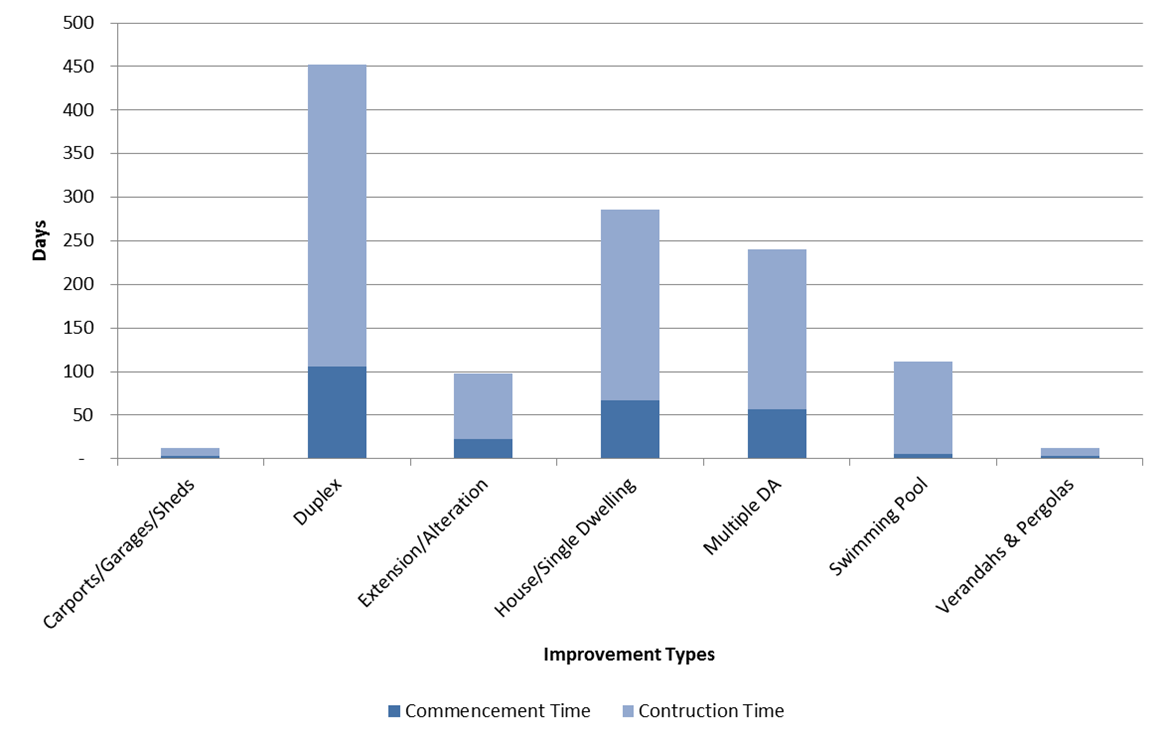
\includegraphics[width=\columnwidth]{Figures/Cm_ct_times.png} \par
 \caption{Average Commencement and Construction times (Days)}
 \label{fig:Cm_ct_times}
\end{figure}


%% Table created by stargazer v.5.2 by Marek Hlavac, Harvard University. E-mail: hlavac at fas.harvard.edu
% Date and time: Wed, Jun 14, 2017 - 04:16:13 AM
% Requires LaTeX packages: dcolumn rotating 
\begin{sidewaystable}[!htbp] \centering
  \caption{Fixed Effect Model Results - DA only sample} 
  \label{results_DA_only_sample} 
    \resizebox{0.9\textwidth}{!}{
\begin{tabular}{@{\extracolsep{5pt}}lD{.}{.}{-3} D{.}{.}{-3} D{.}{.}{-3} D{.}{.}{-3} D{.}{.}{-3} } 
\\[-1.8ex] 
\toprule \\[-1.8ex] 
\\[-1.8ex] & \multicolumn{5}{c}{Log(Resale Price/Purchase Price (Notional))} \\ 
\\[-1.8ex] & \multicolumn{1}{c}{(1)} & \multicolumn{1}{c}{(2)} & \multicolumn{1}{c}{(3)} & \multicolumn{1}{c}{(4)} & \multicolumn{1}{c}{(5)}\\ 
\midrule \\[-1.8ex] 
 Carports/Garages/Sheds & 0.029 & -0.193^{***} & -0.037 & -0.040 & -0.102 \\ 
  & (0.068) & (0.069) & (0.112) & (0.112) & (0.113) \\ 
  & & & & & \\ 
 Duplex & 0.271^{***} & 0.012 & 0.043 & 0.038 & -0.018 \\ 
  & (0.068) & (0.070) & (0.113) & (0.113) & (0.114) \\ 
  & & & & & \\ 
 Extension/Alteration & 0.102 & -0.156^{**} & -0.052 & -0.054 & -0.110 \\ 
  & (0.067) & (0.068) & (0.112) & (0.112) & (0.113) \\ 
  & & & & & \\ 
 House/Single Dwelling & 0.009 & -0.264^{***} & -0.169 & -0.171 & -0.227^{**} \\ 
  & (0.068) & (0.069) & (0.113) & (0.112) & (0.113) \\ 
  & & & & & \\ 
 Multiple DA & 0.122^{*} & -0.149^{**} & -0.058 & -0.061 & -0.121 \\ 
  & (0.068) & (0.069) & (0.113) & (0.112) & (0.113) \\ 
  & & & & & \\ 
 Swimming Pool & 0.257^{***} & 0.001 & -0.023 & -0.024 & -0.087 \\ 
  & (0.068) & (0.069) & (0.112) & (0.112) & (0.113) \\ 
  & & & & & \\ 
 Verandahs/Pergolas & 0.119^{*} & -0.107 & -0.039 & -0.042 & -0.102 \\ 
  & (0.068) & (0.069) & (0.112) & (0.112) & (0.113) \\ 
  & & & & & \\ 
 MktReturn & 0.900^{***} & 0.891^{***} & 0.801^{***} & 0.839^{***} & 0.839^{***} \\ 
  & (0.010) & (0.010) & (0.012) & (0.016) & (0.016) \\ 
  & & & & & \\ 
 Months between sales &  &  &  & -0.000 & -0.000 \\ 
  &  &  &  & (0.000) & (0.000) \\ 
  & & & & & \\ 
 Months between sales squared &  &  &  & -0.000 & -0.000 \\ 
  &  &  &  & (0.000) & (0.000) \\ 
  & & & & & \\ 
 No. of beds (resale) &  & 0.019^{***} & 0.028^{***} & 0.028^{***} &  \\ 
  &  & (0.002) & (0.003) & (0.003) &  \\ 
  & & & & & \\ 
 No. of baths (resale) &  & 0.073^{***} & 0.086^{***} & 0.086^{***} &  \\ 
  &  & (0.003) & (0.003) & (0.003) &  \\ 
  & & & & & \\ 
 No. of cars (resale) &  & 0.013^{***} & 0.011^{***} & 0.011^{***} &  \\ 
  &  & (0.002) & (0.002) & (0.002) &  \\ 
  & & & & & \\ 
 No. of beds (purchase) &  &  & -0.042^{***} & -0.042^{***} &  \\ 
  &  &  & (0.003) & (0.003) &  \\ 
  & & & & & \\ 
 No. of baths (purchase) &  &  & -0.077^{***} & -0.077^{***} &  \\ 
  &  &  & (0.004) & (0.004) &  \\ 
  & & & & & \\ 
 No. of cars (purchase) &  &  & -0.023^{***} & -0.023^{***} &  \\ 
  &  &  & (0.002) & (0.002) &  \\ 
  & & & & & \\ 
 Change in no. of beds &  &  &  &  & 0.034^{***} \\ 
  &  &  &  &  & (0.003) \\ 
  & & & & & \\ 
 Change in no. of baths &  &  &  &  & 0.082^{***} \\ 
  &  &  &  &  & (0.003) \\ 
  & & & & & \\ 
 Change in no. of cars &  &  &  &  & 0.015^{***} \\ 
  &  &  &  &  & (0.002) \\ 
  & & & & & \\ 
Year Fixed Effects & Yes & Yes & Yes & Yes & Yes \\ 
Location Fixed Effects & Yes & Yes & Yes & Yes & Yes \\ 
Observations & \multicolumn{1}{c}{55,732} & \multicolumn{1}{c}{52,735} & \multicolumn{1}{c}{20,366} & \multicolumn{1}{c}{20,366} & \multicolumn{1}{c}{20,366} \\ 
Adjusted R$^{2}$ & \multicolumn{1}{c}{0.481} & \multicolumn{1}{c}{0.497} & \multicolumn{1}{c}{0.494} & \multicolumn{1}{c}{0.494} & \multicolumn{1}{c}{0.493} \\ 
F Statistic & \multicolumn{1}{c}{2,070.625$^{***}$ (df = 25; 55707)} & \multicolumn{1}{c}{1,864.943$^{***}$ (df = 28; 52707)} & \multicolumn{1}{c}{641.274$^{***}$ (df = 31; 20335)} & \multicolumn{1}{c}{603.184$^{***}$ (df = 33; 20333)} & \multicolumn{1}{c}{660.114$^{***}$ (df = 30; 20336)} \\ 
\bottomrule \\[-1.8ex] 
\textit{Notes:} & \multicolumn{5}{l}{Robust standard errors in parentheses. *** 0.1\% significance ** 1\% significance * 5\% significance . 10\% significance} \\ 
\end{tabular}
}
\end{sidewaystable} 
\clearpage


%\section{Appendix C}
\begin{figure}[!htb]
    \centering
     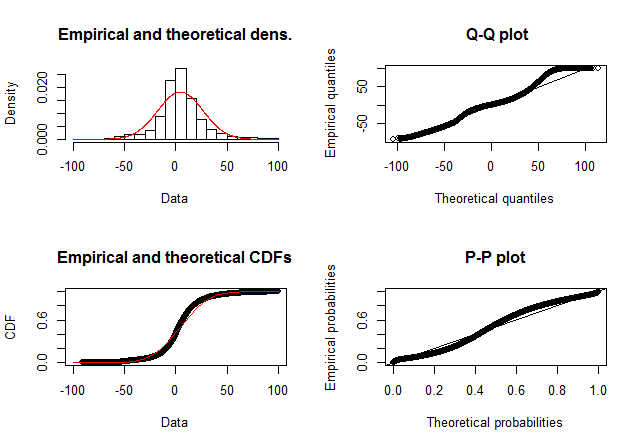
\includegraphics[width=\columnwidth]{Figures/Rplot_qqplot.png} \par
 \caption{House Price Index Prediction Error Distribution}
 \label{fig:Rplot_ssd_err_10}
\end{figure}

\section{}


\end{document}

